\documentclass[titlepage,oneside, 12pt]{book}
\usepackage{url}
\usepackage[toc,page]{appendix}
\usepackage{listings}
\usepackage{tikz}
\usetikzlibrary{calc}
\usetikzlibrary{trees}
\usepackage{amssymb}
\usepackage{float}
\usepackage{amsmath}
\usepackage{amsthm}
\usepackage{ mathrsfs }
\usepackage{tabulary}
\usepackage{booktabs}
\usepackage{mathtools}
\usepackage{caption}
\usepackage{subcaption}
\DeclarePairedDelimiter{\ceil}{\lceil}{\rceil}
\newcommand*{\Comb}[2]{{}^{#1}C_{#2}}%
\usepackage{algorithm}% http://ctan.org/pkg/algorithm
\usepackage{algpseudocode}% http://ctan.org/pkg/algorithmicx
\usepackage{caption}% http://ctan.org/pkg/caption
\usepackage{graphicx}
\graphicspath{ {E:/Users/"Kaeze Phoenix"/Desktop/"Project Masters"/"Referrence Images"/}{E:/Users/"Kaeze Phoenix"/Desktop/"Project Masters"/"Referrence Images"/BP640/ }}


\newtheoremstyle{break}
  {\topsep}{\topsep}%
  {\itshape}{}%
  {\bfseries}{}%
  {\newline}{}%
\theoremstyle{break}
\newtheorem{theorem}{Theorem}


\begin{document}
\sloppy
\title{Compressed Sensing in MRI}
\author{Kashif Hussain \\ ID: 8444507 \\ Supervisor: Oliver Dorn \\ Course Code: MATH4000}
\date{May 10, 2016}
\maketitle

%http://tex.stackexchange.com/questions/119805/bibliography-in-texmaker

\tableofcontents

\chapter*{Preface}
My project is devoted to understanding the role and applications of Compressed Sensing (CS) in Magnetic Resonance Imaging (MRI). The focus is on demonstrating the application of compressed sensing in  MRI through the use of a variety of algorithms. Numerical experiments will be performed with the following algorithms, namely: Basis Pursuit (BP), Orthogonal Matching Pursuit (OMP) and Compressive Sampling Matching Pursuit (CoSaMP). 

Prior knowledge may be useful in the following areas:
\begin{itemize}
\item \textbf{Linear Algebra/Matrix Algebra}:
As I will be using Matlab for my numerical experiments, knowledge of linear algebra and how matrices are defined and treated would be useful in understanding the code in the Appendix. A glance at MATLAB's refresher page would help you understand most of what was written down. 


\item \textbf{Signal Processing Basics}:
Knowledge of Fourier Transforms (FT), Discrete Cosine Transforms (DCT) and Discrete Wavelet Transforms (DWT) would be useful. Having some background in signal processing and understanding what the Nyquist rate is (introduced almost immediately) will help in understanding the topic of compressed sensing quickly. Some of the signals we will use will be sparse in the time domain, however, MRI images are not sparse and need to be transformed for use in compressive sensing techniques. Transformations to sparse domains are at the heart of compressed sensing. 

\item \textbf{Compression Techniques}:
This ties in heavily with signal processing. Whilst knowledge of such techniques is not necessary, they will help in the understanding of the techniques employed in my project. Familiarity with JPEG and its use of the Discrete Cosine Transform which will help point out similarities between my use and that in JPEG.

\end{itemize}

\section*{Chapter Breakdown}

\begin{itemize}
\item \textbf{Chapter 1}: Chapter one introduces the Nyquist-Shannon sampling theorem and how it relates to compressed sensing. In addition, I will introduce the concept of compressed sensing with a brief example as well as an introduction as to how MRI scans work. The chapter ends in detailing the role of compressed sensing in MRI. 

\item \textbf{Chapter 2}: Chapter two is very brief and outlines an important property called the Restricted Isometric Property (RIP) which many algorithms I explore rely on for certain theorems. 

\item \textbf{Chapter 3}: Chapter 3 introduces some of the basic algorithmic approaches to compressed sensing. Some of the algorithms will not be explored in detail and those that are, are given a brief introduction. Model-based compressed sensing, whilst covering a large portion of this chapter, is not experimented with but was discussed in detail due to its expansiveness. 

\item \textbf{Chapter 4}: Chapter 4 covers 3 main algorithms: Basis Pursuit, Orthogonal Matching Pursuit and Compressive Sampling Matching Pursuit. In addition, numerical experiments are carried out on 1-D signals, noise-perturbed signals and finally 2-D MRI images. A breakdown is given on the performance of each of these algorithms with respect to PSNR, running time and the the error produced by the difference in the reconstructed image and original image. 

\item \textbf{Chapter 5}: Chapter 5, the final chapter, marks the end of my project and summarizes the essential information gathered. Using the criterion I developed in chapter 3, I state which algorithms satisfy each criterion.  

\item \textbf{Appendix}: The appendix located at the back of this report details the code use to present the results located within. Some of the code may need to be modified to output certain results. All of the code was written in MATLAB. 

\end{itemize}


\begin{table}[htbp]\caption{Table of Notation}
\begin{center}% used the environment to augment the vertical space
% between the caption and the table
\begin{tabular}{c c p{10cm} }
\toprule
\multicolumn{3}{c}{}\\
\multicolumn{3}{c}{\underline{Fields}}\\
\multicolumn{3}{c}{}\\
$\mathbb{R}$ & $:=$ & Field of real numbers.\\
$\mathbb{C}$ & $:=$ & Field of complex numbers.\\
$\mathbb{F}$ & $:=$ & Any field.\\
\multicolumn{3}{c}{}\\
\multicolumn{3}{c}{\underline{Vector Notation}}\\
\multicolumn{3}{c}{}\\
$\textbf{x} \in \mathbb{F}^{N \times 1}$ & $:=$ &$N\times1$ column vector with N entries from a field $\mathbb{F}$.\\
$x \in \mathbb{F}$ & $:=$ & A scalar quantity in a given field $\mathbb{F}$.\\
$\textbf{x}_{i}$ & $:=$ & The ith entry in the vector \textbf{x}.\\
$\textbf{x}^{(i)}$ & $:=$ & The ith iteration of \textbf{x} in an algorithm.\\
$supp(\textbf{x})$ & $:=$ & The position of the non-zero values of \newline \textbf{x} = \big\{i : $\textbf{x}_i \neq 0$ \big\}. \\
\multicolumn{3}{c}{}\\
\multicolumn{3}{c}{\underline{Matrix Notation}}\\
\multicolumn{3}{c}{}\\
$\textbf{A} \in \mathbb{F}^{M \times N}$ & $:=$ &$M \times N$ matrix with entries from from a field $\mathbb{F}$.\\
$\textbf{A}_{i,j}$ & $:=$ &The (i,j)th entry of \textbf{A}.\\
$\textbf{A}^{T}$ & $:=$ &The transpose of \textbf{A}.\\
$\textbf{A}^{\dagger}$ & $:=$ &The pseudo-inverse of \textbf{A}.\\
\multicolumn{3}{c}{}\\
\multicolumn{3}{c}{\underline{Norm Notation}}\\
\multicolumn{3}{c}{}\\
$|x| $ & $:=$ &The absolute value of the scalar x.\\
$||\textbf{x}||_1 $ & $:=$ &The $\ell_1$-norm: $\sum_{i=1}^{n}|x_i|$.\\
$||\textbf{x}||_2 $ & $:=$ &The $\ell_2$-norm: $\sqrt{\sum_{i=1}^{n}|x_i|^2}$.\\
$||\textbf{x}||_p $ & $:=$ &The $\ell_p$-norm: $\bigg(\sum_{i=1}^{n}|x_i|^{p}\bigg)^{1/p}$.\\
\multicolumn{3}{c}{}\\
\multicolumn{3}{c}{\underline{Other Notation}}\\
\multicolumn{3}{c}{}\\
$\mathbb{P}(A)$ & $:=$ & Probability of event A\\

\bottomrule
\end{tabular}
\end{center}
\label{tab:TableOfNotationForMyResearch}
\end{table}


\chapter{Introduction to Compressed Sensing}

\section{The Nyquist-Shannon Sampling \protect\\ Theorem}

Before introducing what compressed sensing actually is, we must first understand the importance of the Nyquist rate. The sampling theorem relies on a signal whose Fourier transform is zero outside a certain frequency range and this is known as bandlimiting. The Nyquist-Shannon sampling theorem states that perfect reconstruction  of a bandlimited signal requires the sampling rate to be, at minimunum, twice the maximumum frequency found in the bandlimited signal.\cite{NyquistWiki} 

For example, given $x(t)$ is a function of continuous time with a Fourier transform $X(f)$, we find the following equation: 

\begin{equation} 
\begin{gathered}
X(f) = \int_{\infty}^{\infty} x(t) e^{i 2 \pi f t} dt.
\end{gathered}
\end{equation}

In mathematical terms, for the bandlimited signal $x(t)$, we have that the Fourier transform of such a signal obeys the following:

\begin{gather}
\exists B \in \mathbb{R} \quad \textrm{such that} \quad X(f) = 0 \quad \forall |f| > B.
\end{gather}

A sufficient sample-rate is 2B samples/second, or anything larger.

\newpage

 Equivalently, for a given sample rate $f_s$, perfect reconstruction of the signal is guaranteed possible if $f_s > 2B$.  If the bandlimit is too large or is non-existant, aliasing will be introduced after reconstruction and similarly if $f_s$ is less than $2B$. The two thresholds $2B$ and $f_s$ are known as the Nyquist rate and the Nyquist frequency respectively. Figure~\ref{fig:Fex}  shows the Fourier transform of the above signal $x(t)$. 

\begin{figure}[H]
\centering
\includegraphics[scale=0.3]{604px-Bandlimited.png}\caption{The Fourier transform of the bandlimited function $x(t)$ (amplitude against frequency)\cite{NyquistWiki}}
\label{fig:Fex}
\end{figure}

In the medical field and specifically in the MRI field, Nyquist's sampling rate is still too large. The goal is to reduce a patient's exposure to electromagnetic radiation and in order to carry out this goal, we need to take as few samples as possible whilst still reconstructing the scanned image to a high degree of accuracy. This leads to the introduction of compressed sensing which exploits the sparsity of an image to reconstruct the image at a rate far below the Nyquist rate. 

\newpage


%figure~\pageref{fig:fig1}


%https://www.sharelatex.com/learn/Inserting_Images

\section{What is Compressed Sensing}

Throughout the science and technology industry, there are tasks which require you to retrieve data of some importance from a measurable piece of information. We can use compressed sensing to perform such a task.    
Compressed sensing is a signal processing technique which is used to efficiently acquire and reconstruct signals by finding solutions to underdetermined linear systems (i.e. fewer equations than unknowns)\cite{Wikipedia}. The equations in (\ref{eq:UD}) show an underdetermined system of equations with no solutions.  


\begin{equation}
\label{eq:UD}
\begin{split}
a + b + c &= 1,
\\
a + b + c &= 2.
\end{split}
\end{equation}


Compressive sensing exploits the sparsity of a signal/image to recover the signal/image at a rate far below Nyquist rate. As current technology depends heavily on the acquisition and processing of many signals/data (i.e. MRI/CT scans), the process of retrieving compressible signals and reconstructing them can be greatly improved by acquiring them in a compressed form. From this, we can produce an excellent approximation of the actual data through the use of various methods you will see inside this report. Compressible data approximates the data being compressed accurately, but has far fewer non-zero entries. 

When the signal/data acquisition process is linear, the problem is reduced to solving a linear system of equations. As a result, the problem of compressed sensing is to find a $k$-sparse solution to an underdetermined system of linear equations. We refer to a vector as $k$-sparse if, at most, $k$ of its co-ordinates are non-zero. The matrix in figure~\ref{fig:kSparse1} demonstrates a $k$-sparse matrix when $k = 6$

%A_{m,n} = 
% \begin{pmatrix}
%  a_{1,1} & a_{1,2} & \cdots & a_{1,n} \\
%  a_{2,1} & a_{2,2} & \cdots & a_{2,n} \\
%  \vdots  & \vdots  & \ddots & \vdots  \\
%  a_{m,1} & a_{m,2} & \cdots & a_{m,n} 
% \end{pmatrix}


\begin{figure}[H]
\centering
$
\textbf{X}_{4,5} = \begin{pmatrix}
1 & 0 & 0 & 0 & 0 \\
0 & 2 & 0 & 3 & 3 \\
0 & 0 & 0 & 0 & 0 \\
0 & 4 & 0 & 0 & 5 \\
\end{pmatrix}
$
\caption{6-Sparse 4 by 5 Matrix}
\label{fig:kSparse1}
\end{figure}


\newpage

As an example, the process of recovering an image from sampled data is as follows: 

Given $M$ measurements of the measured data, we need to recover the vector (the signal) $\textbf{x}$ from the observed data $\textbf{b}$ whilst letting the matrix $\textbf{A}$ represent the process of reading the signal. So given $\textbf{A} \space \in \mathbb{R}^{M \times N}$,  $\textbf{x} \in \mathbb{R}^{N \times 1}$, $\textbf{b} \in \mathbb{R}^{M \times 1}$ as described as well as $M < N$, such a system is can be written in the form:

\begin{equation}
\begin{gathered}
\textbf{Ax} = \textbf{b}.
\end{gathered}
\end{equation}

Figure~\ref{fig:AxForm} is an illustration of all the ingredients in the compressive sensing process:

\begin{figure}[H]
\centering
$
\textbf{A}_{m, n} = \begin{pmatrix}
  a_{1,1} & a_{1,2} & \cdots & a_{1,n} \\
  a_{2,1} & a_{2,2} & \cdots & a_{2,n} \\
  \vdots  & \vdots  & \ddots & \vdots  \\
  a_{m,1} & a_{m,2} & \cdots & a_{m,n} 
\end{pmatrix}  
$,
$
\textbf{x}_{n, 1} = \begin{pmatrix}
x_{1,1} \\
x_{2,1} \\
\vdots  \\
x_{n,1} 
\end{pmatrix}  
$,
$
\textbf{b}_{m, 1} = \begin{pmatrix}
b_{1,1} \\
b_{2,1} \\
\vdots  \\
b_{m,1} 
\end{pmatrix}  
$.

\caption{The vectors and matrices for $\textbf{Ax}= \textbf{b}$}
\label{fig:AxForm}
\end{figure}


Constructing such a system raises a few questions:
\begin{itemize}
\item Can we reconstruct signal $\textbf{x} \in \mathbb{R}^{N \times 1}$ given {$\textbf{Ax}=\textbf{b}$}? 
\item What matrices $\textbf{A} \in \mathbb{R}^{M \times N}$ are appropriate?
\end{itemize}

Whilst the two questions are closely related, there are in-fact numerous recovery algorithms (discussed later) dedicated to the task of reconstructing the signal $\textbf{x}$. However, the design of the matrix $\textbf{A}$, the measurement matrix, is equally important and through various breakthroughs in the field, results were found to be the best through the use of \textit{random matrices}.

Bernoulli matrices whose entries are +1 or -1 with equal probability and Gaussian matrices formed from a normal distribution are some examples of random matrices. The key point being, that a Gaussian or Bernoulli $M \times N$ matrix $\textbf{A}$, with randomly generated coefficients, can reconstruct any $K$-sparse vectors $\textbf{x}$ from {$\textbf{Ax}=\textbf{b}$} through recovery algorithms. 

\newpage

To summarize, we have the following:
\begin{itemize}
\item $\textbf{x}$ - $N \times 1$ vector which represents our original signal. 
\item $\textbf{b}$ - $M \times 1$ vector which represents our output values.
\item $\textbf{A}$ - $M \times N$ measurement matrix (i.e. getting from input to output) and $M < N$
\end{itemize}

\newpage
 
\section{Simple Compressive Sensing Example}

To illustrate what compressive sensing is about, I will demonstrate by showing a simple example. Let $\textbf{x}$ 
be a $4 \times 9$ vector of random values. We would like to keep only 4 of these values namely the 1st, 4th, 7th and 9th.

\begin{figure}[H]
\centering
$
\textbf{A}_{4,9} = \begin{pmatrix}
1 & 0 & 0 & 0 & 0 & 0 & 0 & 0 & 0 \\
0 & 0 & 0 & 1 & 0 & 0 & 0 & 0 & 0 \\
0 & 0 & 0 & 0 & 0 & 0 & 1 & 0 & 0\\
0 & 0 & 0 & 0 & 0 & 0 & 0 & 0 & 1 \\
\end{pmatrix}  
$
$,
\textbf{x}_{9,1} = \begin{pmatrix}
0.61\\
0.01\\
0.04\\
0.12\\
0.38\\
0.83\\
0.42\\
0.94\\
0.76\\
\end{pmatrix}  
$,
$
\textbf{b}_{4, 1} = \begin{pmatrix}
0.61\\
0.12\\
0.42\\
0.76\\
\end{pmatrix}  
$.

\caption{A simple example of $\textbf{Ax} = \textbf{b}$}
\label{fig:CSex1}
\end{figure}

In figure~\ref{fig:CSex1}, we keep only 4 samples of our original data and discard the remaining 5. However, in the context of medical imaging, our original data \textbf{$x$} is usually sparse under specific transforms and as such our measurement matrix \textbf{$A$} is inappropriate. This is because we do not know the location of the most important and useful values of the original data beforehand and as such, we may end up discarding them with our present measurement matrix. So now, suppose \textbf{x} is sparse as below. 

\begin{figure}[H]
\centering
$
\textbf{A}_{4,9} = \begin{pmatrix}
1 & 0 & 0 & 0 & 0 & 0 & 0 & 0 & 0 \\
0 & 0 & 0 & 1 & 0 & 0 & 0 & 0 & 0 \\
0 & 0 & 0 & 0 & 0 & 0 & 1 & 0 & 0\\
0 & 0 & 0 & 0 & 0 & 0 & 0 & 0 & 1 \\
\end{pmatrix}  
$,
$
\textbf{x}_{9,1}\begin{pmatrix}
0.61\\
0.01\\
0.04\\
0\\
0\\
0\\
0.42\\
0\\
0\\
\end{pmatrix}  
$,
$
\textbf{b}_{4, 1} = \begin{pmatrix}
0.61\\
0\\
0.42\\
0\\
\end{pmatrix}  
$.

\caption{Showing the effect of an inappropriate choice for $\textbf{A}$ on our output values $\textbf{b}$ - we lose essential information}
\label{fig:CSex2}
\end{figure}

\newpage
We require a new approach towards creating our measurement matrix $\textbf{A}$. As discussed before, we can use \textit{random matrices} for an effective measurement matrix and then use recovery algorithms on our output values $\textbf{b}$ to get a close approximation for our original data $\textbf{x}$. As an example, we can use a Gaussian matrix as in figure \ref{fig:CSex3}. Our output is different from the original $\textbf{x}$, but the original values are still encoded into the entries of $\textbf{b}$. 

\begin{figure}[H]
\centering
$
\textbf{A}_{4,9} = \begin{pmatrix}
0.09  	&0.73	&0.61	&-0.25	&1.26	&0.55	&-0.26	&0.22	&-1.22\\
-1.50	&-0.60	&-0.01 	&0.80	&0.16 	&-0.02	&0.37 	&-0.91	&-0.03\\
0.21	&-0.43	&0.10	&1.15	&1.78	&-1.99	&-0.86	&-2.59	&1.43\\
-0.99	&-0.37	&-2.24	&0.26	&0.73	&-1.07	&-0.94 	&0.18	&-0.41
\end{pmatrix}  
$,
$
\textbf{x}_{9,1}\begin{pmatrix}
0.61\\
0.01\\
0.04\\
0\\
0\\
0\\
0.42\\
0\\
0\\
\end{pmatrix}  
$,
$
\textbf{b}_{4, 1} = \begin{pmatrix}
-0.02\\
-0.77\\
-0.23\\
-1.09\\
\end{pmatrix}  
$.

\caption{Obtaining 4 output values using Gaussian random variables for our measurement matrix $\textbf{A}$}
\label{fig:CSex3}
\end{figure}

Figure~\ref{fig:CSex3} shows a system with some knowns, unknowns and, in particular, one assumption. With this information at our disposable, we need to recover our original vector $\textbf{x}$. It is at this point that we make use of compressed sensing recovery algorithms to retain a close approximation to the original vector $\textbf{x}$. 

\newpage

\begin{flushleft}
A summary of the information attained from figure~\ref{fig:CSex3}:
\end{flushleft}

Known:

\begin{itemize}
\item The $4 \times 9$ measurement matrix $\textbf{A}$ which was randomly generated with Gaussian random variables.
\item The $ 4 \times 1$ output vector $\textbf{b}$.
\end{itemize}

Unknown: 
\begin{itemize}
\item The $ 9 \times 1$ original vector $\textbf{x}$.
\end{itemize}

The Assumption: 
\begin{itemize}
\item The $ 9 \times 1$ original vector $\textbf{x}$ is sparse.
\end{itemize}

\begin{flushleft}
To summarize:
\end{flushleft}
In the context of compressively sensing MRI images, we need the measurement matrix to be able to encode the values present in the sparse domain of the image into the output vector so that no value is discarded. Following the encoding of the transform data, we make use of a recovery algorithm to approximate the values of the original sparse domain of the image from our encoded data. 

The following section details what Magnetic Resonance Imaging (MRI) scans are and how the a scan is achieved as well as the importance and applications of compressed sensing in MRI 

\newpage

\section{How MRI Scans work}
Most of the human body is comprised of water (about 70\%) and each water molecule is comprised of hydrogen and oxygen atoms. Hydrogen atoms have a strong magnetic moment, which means that in a magnetic field, the protons in the centre of these hydrogen atoms which are sensitive to magnetic fields and have a positive charge, line up in the direction of the field. 
 
Laying down under an MRI scanner magnetizes the protons so that half point to the patient's feet and the other half point to the patient's head. As a result, most of the protons cancel each other out meaning that for each proton facing the patient's head, there is a proton facing the patient's feet so that they differ by approximately 180 degrees. However, as there millions of protons inside the human body, some are not canceled out.  Following the alignment of the protons, short bursts of radio waves, specific to hydrogen atoms, are sent to designated areas of the body. These radio frequency pulses (RF) distort the alignment of those unmatched protons which absorb the energy and these protons begin to spin at a particular frequency and direction. When the burst of radio frequency pulses stop, the protons realign so that they face their original direction inside the magnetic field whilst releasing the energy absorbed from the RF pulses by sending out their own radio signals which are picked up by receivers.\cite{NHS-MRI}


From this, the system now knows the location of the protons inside your body. Like the amalgamation of sound produced by the notes of a piano all point to certain signals, MRI scanners detects tissues like a musician would detect the intensity or type of note. This is because the various types of tissues in your body have protons which align at different speeds and so they all send their own distinct and identifiable signals.

Whilst, on its own, a single proton may not provide useful information, using these millions of signals from the protons in the body, you can reconstruct a a high-resolution image of the internal body like pixels on a computer screen. Figure~\ref{fig:MRIScan} provides a visual illustration of how MRI scans work.  
 
\begin{figure}[t!]
\centering
\centerline{\includegraphics[scale=0.9]{mri-steps.jpg}}
\caption{How an image is formed from an MRI scan\cite{HSW-MRI}}
\label{fig:MRIScan}
\end{figure}


\clearpage

%Edit this chapter perhaps
\section{Compressed Sensing in MRI}
Image compression is an area of research which has been thoroughly studied. Take for example well-known image compression tools such as JPEG which makes use of the Discrete Cosine Transform (DCT). This transform is useful in its ability to transform the image content into a vector of sparse coefficients. The widespread success and use of image compression algorithms such as JPEG makes us question whether or not we need to acquire all the data in the first place as the data is clearly compressible. Why not just retrieve the compressed information directly? As a result, in order to reduce patient's exposure to electromagnetic radiation and reduce scan times, compressive sensing is heavily studied in the medical imaging field.

Magnetic Resonance Imaging (MRI) is a common technology in medical imaging. It is used for various tasks such as brain imaging, heart imaging, examining blood vessels and more. The time taken to produce high-resolution images can range between several minutes up to hours depending on the task. In emergency situations, the usefulness of compressive sensing is highlighted by its ability to speed up the imaging process. As a result, speeding up the scanning time has always been of interest to those researching medical imaging. In recent years, compressed sensing has been touted to be able to achieve accurate reconstruction of signals which are sparse or can be compressed from undersampled measurements (such as MRI/CT scans). As a result, through the use of compressive sensing in MRI, we can cut-down scanning time of MRI scans and produce accurate image reconstruction with the only assumptions about the MRI image used is that it is compressible or sparse in a transform domain. 

High quality reference images with similar structure to that of the target image can be acquired easily in various practical MRI applications. Using such a reference image to get prior information can further decrease the number of measurements we need to take. The problems which needs to be overcome by compressive sensing in MRI is that when the $K$-space is undersampled, the Nyquist criterion is violated and reconstructions show artefacts. The 2D or 3D Fourier transform of an MRI image is known as the $K$-space and it is utilized as, in general, MRI images are not sparse and they require to be transformed into a sparse domain to apply compressive sensing techniques. Figure~\ref{fig:3d} shows a three-level wavelet decomposition. 

An image is represented by a two-dimension array of coefficients where each coefficient corresponds to the colour or brightness of that point. Using the fact that most natural images have smooth colour variations with details being sharper at edges, we can treat the smooth variations of colour as low frequency variations and the sharp as high frequency.

Both frequencies play an important role and can be described as follows:

\begin{itemize}
\item \textbf{Low Frequency}: This makes up the base of the image.
\item \textbf{High Frequency}: This frequency improves upon the base provided by the low frequency and refines the image resulting in a more detailed image. 
\end{itemize}

We can separate the low frequencies of an image from the high by using a wavelet transform and the one I will be using in my experiments on MRI images will be the Direct Wavelet Transform (DWT). We can order the bands in the image by importance with $LL_3$ being the most important and the order decreases as you move to a higher decomposition level. From these coefficients, we are able to inverse the transform and retain our original image.


\begin{figure}[h]
\begin{center}

\begin{tikzpicture}
\draw (0,0) -- (8,0) -- (8,8) -- (0,8) -- (0,0);
\draw (0,4) -- (4,4) -- (4,0);
\draw (8,4) -- (4,4);
\draw (4,8) -- (4,4);
\draw (2,4) -- (2,6);
\draw (4,6) -- (2,6);
\draw (2,8) -- (2,6);
\draw (0,6) -- (2,6);
\draw (0,7) -- (1,7);
\draw (2,7) -- (1,7);
\draw (1,6) -- (1,7);
\draw (1,8) -- (1,7);
\node (LL_3) at (0.5, 7.5) {\tiny $LL_{3}$};
\node (HL_3) at (1.5, 7.5) {\tiny $HL_{3}$};
\node (LH_3) at (0.5, 6.5) {\tiny $LH_{3}$};
\node (HH_3) at (1.5, 6.5) {\tiny $LL_{3}$};
\node (HL_2) at (3, 7) {$HL_{2}$};
\node (HH_2) at (3, 5) {$HH_{2}$};
\node (LH_2) at (1, 5) {$LH_{2}$};
\node (HL_1) at (6, 6) {\LARGE $HL_{1}$};
\node (HH_1) at (6, 2) {\LARGE $HH_{1}$};
\node (LH_1) at (2, 2) {\LARGE $LH_{1}$};
\end{tikzpicture}
\caption{A 3 level decomposition  of a "Discrete Wavelet Transform" (DWT) }
\label{fig:3d}
\end{center}
\end{figure}



\newpage
As mentioned earlier, undersampling the $K$-space will results in artefacts. There are many ways to mitigate artefacts as a result of undersampling: 
\begin{itemize}
\item[1] Use methods in which artefacts are less visually apparent to the viewer. 
\item[2] Exploit the $K$-space redundancy by using parallel imaging or other techniques
\item[3] Exploit the spatial/temporal redundancy or both\cite{sparseMRI}.
\end{itemize}

To get an idea of compressive sensing in MRI, we can represent its undersampling process mathematically. We can form the sampling matrix and its Fourier transform as follows:
\begin{itemize}
\item $\textbf{S} \in \mathbb{C}^{M \times N}$ represent the sampling matrix with $m < n $,

\item $\textbf{F} \in \mathbb{C}^{N \times N}$ is the Fourier transform.
\end{itemize}
Further, as each image has some noise associated with it, let:
\begin{itemize}
\item $\pmb{\eta} \in \mathbb{C}^{M \times 1}$ represent the noise,

\item $\textbf{b} \in \mathbb{C}^{M \times 1}$ being the undersampled $k$-sparse data. 
\end{itemize}
The the original signal is represented as:

\begin{itemize}
\item $\textbf{x} \in \mathbb{C}^{N \times 1}$ the vector produced via MRI. 
\end{itemize}
As a result, we get the following equation: 

\begin{equation}
\begin{gathered}
\pmb{SF}\textbf{x} + \pmb{\eta} = \textbf{b}.
\end{gathered}
\end{equation}

The purpose of image reconstruction then becomes our ability to recover   $\textbf{x} \in \mathbb{C}^{N \times 1}$  produced by Magnetic Resonance Imaging (MRI) from our undersampled data $\textbf{b}$\cite{MRImodel}. Given an idea of how MRI scans work, we must introduce an important property for which many compressed sensing algorithms rely on. 

\newpage

\chapter{Restricted Isometric Property}

In order to transform an $N \times 1$, K-sparse signal vector \textbf{x} to our $ M \times 1 $ output sample vector \textbf{b} we must use some  $ M \times N$ measurement matrix \textbf{A}. This measurement matrix must be able to map two different signals $ \textbf{x}_{1} $ and $ \textbf{x}_{2} $ to two different output signals $ \textbf{b}_{1} = \textbf{Ax}_{1} $ and $ \textbf{b}_{2} = \textbf{Ax}_{2} $.  

In order for this to occur, a certain condition must be satisfied known as the Restricted Isometric Property (RIP) as proposed by Candes and Tao\cite{ICS}:

\newtheorem*{RIP}{Definition RIP}
\begin{RIP}
For each integer K = 1, 2, ..., the isometry constant $\delta_{K}$ of the measurement matrix $\textbf{A}$ is the smallest number such that:

\begin{equation}
\begin{gathered}
(1 - \delta_{K})||\textbf{x}||_{2}^2 \leq ||\textbf{Ax}||_{2}^{2} \leq (1 + \delta_{K})||\textbf{x}||_{2}^{2}
\end{gathered}
\label{eqn:RIP}
\end{equation}
holds for all K-sparse vectors $\textbf{x}$.
\end{RIP}

In addition if $\delta_{K} << 1$ then our measurement matrix \textbf{A} has a large probability of stably reconstructing the $\dfrac{K}{2}$-sparse signal. Whilst $\delta_{K} \geq 1$ is not explicitly forbidden, the relevant use involves $\delta_{K} < 1$. 
Whilst $\delta_{K} < 1$, the inequalities presented in \eqref{eqn:RIP} hold and further implies that all subsets of the K columns from A are almost orthogonal (however, they cannot be exactly orthogonal as we have more columns than rows as $M < N$). 
\newpage
The link between RIP and Compressed Sensing is described as follows: 



\begin{itemize}
\item We want to recover a K-sparse signal using the measurement matrix $\textbf{A}$. 
\item Let $\delta_{2K}$ be sufficiently less than 1.
\end{itemize}


Then all pairwise distances between K-sparse signals must be well persevered in the measurement space which implies: 

\begin{equation}
\begin{gathered}
(1 - \delta_{2K})||\textbf{x}_{1} - \textbf{x}_{2}||_{2}^2 \leq ||\textbf{Ax}_{1} - \textbf{Ax}_{2}||_{2}^{2} \leq (1 + \delta_{2K})||\textbf{x}_{1} - \textbf{x}_{2}||_{2}^{2}
\end{gathered}
\label{eqn:RIP2}
\end{equation}

holds for all K-sparse signal vectors $ \textbf{x}_{1} $ and $ \textbf{x}_{2} $. Further as $ \textbf{x}_{1} $ and $ \textbf{x}_{2} $ are different signal vectors, the following is true: 

\begin{equation}
\begin{gathered}
||\textbf{x}_{1} - \textbf{x}_{2}||_{2}^2 > 0,
\end{gathered}
\label{eqn:fact1}
\end{equation}

\begin{equation}
\begin{gathered}
||\textbf{Ax}_{1} - \textbf{Ax}_{2}||_{2}^2 > 0,
\end{gathered}
\label{eqn:fact2}
\end{equation}

which means that the measurement matrix \textbf{A} maps the two signal vectors to two different output signal vectors $\textbf{b}_{1}$ and  $\textbf{b}_{2}$.
In order to reconstruct a K-sparse signal \textbf{x} from a sample output signal \textbf{b} by means of a stable process, we require the restricted isometry constant $\delta_{2K}$ to be small. Whilst it is computationally difficult to check if a matrix satisfies~\ref{eqn:RIP}, it has been shown that many matrices satisfy the restricted isometry condition with large probability and few measurements. A concrete example would be random Gaussian or Bernoulli matrices which can be shown to satisfy the restricted isometry condition with very high probability. Further, any subguassian measurement matrix can be shown to follow the isometry condition. We define a subgaussian matrix as follows:

\newtheorem*{SG}{Definition Subgaussian}
\begin{SG}
An random variable X is subgaussian if:

\begin{equation}
\begin{gathered}
\mathbb{P}(|X| > t) \leq Ce^{vt^{2}}
\end{gathered}
\label{eqn:SG}
\end{equation}
for all $t > 0$ and some positive constants C and v.  
\end{SG}

The proof of subguassian matrices satisfying the restricted isometry condition is not shown here but can be researched elsewhere. \cite{CST&A}

Following this, we see that any subguassian random matrices have fat-tail distributions which is due to Gaussian random variables. Bernoulli matrices (whose entries are either +1 or -1) are subgaussian which is defined with~\ref{eqn:SG} by choosing $C = \dfrac{1}{e}$ and $v = 1$. Further, we have that the Gaussian matrices (whose entries are identically distributed random variables from a Gaussian probability density function) are subgaussian by choosing $C = v = 1$.

An $M \times N$ subguassian matrix has restricted isometry behavior with large probability if the following condition holds:


\begin{equation}
\begin{gathered}
M > C \cdot K \cdot log(N/K)
\end{gathered}
\label{eqn:fact3}
\end{equation}


where is C some constant depending on the circumstance \cite{CSDon}\cite{RBUC}. Therefore, we can recover K-sparse signals \textbf{x} of length N from output signals \textbf{b} of length M $(M < N)$ after taking  M random Gaussian or Bernoulli measurements through a measurement matrix \textbf{A}. 

Throughout, I will be using a Gaussian random matrix without checking if the above conditions are satisfied as they have been proven to satisfy the restricted isometry condition given they are subgaussian. 

\newpage



\chapter{Introduction to Basic Algorithms}
\section{Introduction}

This section will give a short and succinct introduction to some of the basic algorithms used in compressive sensing with a more detailed look at some of them in chapter 4. Model-based compressed sensing will be discussed in more detail due to its nature. 

Let $||\textbf{x}||_0$ represent the number of non-zero elements in some vector $\textbf{x}$. We want to retrieve the original vector $\textbf{x}$ from the output vector \textbf{b} after sampling it with our measurement matrix \textbf{A}. Mathematically speaking, we want to:

\begin{equation}
\begin{gathered}
\underset{\textbf{x} \in \mathbb{R}^{N \times 1}}{\min ||\textbf{x}||_{0}} \quad
\text{subject to} \quad \textbf{b = Ax}.
\end{gathered}
\end{equation}

We try and locate the sparsest vector possible from the measurable data we have available $\textbf{Ax} = \textbf{b}$. However, $\ell_0$-minimization is non-deterministic polynomial-time hard (NP-hard) and so not very applicable in MRI. This is due to how computationally intensive it is to solve given the fact we want to retrieve MRI scans faster than previously achieved. There is another algorithm called Basis Pursuit or otherwise known as, $\ell_{1}$-minimization which was proven equivalent\cite{delin} to the $\ell_{0}$-minimization problem and is explored in detail in chapter 4. 

\section{Optimization Methods}

\subsection{Basis Pursuit}
Whilst $\ell_0$-minimization is NP-hard and a non-convex optimization problem and therefore potentially very difficult to solve, there exists another algorithm known as $\ell_1$-minimization or Basis Pursuit.

Like $\ell_0$-minimization, Basis Pursuit requires us to:
\begin{equation}
\begin{gathered}
\underset{\textbf{x} \in \mathbb{R}^{N \times 1}}{\min ||\textbf{x}||_{1}} \quad \space \text{subject to} \quad \textbf{b = Ax}.
\end{gathered}
\end{equation}

Basis Pursuit is a convex optimization problem which is easier to solve than a non-convex as there exist accurate solvers. However, it does not take into account the complexity of the problem. An extension to this algorithm provides a solution to a more general case such as the presence of some random noise $\pmb{\eta}$ discussed briefly below, but is explored in chapter 4. 


\subsection{Quadratically Constrained Basis Pursuit}
This algorithm provides a solution to the general case when there is some error in the image and is also known as the noise-aware $\ell_1$-minimization. 

The mathematical representation of the problem is represented as follows: 

\begin{equation}
\begin{gathered}
\underset{\textbf{x} \in \mathbb{R}^{N \times 1}}{\min ||\textbf{x}||_{1}} \quad \space \text{subject to} \quad ||\textbf{Ax - b}||_{2} \le E.
\end{gathered}
\end{equation}

This extension of the original algorithm applies better to the general case as it is very likely that the output signal vector $\textbf{b} \in \mathbb{R}^{M \times 1}$ is not equivalent to the the vector $\textbf{Ax} \in \mathbb{R}^{M \times 1}$ but is of the form $\textbf{Ax} + \pmb{\eta}$ instead where $\pmb{\eta} \in \mathbb{R}^{M \times 1}$ is some error which produces the noise in the output signal.

Given some $E \ge 0$ we can estimate the error produced from our measurements using the $\ell_2$-norm i.e. $||\pmb{\eta}||_2 \le E$. This again is a convex problem and can be solved in numerous ways. The solution to the quadratically constrained algorithm also provides a link to the Basis Pursuit Denoising algorithm which involves solving from some parameter $\lambda \ge 0$ such that we must:\cite{BookMICS}

\begin{equation}
\begin{gathered}
\underset{\textbf{x} \in \mathbb{R}^{N \times 1}}{\min \lambda||\textbf{x}||_{1}} + ||\textbf{Ax - b}||_{2}^{2} \le E.
\end{gathered}
\end{equation}


\newpage

\subsection{Least Squares Solution}
An  $\ell_{2}$-minimization problem, also known as the least squares solution, can also be constructed via the following equation:

\begin{equation}
\begin{gathered}
\underset{\textbf{z }\in \mathbb{R}^{N \times 1}}{\min ||\textbf{z}||_{2}} \quad \text{subject to} \quad \textbf{b} = \textbf{Az},
\end{gathered}
\label{eqn:l2-1}
\end{equation}

where given the transpose of \textbf{A}, which is $\textbf{A}^{T}$, we can use the following to formulate \textbf{z}:

\begin{equation}
\begin{gathered}
||\textbf{z}||_{2} = \textbf{A}^{T}(\textbf{A}\textbf{A}^{T})^{-1}\textbf{b} 
\end{gathered}
\label{eqn:l2-2}
\end{equation}

as the best guess for \textbf{x} in the system \textbf{Ax = b}. 
However, recovering \textbf{x} exactly only occurs under special circumstances. 


\begin{figure}[H]
\centering
\begin{tikzpicture}

\draw[thick,->] (0,0) -- (4.5,0);
\draw[thick,->] (0,0) -- (0,4.5);
\draw[thick,->] (0,0) -- (-4.5,0);
\draw[thick,->] (0,0) -- (0,-4.5);
\def\radius{1cm}
\coordinate (centre) at (0,0);
\draw (centre) circle[radius=\radius];

\path (centre) ++(0.25*180:\radius) coordinate (A);

\fill[black] (A) circle[radius=4pt] ++(0.25*180:1em) node {$\textbf{z}$};

\draw (A) -- ($(A)!4!-90:(centre)$);
\draw (A) -- ($(A)!4!90:(centre)$) node[below]{$\textbf{Ax = b}$};



%\foreach \x in {0,1,2,3,4}
%    \draw (\x cm,1pt) -- (\x cm,-1pt) node[anchor=north] {$\x$};
%\foreach \y in {0,1,2,3,4}
%    \draw (1pt,\y cm) -- (-1pt,\y cm) node[anchor=east] {$\y$};
%\foreach \x in {0,-1,-2,-3,-4}
%    \draw (\x cm,1pt) -- (\x cm,-1pt) node[anchor=south] {$\x$};
%\foreach \y in {0,-1,-2,-3,-4}
%    \draw (1pt,\y cm) -- (-1pt,\y cm) node[anchor=west] {$\y$};

\end{tikzpicture}
\caption{An example of a least squares guess}
\label{fig:L2Tikz}
\end{figure}

Suppose $\textbf{Ax = b}$ then if \textbf{x} is in the Range($\textbf{A}^{T}$) (i.e. in the column space of the measurement matrix \textbf{A}), we can recover \textbf{x} exactly. 

As a result, if $\textbf{x} = \textbf{A}^{T}\textbf{z}$ for some vector 
$\textbf{z} \in \mathbb{R}^{M \times 1}$, then:

\begin{align}
\textbf{A}^{T}(\textbf{A}\textbf{A}^{T})^{-1}\textbf{z} &= \textbf{A}^{T}(\textbf{A}\textbf{A}^{T})^{-1}\textbf{A}\textbf{x}
\\
&=\textbf{A}^{T}(\textbf{A}\textbf{A}^{T})^{-1}\textbf{A}^{T}\textbf{z}
\\
&=\textbf{A}^{T}\textbf{z}
\\
&= \textbf{x}. 
\end{align}
\label{eqn:l2proof}

To conclude, if \textbf{x} lies in some M-dimensional subspace of $\mathbb{R}^{N \times 1}$, it can be recovered from observations through the $M \times N$ measurement matrix \textbf{A}. However, in many cases, the results produced by the least squares solution is not satisfactory and almost never gives a K-sparse solution and as such, I will not be investigating an $\ell_{2}$-minimization. A low level illustration of a least squares solution is shown in figure~\ref{fig:L2Tikz}




\section{Greedy Methods}
Whilst convex optimization methods are some of the most powerful methods for obtaining sparse representations of matrices, there are some iterative or greedy methods for solving similar problems.

Through the use of iterative approximations of the signal coefficients and support, greedy algorithms repetitively identify the support of a signal until some criteria for the convergence is met or it obtains a better approximation of the sparse signal at each iteration accounting for data which doesn't match. 
\newpage
\subsection{Orthogonal Matching Pursuit}\label{OMP}
Orthogonal Matching Pursuit (OMP) is a greedy algorithm I will be investigating in more detail in chapter 4. A thorough analysis on the algorithm is available in a paper by Gilbert and Tropp\cite{GP}. 

Through the use of subgaussian measurement matrices, OMP is able to reconstruct sparse signals. Given a K-sparse signal $\textbf{x} \in \mathbb{R}^{N \times 1}$ and a subguassian matrix $\textbf{A} \in \mathbb{R}^{M \times N}$, the signal \textbf{x} can be represented by a signal \textbf{b = Ax}. Denoting the columns of \textbf{A} as $\textbf{A}_1$, $\textbf{A}_2$, $\textbf{A}_3$, $\ldots$, $\textbf{A}_N$, \textbf{b} can be thought of as a linear combination of the columns of \textbf{A} as \textbf{x} has only K non-zero coefficients. OMP works by greedily picking columns of \textbf{A} to find which participate in the construction of the output signal \textbf{b}. This is done by iteratively locating the largest correlation between the residual of \textbf{b} and \textbf{A}. At each iteration, one coefficient of the support vector is calculated and as a result, we could stop after K iterations for a K-sparse solution. The stopping criteria, however, could be defined as one or more of the following:

\begin{itemize}
\item \textbf{Residue norm:} If the norm of the residue is less than some $E \geq 0$ then we should stop. 
\item \textbf{Reaching target sparsity:} Given the sparsity value K, stop after K iterations. 
\item \textbf{Max number of iterations:} Stop OMP algorithm if iteration count reaches a certain number. 
\end{itemize} 

\newpage
\subsection{Stagewise Orthogonal Matching Pursuit}
Stagewise Orthogonal Matching (StOMP) was introduced by Donoho and his collaborators\cite{STOMP}. StOMP, similarly to OMP, utilizes the signal $\textbf{x} = \textbf{A}^{T}\textbf{b}$ where \textbf{b} = \textbf{Ax} is the usual output signal. It improves on OMP and allows multiple coefficients to be added to the support in one iteration as opposed to OMP only allowing one coefficient to be added per iteration. This is possible due to the introduction of thresholding which allows all coefficients above a certain threshold to be added to the support. Following this, the least-squares problem is solved and updates the residual before iterating.  

In order to describe thresholding strategies below, we need the following definitions:

\newtheorem*{FA}{Definition: False Alarm}
\begin{FA}
A false alarm is the presence of a coefficient in the estimate of the support $\textbf{I}^{(K)} $ but not in the actual support \textbf{I} of the original signal \textbf{x}. 
\end{FA}

\newtheorem*{FD}{Definition: False Discovery}
\begin{FD}
Given that the coefficients in our estimation of the support $\textbf{I}^{(K)}$ are called discoveries, false discoveries are all the coefficients in $\textbf{I}^{(K)}$ but not in the actual support \textbf{I} of the original signal  \textbf{x}, 
\end{FD}



Choosing the thresholding parameter involves choosing between two main strategies:



\begin{itemize}
\item[1] \textbf{False Alarm Control}: The threshold governed by this strategy focuses on limiting the false alarm rate so that it does not exceed a specific number per iteration.

\item[2] \textbf{False Discovery Control}: This threshold is chosen to limit the fraction of incorrectly selected  coefficients in our estimation for the support. 

\end{itemize} 

\newpage

The algorithm for StOMP is defined as follows:

\begin{algorithm}
  \caption{StOMP Algorithm}
  \bigskip	
  \textbf{Inputs}% Inputs section
  \begin{algorithmic}[1]
    \State Measurement matrix $\textbf{A} \in \mathbb{R}^{M \times N}$
    \State Output signal vector $\textbf{b} \in \mathbb{R}^{M \times 1}$
    \State Threshold value: TV
    \State The number of iterations (K) to perform (K = Sparsity value)
  \end{algorithmic}
  \bigskip  
  \textbf{Outputs}%
  \begin{algorithmic}[1]
    \State A K-sparse Signal $\textbf{x}\in \mathbb{R}^{N \times 1}$ which satisfies $\textbf{b} = \textbf{A}\textbf{x}$
  \end{algorithmic}
  \bigskip
  \textbf{Steps}% Steps section
  \begin{algorithmic}[1]
   \Procedure{StOMP}{$A,b,TV,K$}
\State $\textbf{z}^{(0)} \gets 0$
   \State $\textbf{I}^{(0)} \gets \emptyset$
   \For{$i = 1,\ldots,K$}
    %\While{$r\not=0$}\Comment{We have the answer if r is 0}
   \State $\textbf{r}^{(i)} \gets \textbf{b} - \textbf{A}\textbf{z}^{(i-1)}$ \Comment{Get the Residual}
   \State $\textbf{v}^{(i)} \gets \textbf{A}^{T}\textbf{r}^{(i)}$  \Comment{The observation vector}
   \State $\textbf{C}^{(i)} \gets \{j : |v^{(i)}_j| > TV\}$ \Comment{Select coefficients using threshold}
   \State $\textbf{I}^{(i)} \gets \textbf{I}^{(i-1)} \cup \textbf{C}^{(i)}$
   \State $\textbf{z}^{(i)} \gets \textbf{A}^{\dagger}_{\textbf{I}^{(i)}}\textbf{b}$ \Comment{Estimation (Note $\textbf{A}^{\dagger}$ = $(\textbf{A}_{T}\textbf{A})^{-1}\textbf{A}_{T}\textbf{b}$)}
   \EndFor
   
   \State $\textbf{return} \quad \textbf{x} \gets \textbf{z}^{(K)}$
   \EndProcedure

  \end{algorithmic}
  
  %\begin{algorithmic}[1]
  %\textbf{Inputs}% Inputs section
  %  \State Measurement matrix $\textbf{A} \in \mathbb{R}^{M \times N}$
  %  \State Output signal vector $\textbf{b} \in \mathbb{R}^{M \times 1}$
  %  \State Threshold value: TV
  %  \State K number of iterations to perform
  %  \end{algorithmic}
  %   \bigskip	   
  %  \textbf{Outputs}% Inputs section
   % \State \textbf{Initialization} ‎$R^{(0)} = x$
   % \While{$i \leq k$}
    %  \State $l = \displaystyle \argmax_{l = 1,\dots,l} |\langle g_l,R^{(i)} \rangle|$
     %   \comment{finding the atom in dictionary $\mathcal{G}$ ‎with maximum correlation with residual.}
     % \State $R^{(i+1)} = R{(i)}-a_l g_l^{(i)}‎$
     % \State $\hat{x} = \hat{x}+\langle R^{(i)}, g_{l}^{(i)} \rangle g_{l}^{(i)}‎$
      %\State $i = i + 1$
    %\Endwhile
 % \end{algorithmic}
\end{algorithm}

%\begin{algorithm}
%  \caption{StOMP Algorithm}
%  \begin{algorithmic}[1]
%    \REQUIRE Decomposition of signal $x$
%    \INPUT signal $x \in \mathcal{R}^{m}$, Dictionary $\mathcal{G} \in \mathcal{R}^{m \times n‎‎}$, $\hat{x} = \emptyset$
%    \OUTPUT Decomposed signal $\hat{x}_{\text{est}}$ after $k$ iteration, Residual $R^{(k)}$
%    \STATE \textbf{Initialization} ‎$R^{(0)} = x$
%    \WHILE{$i \leq k$}
%      \STATE $l = \displaystyle \argmax_{l = 1,\dots,l} |\langle g_l,R^{(i)} \rangle|$
%        \COMMENT{finding the atom in dictionary $\mathcal{G}$ ‎with maximum correlation with residual.}
%      \STATE $R^{(i+1)} = R{(i)}-a_l g_l^{(i)}‎$
%      \STATE $\hat{x} = \hat{x}+\langle R^{(i)}, g_{l}^{(i)} \rangle g_{l}^{(i)}‎$
%      \STATE $i = i + 1$
%    \ENDWHILE
%  \end{algorithmic}
%\end{algorithm}

I will not be exploring this algorithm due to its similarity with OMP and CoSaMP both of which I will be investigating. 



\newpage

\subsection{Compressive Sampling Matching Pursuit}\label{COSAMP}

Compressive Sampling Matching Pursuit (CoSaMP) is an extension to OMP developed by Needell and Tropp\cite{CoSaMP}. CoSaMP is similar to another algorithm introduce by the same authors known as Regularized Orthogonal Matching Pursuit (ROMP)\cite{ROMP1}. Whilst ROMP is not discussed here, it suffices to note that CoSaMP was constructed to overcome the shortcomings of ROMP. A key difference between the two is that ROMP was designed to select more than one coefficient to be in the support set, which meant ROMP was able to make mistakes in the support set, but was still able to accurately reconstruct the original signal. Further, the uniform guarantees provided by the ROMP algorithms are persevered by CoSaMP without introducing a logarithmic term to the restricted isometric property. 

The goal of CoSaMP is to identify the K largest coefficients in the source signal \textbf{x}. Given that the measurement matrix \textbf{A} satisfies the restricted  isometric property discussed earlier and given that the output signal is \textbf{b = Ax}, every K entries of the signal proxy $\textbf{v} = \textbf{A}^{T}\textbf{A}\textbf{x} = \textbf{A}^{T}\textbf{b}$ have $\ell_{2}$-norms which are close to the $\ell_{2}$-norms of the K corresponding entries in the source signal \textbf{x}. In order to identify the K largest coefficients in the source signal \textbf{x}, it is sufficient to identify the K largest coefficients in the proxy signal \textbf{v}.
At each iteration, the largest 2K coefficients of the signal proxy \textbf{v} are found and then by performing a least squares step, we are able to construct an estimate \textbf{z} for the signal \textbf{x} after which the signal is pruned so that it remains K-sparse. 



\section{Threshold Methods}

Thresholding algorithms are algorithms which perform a thersholding function in each iteration. Let $\mathbb{T}$ be a thresholding function in an iterative method with the iteration counter being i, then an example of one a thresholding function would be as follows:

\begin{equation}
\begin{gathered}
z^{(i)} = \mathbb{T}\big(f(x^{(i-1)})\big), 
\end{gathered}
\label{eqn:THRESH}
\end{equation}
where $f$ is a function which acts on the previous iteration of the variable \textbf{x}.

There are two types of thresholding namely Hard Thresholding (HT) and Soft Thresholding (ST). We only discuss the former here but soft thresholding differs in its crucial updating step in each iteration. 
\newpage
Its iteration step is know as the \emph{Landweber Iteration} which is as follows on the (i+1)th iterative step:

\begin{equation}
\begin{gathered}
\textbf{x}^{(i + 1)} = \mathbb{S}\big(\textbf{x}^{(i)} + \textbf{A}^{T}\textbf{b} -  \textbf{A}^{T} \textbf{A}\textbf{x}^{(i)}\big)
\end{gathered}
\end{equation}\bigskip
where $\textbf{b} \in \mathbb{R}^{M \times 1} $, $\textbf{x} \in \mathbb{R}^{N \times 1}$, $\textbf{A} \in \mathbb{R}^{M \times N}$. 

\subsection{Hard Thresholding Algorithm}

A hard thresholding algorithm denoted $\mathbb{H}_{K}$ sets every value, except the K-largest coefficient of absolute value in a vector $\textbf{x} \in \mathbb{R}^{N \times 1}$, to 0.  If this coefficient is not unique, the tie can be broken randomly or through orderings such as the lexicographical orderings. The algorithm is defined as follows: 


\begin{algorithm}
  \caption{Iterative Hard Thresholding}
  \bigskip	
  \textbf{Inputs}% Inputs section
  \begin{algorithmic}[1]
    \State Measurement matrix $\textbf{A} \in \mathbb{R}^{M \times N}$
    \State Output signal vector $\textbf{b} \in \mathbb{R}^{M \times 1}$
    \State The sparsity K of the original signal \textbf{x}
  \end{algorithmic}
  \bigskip  
  \textbf{Outputs}%
  \begin{algorithmic}[1]
       \State A K-sparse signal $\textbf{x}\in \mathbb{R}^{N \times 1}$ which satisfies $\textbf{b} = \textbf{A}\textbf{x}$
  \end{algorithmic}
  \bigskip
  \textbf{Steps}% Steps section
  \begin{algorithmic}[1]
   \Procedure{IHT}{$A,b,K$}
	\State $\textbf{z}^{(0)} \gets 0$
   \For{$i = 1,\ldots $}
    %\While{$r\not=0$}\Comment{We have the answer if r is 0}
	\State $\textbf{z}^{(i)} \gets \mathbb{H}\big(\textbf{z}^{(i - 1)} + \textbf{A}^{T}\big(\textbf{b} - \textbf{A}\textbf{z}^{(i-1)}\big)\big)$

   \EndFor
   
   \State $\textbf{return} \quad \textbf{x} \gets \textbf{z}^{(i)}$
   \EndProcedure

  \end{algorithmic}
  
  \end{algorithm}
  \newpage 

The following theorems developed by Thomas Blumensath and Mike E. Davies\cite{ItThresh} show that the IHT algorithm will find an approximation that comes close to the true value of the signal \textbf{x}. However, there is a limit to the accuracy of the solution and we find that for sparse source signals \textbf{x} with noisy observations \textbf{b} the success of the algorithm is limited by the size of the error. The number of iterations required to achieve a vector to a desired degree of accuracy depends on the logarithmic value of $\dfrac{||\textbf{x}^{K}||_{2}}{\varepsilon_{K}}$ which can be thought of as a signal-to-noise ratio for sparse signal estimates for \textbf{x}. It is large when our observation noise $\pmb{\eta}$ and the signal \textbf{x} is approximated to a good degree of accuracy by a K-sparse vector. The proof of both the Theorem and Corollary can be seen in the original paper \cite{ItThresh}

\newtheorem*{IHT}{Theorem}
\begin{IHT}
Given a noisy observation $ \textbf{b} = \textbf{Ax} + \pmb{\eta}$ where, $\textbf{b} \in \mathbb{R}^{M \times 1}$, $\textbf{x},\pmb{\eta} \in \mathbb{R}^{N \times 1}$, $\textbf{A} \in \mathbb{R}^{M \times N}$ let $\textbf{x}^{K}$ be a K-sparse approximation to \textbf{x} such that $||\textbf{x} - \textbf{x}^{K}||_{2}$ is minimal. If \textbf{A} obeys RIP with $\delta_{3K} < 1/8$, then at iteration r, IHT will recover an approximation $\textbf{x}^{(r)}$ satisfying:

\begin{equation}
\begin{gathered}
||\textbf{x} - \textbf{x}^{(r)}||_{2} \leq 2^{-r}||\textbf{x}^{K}||_{2} + 5\varepsilon_{K}, 
\end{gathered}
\end{equation}\bigskip
given that

\begin{equation}
\begin{gathered}
\varepsilon_{K} = ||\textbf{x} - \textbf{x}^{K}||_{2} + \dfrac{1}{\sqrt{K}}||||\textbf{x} - \textbf{x}^{K}||_{1} + ||\pmb{\eta}||_{2}.
\end{gathered}
\end{equation}\bigskip
Following from this, IHT estimates \textbf{x} with accuracy:

\begin{equation}
\begin{gathered}
||\textbf{x} - \textbf{x}^{(r*)}||_{2} \leq 6 \bigg[ ||\textbf{x} - \textbf{x}^{K}||_{2} + \dfrac{1}{\sqrt{K}}||||\textbf{x} - \textbf{x}^{K}||_{1} + ||\pmb{\eta}||_{2}\bigg],
\end{gathered}
\end{equation}
after a max of

\begin{equation}
\begin{gathered}
r* = \ceil[\bigg]{log_{2}\bigg(\dfrac{||\textbf{x}^{K}||_{2}}{\varepsilon_{K}}\bigg)},
\end{gathered}
\end{equation}\bigskip
iterations. 

\end{IHT}

For exact sparse signals, the following corollary is given:
\newpage
\newtheorem*{IHT2}{Corollary}
\begin{IHT2}
Suppose we are given a noisy observation $ \textbf{b} = \textbf{A}\textbf{x}^{K} + \pmb{\eta}$ where, $\textbf{b} \in \mathbb{R}^{M \times 1}$ $\textbf{x},\pmb{\eta} \in \mathbb{R}^{N \times 1}$, $\textbf{A} \in \mathbb{R}^{M \times N}$ where $\textbf{x}^{K}$ is K-sparse. If \textbf{A} obeys RIP with $\delta_{3K} < 1/8)$, then at iteration r, IHT will recover an approximation $\textbf{x}^{(r)}$ satisfying:

\begin{equation}
\begin{gathered}
||\textbf{x} - \textbf{x}^{(r)}||_{2} \leq 2^{-r}||\textbf{x}^{K}||_{2} + 4||\pmb{\eta}||_{2}.
\end{gathered}
\end{equation}\bigskip
Following from this, IHT estimates \textbf{x} with accuracy:

\begin{equation}
\begin{gathered}
||\textbf{x} - \textbf{x}^{(r*)}||_{2} \leq 5||\pmb{\eta}||_{2}, 
\end{gathered}
\end{equation}
after a a max of 

\begin{equation}
\begin{gathered}
r* = \ceil[\bigg]{log_{2}\bigg(\dfrac{||\textbf{x}^{K}||_{2}}{||\pmb{\eta}||_{2}}\bigg)},
\end{gathered}
\end{equation}\bigskip
iterations.

\end{IHT2}

\section{Model-based Compressed Sensing}

Whilst the some of the algorithms we have discussed to this point  can robustly recover K-sparse and compressible signals \textbf{x} from just M = $\mathcal{O}(K \cdot log(N/K))$ noisy measurements through greedy methods or linear programs, it can still be done better through Model-based compressed sensing techniques.  

Model based compressed sensing introduces the assumption that the sparse coefficients of a signal follow some structure. An example would be the modern wavelet image coders which exploit the fact that wavelet coefficients in natural images are small. A particular structure is followed by the values and locations of the large wavelet coefficients present in natural images. The main idea being that reconstruction algorithms which account for this structure can improve the reconstruction process\cite{MBCS}. Nothing previously discussed has required an assumption to be made about the position of the K non-zero and/or large coefficients of the signal \textbf{x}, but we can look at real world examples where there is a solid structure present in the data which we can make use of to improve the reconstruction of the signals. 

An example of a structure would be a structure which accounts for the clustering of large wavelet coefficients. Another is a connected tree structure that have the most significant coefficients lie on the rooted subtree\cite{TreeSparse} an example of which is shown in figure~\ref{fig:ModelTree}.

By making considerations for the interdependence structure among the coefficients, the process of reconstruction requires fewer measurements from which robust recovery is possible. This is the foundation of model-based compressive sensing.

To understand the theorems from \cite{MBCS} we need the definitions provided below all of which are from the work of Baraniuk and his collaborators. Let $\textbf{x}|_{\Omega}$ represent the entries of \textbf{x} corresponding to the set of indices $\Omega \subseteq \{1, \ldots, N\}$ where $\Omega^{C}$ denote the complement of the set $\Omega$. 

\newtheorem*{SigMod}{Definition Structured Signal Model}
\begin{SigMod}
A structured signal model $\mathcal{M}_{K}$ is defined as the union of $m_{K}$ canonical K-dimensional  subspaces
\begin{equation}
\begin{gathered}
\mathcal{M}_{K} = \bigcup^{m_K}_{m = 1} \mathcal{X}_{m} \quad \text{such that} \quad \mathcal{X}_{m} = \big\{\textbf{x} \in \mathbb{R}^{N} : \textbf{x}|_{{\Omega}_{m}} \in \mathbb{R}^{K}, \textbf{x}|_{{\Omega}_{m}^{C}} = 0\big\},
\end{gathered}
\label{eqn:SigMod}
\end{equation}
where each subspace $\mathcal{X}_{m}$ contains all signals \textbf{x} with $supp(\textbf{x}) \in \Omega_{m}$ and so the model $\mathcal{M}_{K}$ is defined by the set of possible supports $\{\Omega_{1} , \ldots, {\Omega_{m}}_{K} \}$. Signals from $\mathcal{M}_{K}$ are called K-model sparse. 
\end{SigMod}

Given that the source signal \textbf{x} is K-model sparse, the RIP constraint on the measurement matrix \textbf{A} can be relaxed and still achieve stable recovery from \textbf{b = Ax}

\newtheorem*{MKRIP}{Definition $\mathcal{M}_{K}$-Restricted Isometric Property}
\begin{MKRIP}
The $\mathcal{M}_{K}$-restricted isometry property ($\mathcal{M}_{K}$-RIP) is followed bv an $M \times N$ matrix \textbf{A}  if, with constant $\delta_{\mathcal{M}_{K}}$, for all $\textbf{x} \in \mathcal{M}_{K}$, we have the following: 

\begin{equation}
\begin{gathered}
(1 - \delta_{\mathcal{M}_{K}})||\textbf{x}||^2_2 \leq ||\textbf{Ax}||^2_2 \leq (1 + \delta_{\mathcal{M}_{K}})||\textbf{x}||^2_2.
\end{gathered}
\label{eqn:MKRIP}
\end{equation}
\end{MKRIP}

The B-\emph{Minkowski} defines an enlarged union of subspaces which includes the summation of all the elements in the model which is necessary for good performance of the model-based recovery of K-model sparse signals  from the noise perturbed output signal. 

\newpage 
\newtheorem*{MINK}{Definition: B-Minkowski}
\begin{MINK}
The B-Minkowski sum for a set $\mathcal{M}_{K}$, for some integer $B > 1$ is defined as:
\begin{equation}
\begin{gathered}
\mathcal{M}^B_K = \bigg\{ \textbf{x} = \sum_{n = 1}^{B} \textbf{x}^{(n)}, \quad \text{with} \quad \textbf{x}^{(n)} \in \mathcal{M}_{K}\bigg\}.
\end{gathered}
\label{eqn:Mink}
\end{equation}
\end{MINK}
We can write $\mathcal{M}_K$ in place of $\mathcal{M}^1_K$ as you can easily show that $\mathcal{M}_K$ = $\mathcal{M}^1_K$. In addition, $\mathcal{M}^B_K \subset \mathcal{M}_{BK}$. We can make use of the B-\emph{Minkowski} sum to from a sparse approximation algorithm defined below. 

\newtheorem*{SAA}{Definition: Sparse Approximation Algorithm}
\begin{SAA}
We define $\mathbb{M}_{B}(\textbf{x},K)$ as the algorithm that obtains the best sparse approximation of \textbf{x} given the enlarged union of subspaces $\mathcal{M}_{K}^{B}$
\begin{equation}
\begin{gathered}
\mathbb{M}_{B}(\textbf{x},K) = arg \underset{\hat{\textbf{x}} \in \mathcal{M}^B_K}\min||\textbf{x} - \hat{\textbf{x}}||_2
\end{gathered}
\label{eqn:SAA}
\end{equation}
where $\mathcal{M}^B_K$ is the B-Minkowski sum. Further, $\mathbb{M}(\textbf{x},K)$ = $\mathbb{M}_{1}(\textbf{x},K)$ when B = 1.
\end{SAA}

From this, we can write $\mathcal{M}(\textbf{x},K)$ in place of $\mathcal{M}_1(\textbf{x},K)$ and given that generally, $\mathcal{M}^B_K \subset \mathcal{M}_{BK}$ we can get a better approximation for $\mathcal{M}_{B}(\textbf{x},K)$ from $\mathcal{M}(\textbf{x},BK)$


Leading from this, the number of measurements M necessary for a random compressed sensing matrix to have the $\mathcal{M}_{K}$-Restricted Isometric Property($\mathcal{M}_{K}$-RIP) was quantified by Blumensath and Davies for a given probability\cite{B&D}

\newtheorem*{MKRIP2}{Theorem: Lower Bound on Measurements }
\begin{MKRIP2}
Let $\mathcal{M}_{K}$ be the union of $m_{K}$ subspaces of K-dimensions in $\mathbb{R}^{N \times 1}$. Then, for any $t > 0$ and any: 
\begin{equation}
\begin{gathered}
M \geq \dfrac{2}{c\delta^2_{M_{K}}}\big(ln(2mk) + K ln\dfrac{12}{\delta_{M_{K}}} + t \big),
\end{gathered}
\label{eqn:MKRIP2}
\end{equation}

an $M \times N$ identically distributed subgaussian random matrix \textbf{A}
has the $\mathcal{M}_{K}$-RIP with the constant $\delta_{M_{K}}$  with probability at least $1 - e^{-t}$. 

\end{MKRIP2}

Substituting $m_{K}$ = $\binom NK \approx (Ne/K)^{K}$, ~\ref{eqn:MKRIP2} can be used for the bound of the standard Restriced Isometric Property. 

Model compressible signals are almost K-model sparse and live close to the restricted union of subspaces $\mathcal{M}_{K}$ which is similar to how almost K-sparse compressible signals live close to the union of the subspaces $\sum_{K}$ in $\mathbb{R}^{N \times 1}$

We define $\sigma_{M_{K}}(\textbf{x})$ as  $\ell_2$ error produced by approximating the source signal $ \textbf{x} \in \mathbb{R}^{N \times 1}$ by the best model-based approximation $\hat{\textbf{x}} \in \mathcal{M}_{K}$	as: 

\begin{align}
\sigma_{M_{K}}(\textbf{x}) &= \underset{\hat{\textbf{x}} \in \mathcal{M}_{K}} \inf ||\textbf{x} - \hat{\textbf{x}}||_2,
\end{align}
then
\begin{align}
\sigma_{M_{K}}(\textbf{x}) &= ||\textbf{x} - \mathbb{M}(\textbf{x},K)||_2.
\end{align}
\label{eqn:MKRIP3}

From this, given the approximation error decays according to the power law, we can define the set of s-model-compressible signals.

\newtheorem*{Power}{Definition: Decay According to Power Law }
\begin{Power}
Let \textbf{x} be a signal whose coefficients are stored in decreasing order depending on their absolute value. They decay according to the power law:
\begin{equation}
\begin{gathered}
|\textbf{x}_{\mathcal{I}(i)}| \leq Si^{-1/r}\quad for \quad i = \{1,\ldots,N\}, 
\end{gathered}
\label{eqn:Power}
\end{equation}
where $\mathcal{I}$ is an index for the sorted
\end{Power}

Let $\textbf{x}_{K}$ be the best K-sparse signal approximation for \textbf{x} containing the first K absolute largest coefficients.
 
The $\ell_{p}$ norm is given by the following:

\begin{equation}
\begin{gathered}
\sigma_{K}(\textbf{x})_{p} = arg\quad \underset{\hat{\textbf{x}}} \min ||\textbf{x} - \textbf{x}_{K}||_{p}.
\end{gathered}
\end{equation}


Then we have that:

\begin{equation}
\begin{gathered}
\sigma_{K}(\textbf{x})_{p} \leq (rs)^{-1/p}SK^{-s}
\end{gathered}
\label{eqn:pnormpower2}
\end{equation}
where s = $\dfrac{1}{r} - \dfrac{1}{p}$




\newtheorem*{SCS}{Definition: S-Model-Compressible Signals}
\begin{SCS}
The set of s-model-compressible signals is defined to be: 
\begin{equation}
\begin{gathered}
\mathfrak{M}_s = \{\textbf{x} \in \mathbb{R}^{N \times 1}: \sigma_{M_{K}}(\textbf{x}) \leq SK^{-1/s}, 1\leq K \leq N, S < \infty\}
\end{gathered}
\label{eqn:MFrac}
\end{equation}
Any $\textbf{x} \in \mathfrak{M}_{s}$ is an s-model-compressible signal under the structured sparsity model $\mathcal{M}_{K}$. 
\end{SCS}

Figure~\ref{fig:ModelTree} shows a binary wavelet tree which is a possible structure for a model based problem. 
Without delving any deeper into the realm of Model-Based compressive sensing, we can write down the process for the CoSaMP variant of the model-based signal reconstruction algorithm.
 


\begin{figure}[H]



\begin{center}


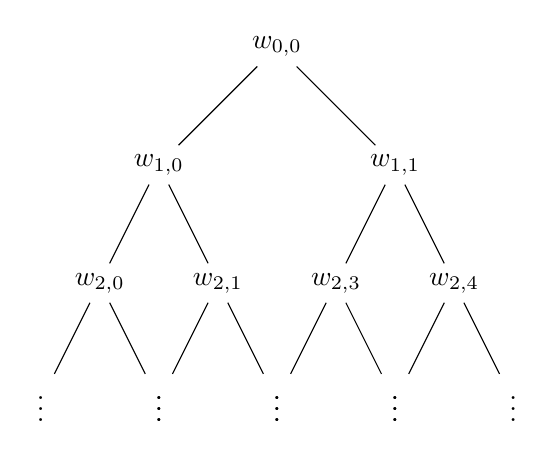
\begin{tikzpicture}[level distance=1.5cm,
  level 1/.style={sibling distance=3cm},
  level 2/.style={sibling distance=1.5cm}]
  \node {$w_{0,0}$}
    child {node {$w_{1,0}$}
      child {node {$w_{2,0}$}
      	child {node {\vdots}}
      	child {node {\vdots}}
      	}
      child {node {$w_{2,1}$}
      	child {node {\vdots}}
      	child {node {\vdots}}
      	}
    }
    child {node {$w_{1,1}$}
   	 child {node {$w_{2,3}$}
      child {node {\vdots}}
      child {node {\vdots}}
      }
    child {node {$w_{2,4}$}
      	child {node {\vdots}}
      	child {node {\vdots}}
      	}
    };      

\end{tikzpicture}
\end{center}
\caption{Binary wavelet tree for a one-dimensional signal. The nodes represent the large wavelet coefficients that arise from the discontinuities in smooth piecewise signals. The support of the large coefficients forms a rooted, connected tree.
}
\label{fig:ModelTree}
\end{figure}

\newpage

\subsection{Model-Based Algorithm (CoSaMP)} 

As the title suggests, the model-based signal recovery algorithm is based on the CoSaMP algorithm. We can construct the model-based algorithm by replacing the best K-sparse approximation and 2K-sparse approximation step in CoSaMP with a best (K-Model)-sparse approximation instead.  This way, we search for $m_{K}$ subspaces of $\mathcal{M}_{K}$ which is notably fewer than $\binom nk $ subspaces of $\sum_{K}$ in the CoSaMP recovery algorithm. 

The following theorem sets an upper bound for the error when experimenting with model sparse signals:

\newtheorem*{UB}{Theorem}
\begin{UB}
Let $\textbf{x} \in \mathcal{M}_{K}$ and let \textbf{b = Ax} + $\pmb{\eta}$ where $\textbf{x},\pmb{\eta},  \in \mathbb{R}^{N \times 1}$, $\textbf{b}\in \mathbb{R}^{M \times 1}$ and $\textbf{A} \in \mathbb{R}^{M \times N}$ be a set of noisy compressed sensing measurements. Then if, \textbf{A} has an $\mathcal{M}^{4}_{K}$-RIP constant of
 $\delta_{\mathcal{M}_{K}^{4}} \leq 0.1$, then the signal estimate $\hat{\textbf{x}}$ obtained at iteration i of the model based CoSaMP algorithm satisfies: 
 \begin{equation}
\begin{gathered}
||\textbf{x} - \hat{\textbf{x}}||_2 \leq 2^{-i} ||\textbf{x}||_2 + 15||\pmb{\eta}||_2. 
\end{gathered}
\label{eqn:UB}
\end{equation}
\end{UB}
Figure~\ref{fig:ModelReconstruct} shows the model-based signal reconstruction algorithm in action. 


\begin{figure}[H]
\centering
\includegraphics[scale=0.4]{Model.png}
\caption{An example of a Model-Based reconstruction and the usual CoSaMP reconstruction. The left-most image is the original image with $n = 128 \times 128$ pixels. The images to the right were recovered taking M = 5000 measurements with the picture in the middle representing the usual CoSaMP reconstruction and the right-most image is the reconstruction attempt using Model-Based recovery(Images taken from: \cite{MBCS})}
\label{fig:ModelReconstruct}
\end{figure}


\newpage

The algorithm for the CoSaMP variant of a Model-Based reconstruction algorithm is shown below. 


\begin{algorithm}
  \caption{Model Based CoSaMP}
  \bigskip	
  \textbf{Inputs}% Inputs section
  \begin{algorithmic}[1]
    \State Measurement matrix $\textbf{A} \in \mathbb{R}^{M \times N}$
    \State Output signal vector $\textbf{b} \in \mathbb{R}^{M \times 1}$
    \State K the sparsity of the original signal \textbf{x}
    \State A model $\mathcal{M}_K$
  \end{algorithmic}
  \bigskip  
  \textbf{Outputs}%
  \begin{algorithmic}[1]
    \State Signal $\hat{\textbf{x}} \in \mathbb{R}^{N \times 1}$ where $\hat{\textbf{x}}$ is K-sparse and is attuned to the model $\mathcal{M}_K$ given $\textbf{b} = \textbf{A}\hat{\hat{\textbf{x}}}$
  \end{algorithmic}
  \bigskip
  \textbf{Steps}% Steps section
  \begin{algorithmic}[1]
   \Procedure{MBCoSaMP}{$A,b,K,M$}
	\State $\textbf{x}^{(0)} \gets 0$
	\State $\textbf{v} \gets \textbf{b}$
	\State $i \gets 0$
   \While{Halting Criterion False}
    \State $i \gets i + 1$
	\State $z \gets \textbf{A}^{T}v$ \Comment{Signal Proxy}
    \State $\Omega \gets supp(\mathbb{M}_2 (\textbf{z},K))$\Comment{Support of residual approximation}
    \State $I \gets \Omega \cup supp(\textbf{x}^{(i - 1))}$\Comment{Augment Index Set}
    \State $\textbf{u}|_{I} \gets \textbf{A}_{I}^{\dagger}\textbf{b}; \quad \textbf{u}|_{I^{c}} \gets 0$ \Comment{Solve least squares}
    \State $\textbf{x}^{(i)} \gets \mathbb{M}(\textbf{u},K)$\Comment{Prune according to Model}
    \State $ \textbf{v} \gets \textbf{b} - \textbf{A}\textbf{x}^{(i)}$\Comment{Update Residual}
   \EndWhile
   
   \State $\textbf{return} \quad \hat{\textbf{x}} \gets \textbf{x}^{(i)}$
   \EndProcedure

  \end{algorithmic}
  
  \end{algorithm}



\newpage





\section{The Criterion for our Algorithms}\label{criterion}
Overall, to select the best algorithm, they must all be measured against certain criteria which I will define as follows:

\begin{itemize}
\item[1] The number of samples M needed for a given sparsity K to achieve accurate reconstruction. 

\item[2] The speed of the algorithm. 

\item[3] The algorithms accuracy and recovery rate including those perturbed by noise. 

\item[4] The applicability of the algorithm to all K-sparse signals. 

\end{itemize}

The first criterion is relatively easy to test for by comparing the recovery rates with fixed values for the sparsity of each algorithm. 

The second criterion similarly is accomplished through numerical tests and comparing algorithm run-times. However, a division of the results could be made so that you could identify algorithms which are fastest for datasets of a certain size. You could then determine which algorithm is the most reliable given the first criterion and comparing their logarithmic running time. 

A third criterion to compare each algorithm would be its ability to reconstruct the vector with the lowest amount of error possible given the measured data. This allows you to see, if in the general case of an MRI scan with noise, which algorithm is able to reconstruct the MRI image with a large degree of likeness (or the least amount of discernible differences).

The fourth criteria requires testing to be done on many K-sparse signals and analysing the performance on each K-sparse signal as the number of measurements increase. 

To conclude, there are many criterion for which you can compare algorithms and I will be using some of the above in my analysis. Each algorithm may be better suited to each task based on its properties whether its speed of reconstruction, accuracy or applicability for any level of sparsity or measurements. In my conclusion, I will measure the algorithms against this set criteria. 

\newpage




\newpage


\chapter{Reconstruction Algorithms}

\section{Goals and Approaches}

As a quick recap, we want to reconstruct a K-sparse signal $\textbf{x} \in \mathbb{R}^{N \times 1}$ from our sample output signal $\textbf{b} = \textbf{Ax} \in \mathbb{R}^{M \times 1}$. Given $\textbf{A} \in \mathbb{R}_{M \times N}$ and $M < N$, the system is undetermined as we have more unknowns than equations. We may have infinite solutions \textbf{z} for the original input signal \textbf{x}, however, as our assumption is that \textbf{x} is K-sparse, we can find a sufficient approximation to \textbf{x} from \textbf{b}. One of the most simple ways to recover such a vector from \textbf{ b = Ax} is by finding the sparsest vector (the one that has the most zero coefficients). 

We have that a vector \textbf{x} is K-sparse if:


\begin{equation}
\begin{gathered}
\textbf{x} \in \mathbb{R}^{N \times 1}, \quad ||\textbf{x}||_{0} = |supp(\textbf{x})| \leq K << N,
\end{gathered}
\label{eqn:sparse}
\end{equation}

where $||\cdot||_{0}$ is a vector norm. We can define other norms, formally known as p-norms as  $||\cdot||_{p}$ with $1 \leq p < \infty$


\begin{equation}
\begin{gathered}
\textbf{x} \in \mathbb{R}^{N \times 1}, \quad ||\textbf{x}||_{p} = (\sum_{i = 1}^{N}|x_{i}|^{p})^{1/p}, 
\end{gathered}
\label{eqn:pnorm}
\end{equation}

as well as

\begin{equation}
\begin{gathered}
\textbf{x} \in \mathbb{R}^{N \times 1}, \quad ||\textbf{x}||_{\infty} = \max |x_{i}|. 
\end{gathered}
\label{eqn:infnorm}
\end{equation}



The $\ell_{0}$ norm counts the number of non-zero coefficients and, so we try to find the smallest possible norm of the our approximation to the input signal \textbf{x} that satisfies this. the $\ell_{0}$-minimization problem as follows:

\begin{equation}
\begin{gathered}
\underset{\textbf{z} \in \mathbb{R}^{N \times 1}}{\min ||\textbf{z}||_{0}} \quad \text{subject to} \quad \textbf{b} = \textbf{Az}. 
\end{gathered}
\label{eqn:l0}
\end{equation}

Therefore, if the minimizer of~\ref{eqn:l0} is \textbf{z}, then we must have that \textbf{z = x}. The $\ell_{0}$-minimization problem in~\ref{eqn:l0}, which works perfectly well in theory, is non-deterministic polynomial-time hard (NP-Hard) in general\cite{DS:A&A}. The problem is too computationally intensive for any measurement matrix \textbf{A} and output signal \textbf{b}. However there are other ways to solve a similar problem to~\ref{eqn:l0} through lineary programming or greedy pursuits\cite{GP}, some of which are listed below:


\begin{itemize}
\item[1] Basis Pursuit (BP)\cite{BP-Atomic}.

\item[2] Orthogonal Matching Pursuit (OMP)\cite{GP-Orthog}.

\item[3] Regularized Orthogonal Matching Pursuit (ROMP) \cite{ROMP1}\cite{ROMP2}.

\item[4] Compressive Sampling Matching Pursuit (CoSaMP).\cite{CoSaMP}.

\item[5] Others such as StOMP\cite{STOMP} or Threshold methods\cite{ItThresh}.
 
\end{itemize}

Whether we solve the optimization problem through linear programming or utilize greedy algorithms, both types of algorithms have their advantages and disadvantages which will be discussed next after our initial numerical experiments on MRI images.  

The first algorithm which I will discuss is called Basis Pursuit or otherwise known as, $\ell_1$-minimization which utilizes linear programming to solve a similar problem to~\ref{eqn:l0}.

For practical purposes, algorithms used in compressive sensing must be relatively fast in their reconstruction of a signal. 
As previously established, the time taken to produce high-resolution images can range between several minutes to multiple hours. As a result, the speed of a reconstruction algorithm is one of the biggest reasons why research in this area has been growing at a rapid pace and so is an important criterion for which the algorithms are test on.

\newpage
\section{Basis Pursuit}\label{BP-Intro}
As established earlier, the $\ell_{0}$ problem in equation~\ref{eqn:l0} is an NP-Hard problem to recover the signal \textbf{x}. This NP-hard problem, however, for certain matrices\cite{UPSR} $\textbf{A} \in \mathbb{R}^{M \times N}$ we can perfectly recover K-sparse and noise free signals stably and approximate the compressible signal with large probability given $M = \mathcal{O}(KLog(N/K))$ identically distributed Gaussian measurements. Further the problem becomes equivalent to:

\begin{equation}
\begin{gathered}
\underset{\textbf{x} \in \mathbb{R}^{N \times 1}}{\min ||\textbf{x}||_{1}} \quad \text{subject to} \quad \textbf{b} = \textbf{Ax}. 
\end{gathered}
\label{eqn:l1}
\end{equation}


The programs~\ref{eqn:l0} and~\ref{eqn:l1}, are equivalent as proven by Candes and Tao\cite{delin}. An illustration of $\ell_{1}$ minimization is show in figure~\ref{fig:L1Tik}.

\begin{figure}[H]
\centering
\begin{tikzpicture}

\draw[thick,->] (0,0) -- (4.5,0);
\draw[thick,->] (0,0) -- (0,4.5);
\draw[thick,->] (0,0) -- (-4.5,0);
\draw[thick,->] (0,0) -- (0,-4.5);

\draw (0,1) -- (1,0);
\draw (0,-1) -- (1,0);
\draw (0,-1) -- (-1,0);
\draw (0,1) -- (-1,0);

\coordinate (centre) at (0,0);
\path (0,1) coordinate (A);

\fill[black] (A) circle[radius=4pt] node[left, xshift = -0.2cm]{$\textbf{z}$};

\draw[black] (A) -- ($(A)!4!-125:(centre)$);
\draw[black] (A) -- ($(A)!4!55:(centre)$) node[below, xshift = 1cm]{$\textbf{Ax = b}$};

%\pmb{SF}\textbf{x} + \pmb{\eta} = \textbf{b}.
%\pmb{\Phi}

\end{tikzpicture}
\caption{Here \textbf{x} is recovered exactly from \textbf{Ax = b} via $\ell_{1}$-minimization and \textbf{z = x}}
\label{fig:L1Tik}
\end{figure}


\newpage 

For measurement matrices that satisfy the restricted isometry property as detailed in chapter 2, Basis Pursuit is able to achieve exact recover all sparse signals as showned by Candes and Tao\cite{delin}. The following theorems  define the  conditions for exact sparse recovery along side theorems describing the stability of BP. 


\newtheorem*{ESR}{Theorem: Exact Sparse Recovery under RIP}
\begin{ESR}
Assume that a measurement matrix \textbf{A} satisfies the restricted isometry property. Then given that \textbf{A}'s isometry constants obey: 

\begin{equation}
\begin{gathered}
\delta_K + \delta_{2K} + \delta_{3K} < 1, 
\end{gathered}
\label{eqn:ESR}
\end{equation}
then any K-sparse signal \textbf{x} can be recovered exactly given its unique solution from~\ref{eqn:l1}. 
\end{ESR}

Furthermore, these guarantees are uniform. Once a measurement matrix satisfies the restricted isometric property, Basis Pursuit is able to correctly recover all sparse signals.

A more realistic scenario is where our measurements are noisy and the signal is not exactly sparse. Both the signals and the measurements are usually noisy and so we seek a solution that permits these conditions. The program in~\ref{eqn:l1} is not an appropriate meathod as the equality is not likely to be attainable. However, it has been shown that Basis pursuit is able to recover an approximation to noisy signals\cite{SSR}. We are able to modify the method to be able to account for some unknown perturbations. We can denote this perturbation as a signal vector $\pmb{\eta}$ which is bounded by some amount E i.e. $||\pmb{\eta}||_2 \leq E$  and we can denote our noisy observation as $\textbf{b = Ax} + \pmb{\eta}$.  
Further, small changes our observation of a signal, due to noise, should result in a small change in the recovery of the signal meaning that the method should be stable. We can denote the method as follows: 
\begin{equation}
\begin{gathered}
\underset{\textbf{x} \in \mathbb{R}^{N \times 1}}{\min ||\textbf{x}||_{1}} \quad \text{subject to} \quad ||\textbf{Ax} - \textbf{b}||_2 \leq E. 
\end{gathered}
\label{eqn:l1Quad}
\end{equation}
An illustration of this program is given by figure~\ref{fig:L1NoiseTik}


\begin{figure}[t]
\centering
\begin{tikzpicture}

\draw[thick,->] (0,0) -- (4.5,0);
\draw[thick,->] (0,0) -- (0,4.5);
\draw[thick,->] (0,0) -- (-4.5,0);
\draw[thick,->] (0,0) -- (0,-4.5);

\draw (0,1) -- (1,0);
\draw (0,-1) -- (1,0);
\draw (0,-1) -- (-1,0);
\draw (0,1) -- (-1,0);

\coordinate (centre) at (0,0);
\path (0,1) coordinate (A);
\path (0,1.5) coordinate (B);
\path (0,2) coordinate (C);

\fill[black] (A) circle[radius=4pt] node[left, xshift = -0.2cm]{$\textbf{z}$};
\fill[black] (C) circle[radius=4pt] node[right, xshift = 0.2cm]{$\textbf{x}$};

\draw[red] (A) -- ($(A)!4!-125:(centre)$);
\draw[red] (A) -- ($(A)!4!55:(centre)$);

\draw[black] (B) -- ($(B)!2.66666!-125:(centre)$);
\draw[black] (B) -- ($(B)!2.66666!55:(centre)$) node[below, xshift = 2cm]{$||\textbf{Ax - b}|| \leq E$};

\draw[red] (C) -- ($(C)!2!-125:(centre)$);
\draw[red] (C) -- ($(C)!2!55:(centre)$);


%\pmb{SF}\textbf{x} + \pmb{\eta} = \textbf{b}.
%\pmb{\Phi}

\end{tikzpicture}

\caption{An illustration of the reconstruction of a sparse signal \textbf{x} approximately from noisy data (\textbf{b} = \textbf{Ax} + \pmb{$\eta$}) where \pmb{$\eta$} is assumed to have a norm less than some error E.}
\label{fig:L1NoiseTik}

\end{figure}

The following theorems show that the program is able to recover a sparse signal with an error that's proportional to the noise level\cite{SSR}.

\newpage

\newtheorem*{Stab}{Theorem: Noisy Signal Recovery Bound}
\begin{Stab}
Assume that a measurement matrix \textbf{A} satisfies the restricted isometry property.  Further, given K, assume the isometry constants obey $\delta_{3K} + 3\delta_{4K} < 2$. Then for any K-sparse signal \textbf{x} with perturbation  $\pmb{\eta}$ with $||\pmb{\eta}||_2 \leq E$, there is a solution \textbf{z} such that: 
\begin{equation}
\begin{gathered}
||\textbf{z} - \textbf{x}||_2 \leq C_K \cdot E, 
\end{gathered}
\label{eqn:NSRB}
\end{equation}
where $C_K$ can only depend on $\delta_{4k}$. 
\end{Stab}

This theorem is consistent with the noiseless case given in~\ref{eqn:ESR}. Further, the majority of the singular values of the measurement matrix \textbf{A} is 0. This is because \textbf{A} is a rectangular matrix with fewer rows than columns. As a result, even though the problem is ill-posed, the error is controlled.
In addition, the condition in equation~\ref{eqn:ESR} is optimal for perturbations of size E. To show this, assume that the knowledge of the $supp(\textbf{x})$ prior to computation. Then, the most optimal way to reconstruct the signal \textbf{x} would be to make use of the least-squares method. Let \textbf{z} be the approximation to the original signal, then:


\begin{equation}
\begin{gathered}
\textbf{z}=
  \begin{cases}
    A_{K}^{\dagger}b, &\text{on supp(\textbf{x})}.\\
    0, & \text{elsewhere}.
  \end{cases}
\end{gathered}
\label{eqn:SBP-Cond}
\end{equation}

It is obvious that the error of $||\textbf{z} - \textbf{x}||_2 = 0$ on the complement of the $supp(\textbf{x})$ where as the error on the support is given by: $||\pmb{\eta}||_2 \leq E$. As a result, the best case scenario for the reconstruction of the signal is for it to have an error of which the size is proportional to the noise level.   

The following theorem shows stable recovery of all sparse vectors is possible\cite{SSR}.

\newtheorem*{Stab2}{Theorem: Stability of Basis Pursuit}
\begin{Stab2}
Assume that a measurement matrix \textbf{A} satisfies the restricted isometry property. Let $\textbf{x}_K$ denote the vector of the largest coefficients of \textbf{x}. Then for any K-sparse noisy signal $\textbf{b} = \textbf{Ax} + \pmb{\eta}$ with perturbation  with $||\pmb{\eta}||_2 \leq E$, the solution  \textbf{z} to~\ref{eqn:l1Quad} satisfies: 
\begin{equation}
\begin{gathered}
||\textbf{z} - \textbf{x}||_2 \leq C_K \cdot E + C_K^{T} \cdot \dfrac{||x - x_{K}||_1}{\sqrt{K}}.
\end{gathered}
\label{eqn:SBP2}
\end{equation}

\end{Stab2}

The theorem states that Basis Prusuit stabely recovers the K-largest entries of some signal \textbf{x}. 

To conclude, we now know that Basis Pursuit can exactly recover noiseless sparse signals and recovery of noisy signals is stable. 

\newpage

\subsection{Algorithm}

The algorithm is given as follows:

\begin{algorithm}
  \caption{Basis Pursuit via Dual Point Algorithm}
  \bigskip	
  \textbf{Inputs}% Inputs section
  \begin{algorithmic}[1]
   \State Measurement matrix $\textbf{A} \in \mathbb{R}^{M \times N}$
   \State Output signal vector $\textbf{b} \in \mathbb{R}^{M \times 1}$
  \end{algorithmic}
  \bigskip  
  \textbf{Outputs}%
  \begin{algorithmic}[1]
    \State A K-sparse Signal $\textbf{x}\in \mathbb{R}^{N \times 1}$ which satisfies $\textbf{b} = \textbf{A}\textbf{x}$
  \end{algorithmic}
  \bigskip
  \textbf{Steps}% Steps section
  \begin{algorithmic}[1]
   \Procedure{BP}{$A,b$}
\State $\textbf{z} \gets 0$
   \State $\textbf{v} \gets \textbf{A}^{T}\textbf{b}$  \Comment{Initial Guess}
   \State $\textbf{z} \gets \mathcal{DP}(\textbf{v},\textbf{A},\textbf{b})$ \Comment{Dual Point Method (L1 Magic)} 
   \State $\textbf{return} \quad \textbf{x} \gets \textbf{z}$
   \EndProcedure
   \end{algorithmic}

   \end{algorithm}
   
    The key to this algorithm is clearly the function $\mathcal{DP}$ and a detailed breakdown of the function is available online\cite{L1Magic}.

\newpage

\subsection{1D Signal - Basis Pursuit}

The following example makes used of $\ell_1-$Magic\cite{L1Magic} for the implementation of Basis Pursuit. We begin by creating a sparse-time signal. The signal shown in figure~\ref{fig:1DO}. 

The code is available in the appendix and the following graphs were generated with the following parameters:

\begin{itemize}
\item Signal Length (N) = 256.
\item Measurements (M) = 64. 
\item Sparsity/Peaks (K) = 20.
\item rng(10) (A random number seed to replicate results)
\end{itemize}

We measure the quality of the reconstruction via PSNR which is the Peak-Signal-to-Noise Ratio. PSNR is defined as follows:

\begin{equation}
\begin{gathered}
PSNR = 10 \cdot log_{10} \bigg(\dfrac{MAX_I^2}{MSE} \bigg), 
\end{gathered}
\end{equation}
where I is an $M \times N $ matrix. MAX is the maximum component of the signal and the Mean Squared Error (MSE) is given by: 

\begin{equation}
\begin{gathered}
MSE =  \dfrac{1}{N} \sum_{i=1}^{N} (\textbf{z} - \textbf{x})^2 ,
\end{gathered}
\end{equation}
where \textbf{z} and \textbf{x} vectors of length N. As the value of the PSNR grows larger, the better the recovery performance. A low PSNR value indicates a low-quality reconstruction. We also display the $\ell_2$-norm between the output and input signal on each graph. 


\begin{figure}[H]
\centering
\centerline{\includegraphics[scale=1]{OSignal.png}}
\caption{The plot of the (N = 256) original signal \textbf{x} with 20 peaks}
\label{fig:1DO}
\end{figure}

We then obtain 64 samples of the original signal as shown in the below figure:

\begin{figure}[H]
\centering
\centerline{\includegraphics[scale=1]{KVals.png}}
\caption{The plot of the (M = 64) signal generated by \textbf{Ax}}
\label{fig:1DK}
\end{figure}

We perform the Basis Pursuit algorithm and print the reconstructed signal along with its PSNR and 2-norm error:

\begin{figure}[H]
\centering
\centerline{\includegraphics[scale=1]{RSignal.png}}
\caption{The plot of the (N = 256) signal reconstructed via $\ell_1$-minimization}
\label{fig:1DR}
\end{figure}

Using only 64 samples taken using a measurement matrix with  Guassian random variables  as its entries, we recovered the 20-sparse original signal with a PSNR of 19.86. Taking a larger amount of samples of the same signal would results in a large PSNR i.e. a more accurate reconstruction of the original signal. Keeping the amount of samples constant and increasing the sparsity, meaning more zero coefficients in the signal, would have also increased the PSNR of the reconstruction when compared to the original. 


\newpage
\subsection{1D Signal - Basis Pursuit and Noisy Signals}

This section details the effect of noise and how the BP algorithm copes. As such, the equations which the signal follows is listed here:

\begin{equation}
\begin{gathered}
\underset{\textbf{x} \in \mathbb{R}^{N \times 1}}{\min ||\textbf{x}||_{1}} \quad \text{subject to} \quad ||\textbf{Ax} - \textbf{b}||_2 \leq E. 
\end{gathered}
\label{eqn:l1Quad2}
\end{equation}
Figures~\ref{fig:1DONoise} to \ref{fig:1DRNoiseF} show an example of a noise perturbed signal. The code of the for the below graphs can be located in the appendix. The quadratically constrained version of BP is needed to reconstruct a signal from a noisy observation. We again make use of $\ell_1$-Magic  to compute the solution. 

Figure~\ref{fig:1DONoise} shows the original signal  constructed. Notice how this signal is not sparse and as such, needs to be transformed into a sparse domain before we can compute its reconstruction using BP. 

\begin{figure}[H]
\centering
\centerline{\includegraphics[scale=0.6]{OSignalNoise.png}}
\caption{The plot of the (N = 1024) original signal \textbf{x}}
\label{fig:1DONoise}
\end{figure}

We can transform the signal into to the Discrete Cosine Transform (DCT).

\begin{figure}[H]
\centering
\centerline{\includegraphics[scale=0.5]{OSignalNoiseF.png}}
\caption{The plot of the Discrete Cosine Transform (DCT) coefficients for the (N = 1024) original signal. Notice how the majority of the coefficients are approximately 0. }
\label{fig:1DONoiseF}
\end{figure}
Given that our signal under DCT is sparse, we are able to apply the BP algorithm to the DCT coefficients of the signal. We can easily find the coefficients of corresponding sinusoid components and these coefficients (in the frequency domain) are shown in figure~\ref{fig:1DONoiseF}.  Figure~\ref{fig:1DKValsNoise} shows the 200 samples taken of the signal in the time domain as opposed to the frequency domain where we can find the DCT coefficients. 

\begin{figure}[H]
\centering
\centerline{\includegraphics[scale=0.5]{KValsNoise.png}}
\caption{The plot of the (M = 200) signal generated by $\textbf{A*x} +\pmb{\eta}$ where $\pmb{\eta}$ is some error vector. }
\label{fig:1DKValsNoise}
\end{figure}

Figure~\ref{fig:1DRNoise} shows the reconstruction of the original signal from 200 samples. Figure~\ref{fig:1DRNoiseF} shows the coefficients of the DCT of the reconstructed signal.  

\begin{figure}[H]
\centering
\centerline{\includegraphics[scale=0.5]{RSignalNoise200.png}}
\caption{The reconstructed signal (N = 1024) from (M = 200) the output vector  $\textbf{Ax} +\pmb{\eta}$ where $\pmb{\eta}$ is some error vector}
\label{fig:1DRNoise}
\end{figure}

\begin{figure}[H]
\centering
\centerline{\includegraphics[scale=0.5]{RSignalNoiseF.png}}
\caption{The plot of the Discrete Cosine Transform (DCT) coefficients for the (N = 1024) reconstructed signal.}
\label{fig:1DRNoiseF}
\end{figure}
\newpage

We can see why the PSNR is low visually and similarly for the error. From this, I generate 4 more figures~\ref{fig:1DRNoise400} to \ref{fig:1DRNoise1000} to demonstrate the effect of an increasing number of measurements on the time taken to reconstruct the signal, the PSNR of the reconstruction and the 2-Norm error

\begin{figure}[H]
\centering
\centerline{\includegraphics[scale=0.5]{RSignalNoise200.png}}
\caption{The reconstruction of the original signal (N = 1024) using 200 measurements}
\label{fig:1DRNoise200}
\end{figure}

\begin{figure}[H]
\centering
\centerline{\includegraphics[scale=0.5]{RSignalNoise400.png}}
\caption{The reconstruction of the original signal (N = 1024) using 400 measurements}
\label{fig:1DRNoise400}
\end{figure}

\begin{figure}[H]
\centering
\centerline{\includegraphics[scale=0.6]{RSignalNoise600.png}}
\caption{The reconstruction of the original signal (N = 1024) using 600 measurements}
\label{fig:1DRNoise600}
\end{figure}

\begin{figure}[H]
\centering
\centerline{\includegraphics[scale=0.6]{RSignalNoise800.png}}
\caption{The reconstruction of the original signal (N = 1024) using 800 measurements}
\label{fig:1DRNoise800}
\end{figure}

\begin{figure}[H]
\centering
\centerline{\includegraphics[scale=0.6]{RSignalNoise1000.png}}
\caption{The reconstruction of the original signal (N = 1024) using 1000 measurements}
\label{fig:1DRNoise1000}
\end{figure}

The above figures clearly show that as we take more measurements and execute the BP algorithm, the PSNR of the reconstructed signal increases and continually becomes more similar to the original signal presented in figure ~\ref{fig:1DONoise}. The time taken for the execution of the algorithm  fluctuates between 1.1 and 1.4 seconds and the 2-Norm also continually decreases as we take more measurements. 

To conclude, Basis Pursuit is able to reconstruct signals from noisy observations to a high accuracy. As shown earlier, however, the resulting signal 2-norm error is bounded by the 2-norm of the error vector. 


\newpage
\subsection{1D Signal - Basis Pursuit Numerical Results}

The code for the graphs in this section are found in the appendix. In every case, the measurement matrix used was a Gaussian matrix and the graphs were all produced using MATLAB. Outside functions used include: $\ell_1$-Magic\cite{L1Magic}. 

This first graph was generated by running my code for the given parameters:

\begin{itemize}
\item[1] Sample measurements ranging from 1 to 100.
\item[2] Sparsity levels ranging from 5 to 30. 
\end{itemize}

For each point on the graph, 100 values were taken and averaged to represent the data point. Figure~\ref{fig:1DSNR} shows the relationship between the measurements M and the sparsity K and their effect on the PSNR of the reconstructed signal. We can clearly see that as the number of measurements increase, so does the PSNR of the reconstructed signal. Further, as the sparsity of signal decreases, the lower the PSNR of the reconstructed image. We can see that, for example, at 50 measurements the PSNR for the reconstruction of a 15-sparse signal is approximately 40dB. As the signal gains more non-zero values, the PSNR decreases as shown for K = 30 where the PSNR is approximately 10dB. If the sparsity of the signal was to increase to say, K = 10, we can see that the PSNR of the reconstructed signal jumps to approximately 90dB. For our given measurements, the graphs seem to approach a limit at a point below 140dB. From this we can conclude that there exists a point where the computational cost of reconstructing an image from a large number of measurements is too large for the increase in PSNR achieved by doing so unless there exists another large "jump" as seen for every sparsity level measured. 



\begin{figure}[H]
\centering
\centerline{\includegraphics[scale=0.75]{PSNRTrend.png}}
\caption{Plot of how PSNR values change for a N = 256 dimensional signal with increasing samples (1 to 100 in steps of 1) and 6 levels of sparsity (5 to 30 in steps of 5). The output is the average of 100 trials that were run for each combination of the number of samples and sparsity.}
\label{fig:1DSNR}
\end{figure}


Figure~\ref{fig:1DError} shows the relationship between the measurements M and the sparsity K and their effect on the 2-Norm error of the reconstructed signal. Again, the effect is obvious as we can see that an increase in measurements coincides with the deprecation of the 2-Norm error value. The sparser the signal, the smaller the initial 2-Norm error and the faster that error decays as the number of measurements increases. We can approximate the gradient of the curves by finding the gradient of the line of best fit. For K = 5, we see that the error becomes approximately 0 at M = 35. We can approximate that at M =1, the error is 2.5 and as such, the gradient is approximately 0.071. For K = 15, the error is approximately 0 at 70 and we can assume that a line of best fit would coincide with error value 4.5. This gives a gradient of 0.064. From our results, we can conclude that the denser the signal is, the slower 2-norm error decays to 0. 


\begin{figure}[H]
\centering
\centerline{\includegraphics[scale=0.75]{ErrorTrend.png}}
\caption{Plot of how the 2-norm error values change for a N = 256 dimensional signal with increasing samples (1 to 100 in steps of 1) and 6 levels of sparsity (5 to 30 in steps of 5). The output is the average of 100 trials that were run for each combination of the number of samples and sparsity. Code for graph generation is available in Appendix~\ref{lst:ex1DGraphs}}
\label{fig:1DError}
\end{figure}

The graph in Figure~\ref{fig:1DCorrect} displays how many signals BP is able to correctly construct given the threshold that the 2-norm must be less than 0.01. For very sparse signals we can clearly see that the measurements required to achieve 100\% successful recovery is small i.e. K = 5 requires approximately 35 measurements. For the measurements and sparsity levels displayed, we notice that for an additional 5 non-zero values present in a signal, the amount of measurements required to achieve 100\% correct reconstruction increases by 20 i.e for K = 10, M = 55 which is 20 more than for K = 5. Our displayed results show that 100\% successful reconstruction is possible for $K \geq 5$ given that we take  $M \geq 20$ measurements more than those that were needed for a signal with 5 less non-zero values. Due to this constant, the ratio of measurements and sparsity for 100\% signal reconstruction decreases as the signal becomes more dense. 

\begin{figure}[H]
\centering
\centerline{\includegraphics[scale=0.75]{CRTrend.png}}
\caption{Plot of how the percentage of signals correctly recovered change for a N = 256 dimensional signal with increasing samples (1 to 100 in steps of 1) and 6 levels of sparsity (5 to 30 in steps of 5). The output is the average of 100 trials that were run for each combination of the number of samples and sparsity. Code for graph generation is available in Appendix~\ref{lst:ex1DGraphs}}
\label{fig:1DCorrect}
\end{figure}

\newpage

\section{MRI Images - Experiments}
I will perform my numerical experiments on the two MRI images and they will remain the same for BP, OMP and CoSaMP. However, due to data processing ability of my computer, every image will be of size $N = 80 \times 80$ in my experiments carried out. As a result the images are small and I've had to magnify them, however, the change is obvious to see in the majority of the cases I'll explore. These images need to be transformed into a sparse domain and to that end I threshold the largest 10\% of the values if the followings domains:

\begin{itemize}
\item Discrete Cosine Transform (Denoted: DCT)
\item Fourier Transform (Denoted: FFT)
\item Discrete Wavelet Transform (Denoted: DWT)
\end{itemize}  

The original MRI images are given below but the K-sampled images will be given for each of the transforms we perform.  

\begin{figure}[H]
\centering
\begin{subfigure}{.5\textwidth}
  \centering
  \includegraphics[width=100px,height=100px]{Brain-T2-axial.png}
  \caption{MRI - Brain 1 : T2-weighted MR image of a normal brain\cite{Brain1}.}
  \label{fig:Brain1}
\end{subfigure}%
\hspace*{2em}
\begin{subfigure}{.5\textwidth}
  \centering
  \includegraphics[width=100px,height=100px]{BrainImage.jpg}
  \caption{MRI - Brain 2: 3T MRI image of a human head with a pituitary tumour\cite{Brain2}.}
  \label{fig:Brain2}
\end{subfigure}
\caption{I will be using the following MRI scans to test the CS algorithms.}
\label{fig:MRIImages}
\end{figure}

\section{Basis Pursuit - Experiments}

\subsection{Brain 1 - Image Reconstruction}

I begin my numerical experiments on the MRI image~\ref{fig:Brain1}. Each column will represent the image produced from each transform which from left to right is: DCT, FFT, DWT. 

\begin{figure}[!h]
\centering
\minipage{0.32\textwidth}
  \includegraphics[width=\linewidth]{BP-Brain1-Original-DCT.png}
  \caption{DCT: Image K = 10\%}\label{fig:BP-Brain1-Original-DCT}
\endminipage
\hspace*{2em}
\minipage{0.32\textwidth}
  \includegraphics[width=\linewidth]{BP-Brain1-Original-FFT.png}
  \caption{FFT: Image K = 10\%}\label{fig:BP-Brain1-Original-FFT}
\endminipage
\hspace*{2em}
\minipage{0.32\textwidth}%
  \includegraphics[width=\linewidth]{BP-Brain1-Original-DWT.png}
  \caption{DWT: Image K = 10\%}\label{fig:BP-Brain1-Original-DWT}
\endminipage
\hspace*{2em}
\end{figure}

\begin{figure}[!h]
\centering
\minipage{0.32\textwidth}
  \includegraphics[width=\linewidth]{BP-Brain1-640-DCT.png}
  \caption{DCT: Image M = K = 640}\label{fig:BP-Brain1-640-DCT}
\endminipage
\hspace*{2em}
\minipage{0.32\textwidth}
  \includegraphics[width=\linewidth]{BP-Brain1-640-FFT}
  \caption{FFT: Image M = K = 640}\label{fig:BP-Brain1-640-FFT}
\endminipage
\hspace*{2em}
\minipage{0.32\textwidth}%
  \includegraphics[width=\linewidth]{BP-Brain1-640-DWT}
  \caption{DWT: Image M = K = 640}\label{fig:BP-Brain1-640-DWT}
\endminipage
\hspace*{2em}
\end{figure}

\begin{figure}[!h]
\centering
\minipage{0.32\textwidth}
  \includegraphics[width=\linewidth]{BP-Brain1-960-DCT.png}
  \caption{DCT: Image M = 1.5K = 960}\label{fig:BP-Brain1-960-DCT}
\endminipage
\hspace*{2em}
\minipage{0.32\textwidth}
  \includegraphics[width=\linewidth]{BP-Brain1-960-FFT}
  \caption{FFT: Image M = 1.5K = 960}\label{fig:BP-Brain1-960-FFT}
\endminipage
\hspace*{2em}
\minipage{0.32\textwidth}%
  \includegraphics[width=\linewidth]{BP-Brain1-960-DWT}
  \caption{DWT: Image M = 1.5K = 960}\label{fig:BP-Brain1-960-DWT}
\endminipage
\hspace*{2em}
\end{figure}

\clearpage
\begin{figure}[!h]
\centering
\minipage{0.32\textwidth}
  \includegraphics[width=\linewidth]{BP-Brain1-1280-DCT.png}
  \caption{DCT: Image M = 2K = 1280}\label{fig:BP-Brain1-1280-DCT}
\endminipage
\hspace*{2em}
\minipage{0.32\textwidth}
  \includegraphics[width=\linewidth]{BP-Brain1-1280-FFT}
  \caption{FFT: Image M = 2K = 1280}\label{fig:BP-Brain1-1280-FFT}
\endminipage
\hspace*{2em}
\minipage{0.32\textwidth}%
  \includegraphics[width=\linewidth]{BP-Brain1-1280-DWT}
  \caption{DWT: Image M = 2K = 1280}\label{fig:BP-Brain1-1280-DWT}
\endminipage
\hspace*{2em}
\end{figure}

\begin{figure}[!h]
\centering
\minipage{0.32\textwidth}
  \includegraphics[width=\linewidth]{BP-Brain1-1600-DCT.png}
  \caption{DCT: Image M = 2.5K = 1600}\label{fig:BP-Brain1-1600-DCT}
\endminipage
\hspace*{2em}
\minipage{0.32\textwidth}
  \includegraphics[width=\linewidth]{BP-Brain1-1600-FFT}
  \caption{FFT: Image M = 2.5K = 1600}\label{fig:BP-Brain1-1600-FFT}
\endminipage
\hspace*{2em}
\minipage{0.32\textwidth}%
  \includegraphics[width=\linewidth]{BP-Brain1-1600-DWT}
  \caption{DWT: Image M = 2.K = 1600}\label{fig:BP-Brain1-1600-DWT}
\endminipage
\hspace*{2em}
\end{figure}

\begin{figure}[!h]
\centering
\minipage{0.32\textwidth}
  \includegraphics[width=\linewidth]{BP-Brain1-1920-DCT.png}
  \caption{DCT: Image M = 3K = 1920}\label{fig:BP-Brain1-1920-DCT}
\endminipage
\hspace*{2em}
\minipage{0.32\textwidth}
  \includegraphics[width=\linewidth]{BP-Brain1-1920-FFT}
  \caption{FFT: Image M = 3K = 1920}\label{fig:BP-Brain1-1920-FFT}
\endminipage
\hspace*{2em}
\minipage{0.32\textwidth}%
  \includegraphics[width=\linewidth]{BP-Brain1-1920-DWT}
  \caption{DWT: Image M = 3K = 1920}\label{fig:BP-Brain1-1920-DWT}
\endminipage
\hspace*{2em}
\end{figure}

\clearpage

\begin{figure}[!h]
\centering
\minipage{0.32\textwidth}
  \includegraphics[width=\linewidth]{BP-Brain1-2240-DCT.png}
  \caption{DCT: Image M = 3.5K = 2240}\label{fig:BP-Brain1-2240-DCT}
\endminipage
\hspace*{2em}
\minipage{0.32\textwidth}
  \includegraphics[width=\linewidth]{BP-Brain1-2240-FFT}
  \caption{FFT: Image M = 3.5K = 2240}\label{fig:BP-Brain1-2240-FFT}
\endminipage
\hspace*{2em}
\minipage{0.32\textwidth}%
  \includegraphics[width=\linewidth]{BP-Brain1-2240-DWT}
  \caption{DWT: Image M = 3.5K = 2240}\label{fig:BP-Brain1-2240-DWT}
\endminipage
\hspace*{2em}
\end{figure}

\begin{figure}[!h]
\centering
\minipage{0.32\textwidth}
  \includegraphics[width=\linewidth]{BP-Brain1-2560-DCT.png}
  \caption{DCT: Image M = 4K = 2240}\label{fig:BP-Brain1-2560-DCT}
\endminipage
\hspace*{2em}
\minipage{0.32\textwidth}
  \includegraphics[width=\linewidth]{BP-Brain1-2560-FFT}
  \caption{FFT: Image M = 4K = 2560}\label{fig:BP-Brain1-2560-FFT}
\endminipage
\hspace*{2em}
\minipage{0.32\textwidth}%
  \includegraphics[width=\linewidth]{BP-Brain1-2560-DWT}
  \caption{DWT: Image M = 4K = 2560}\label{fig:BP-Brain1-2560-DWT}
\endminipage
\hspace*{2em}
\end{figure}

\begin{figure}[!h]
\centering
\minipage{0.32\textwidth}
  \includegraphics[width=\linewidth]{BP-Brain1-2880-DCT.png}
  \caption{DCT: Image M = 4.5K = 2880}\label{fig:BP-Brain1-2880-DCT}
\endminipage
\hspace*{2em}
\minipage{0.32\textwidth}
  \includegraphics[width=\linewidth]{BP-Brain1-2880-FFT}
  \caption{FFT: Image M = 4.5K = 2880}\label{fig:BP-Brain1-2880-FFT}
\endminipage
\hspace*{2em}
\minipage{0.32\textwidth}%
  \includegraphics[width=\linewidth]{BP-Brain1-2880-DWT}
  \caption{DWT: Image M = 4.5K = 2880}\label{fig:BP-Brain1-2880-DWT}
\endminipage
\hspace*{2em}
\end{figure}
\clearpage

\subsection{Brain 1 Image - Analysis}

Following the results, I generated some graphs showing how the time, error and PSNR changed as I increased the number of measurements and these graphs are shown below. The x-axis is labelled so that the measurements in each image is displayed as a multiple of the sparsity K of the original image. 

\begin{figure}[H]
\centering
\centerline{\includegraphics[scale=0.6]{BP-MRI-PSNR-Brain1.png}}
\caption{Plot of how the PSNR values change for an increasing number of measurements for Brain 1.}
\label{fig:BP-MRI-PSNR-Brain1}
\end{figure}

We immediately note that there is a problem with the FFT reconstruction of the image. This is due to the algorithm in $\ell_1$-Magic where the programs gets stuck backtracking in its line search and returns to its last successful iterations. As a result, all the images look similar and we aren't able to read too much into the results of FFT reconstructions. More informations is available about this in the relevant documentation for $\ell_1$-Magic.

As expected, however, the PSNR does increase, no matter how small as the number of measurements increases. The largest jump is see at M = 3.5K after which the signals shows a slow rise until stabilization to the maximum PSNR. The error in reconstruction behaves similar to that of the graph of the PSNR values with the biggest change in error to almost 0 is at M = 3.5K. The time taken to perform the algorithm on each transform is shown below with the wavelet transform being the fastest. In general, we see a slow rise in the time taken as M/K increases which is to be expected. 


\begin{figure}[H]
\centering
\centerline{\includegraphics[scale=0.6]{BP-MRI-Error-Brain1.png}}
\caption{Plot of how the error values change for an increasing number of measurements for Brain 1.}
\label{fig:BP-MRI-Error-Brain1}
\end{figure}

\begin{figure}[H]
\centering
\centerline{\includegraphics[scale=0.6]{BP-MRI-Time-Brain1.png}}
\caption{Plot of how the time to generate the results change for an increasing number of measurements for Brain 1.}
\label{fig:BP-MRI-Time-Brain1}
\end{figure}

\clearpage


\subsection{Brain 2 - Image Reconstruction}

I now run tests on image~\ref{fig:Brain2}. As before each column will represent the image produced from each transform which from left to right is: DCT, FFT, DWT. 

\begin{figure}[!h]
\centering
\minipage{0.32\textwidth}
  \includegraphics[width=\linewidth]{BP-Brain2-Original-DCT.png}
  \caption{DCT: Image K = 10\%}\label{fig:BP-Brain2-Original-DCT}
\endminipage
\hspace*{2em}
\minipage{0.32\textwidth}
  \includegraphics[width=\linewidth]{BP-Brain2-Original-FFT.png}
  \caption{FFT: Image K = 10\%}\label{fig:BP-Brain2-Original-FFT}
\endminipage
\hspace*{2em}
\minipage{0.32\textwidth}%
  \includegraphics[width=\linewidth]{BP-Brain2-Original-DWT.png}
  \caption{DWT: Image K = 10\%}\label{fig:BP-Brain2-Original-DWT}
\endminipage
\hspace*{2em}
\end{figure}

\begin{figure}[!h]
\centering
\minipage{0.32\textwidth}
  \includegraphics[width=\linewidth]{BP-Brain2-640-DCT.png}
  \caption{DCT: Image M = K = 640}\label{fig:BP-Brain2-640-DCT}
\endminipage
\hspace*{2em}
\minipage{0.32\textwidth}
  \includegraphics[width=\linewidth]{BP-Brain1-640-FFT}
  \caption{FFT: Image M = K = 640}\label{fig:BP-Brain2-640-FFT}
\endminipage
\hspace*{2em}
\minipage{0.32\textwidth}%
  \includegraphics[width=\linewidth]{BP-Brain2-640-DWT}
  \caption{DWT: Image M = K = 640}\label{fig:BP-Brain2-640-DWT}
\endminipage
\hspace*{2em}
\end{figure}

\begin{figure}[!h]
\centering
\minipage{0.32\textwidth}
  \includegraphics[width=\linewidth]{BP-Brain2-960-DCT.png}
  \caption{DCT: Image M = 1.5K = 960}\label{fig:BP-Brain2-960-DCT}
\endminipage
\hspace*{2em}
\minipage{0.32\textwidth}
  \includegraphics[width=\linewidth]{BP-Brain2-960-FFT}
  \caption{FFT: Image M = 1.5K = 960}\label{fig:BP-Brain2-960-FFT}
\endminipage
\hspace*{2em}
\minipage{0.32\textwidth}%
  \includegraphics[width=\linewidth]{BP-Brain2-960-DWT}
  \caption{DWT: Image M = 1.5K = 960}\label{fig:BP-Brain2-960-DWT}
\endminipage
\hspace*{2em}
\end{figure}

\clearpage
\begin{figure}[!h]
\centering
\minipage{0.32\textwidth}
  \includegraphics[width=\linewidth]{BP-Brain2-1280-DCT.png}
  \caption{DCT: Image M = 2K = 1280}\label{fig:BP-Brain2-1280-DCT}
\endminipage
\hspace*{2em}
\minipage{0.32\textwidth}
  \includegraphics[width=\linewidth]{BP-Brain2-1280-FFT}
  \caption{FFT: Image M = 2K = 1280}\label{fig:BP-Brain2-1280-FFT}
\endminipage
\hspace*{2em}
\minipage{0.32\textwidth}%
  \includegraphics[width=\linewidth]{BP-Brain2-1280-DWT}
  \caption{DWT: Image M = 2K = 1280}\label{fig:BP-Brain2-1280-DWT}
\endminipage
\hspace*{2em}
\end{figure}

\begin{figure}[!h]
\centering
\minipage{0.32\textwidth}
  \includegraphics[width=\linewidth]{BP-Brain2-1600-DCT.png}
  \caption{DCT: Image M = 2.5K = 1600}\label{fig:BP-Brain2-1600-DCT}
\endminipage
\hspace*{2em}
\minipage{0.32\textwidth}
  \includegraphics[width=\linewidth]{BP-Brain2-1600-FFT}
  \caption{FFT: Image M = 2.5K = 1600}\label{fig:BP-Brain2-1600-FFT}
\endminipage
\hspace*{2em}
\minipage{0.32\textwidth}%
  \includegraphics[width=\linewidth]{BP-Brain2-1600-DWT}
  \caption{DWT: Image M = 2.K = 1600}\label{fig:BP-Brain2-1600-DWT}
\endminipage
\hspace*{2em}
\end{figure}

\begin{figure}[!h]
\centering
\minipage{0.32\textwidth}
  \includegraphics[width=\linewidth]{BP-Brain2-1920-DCT.png}
  \caption{DCT: Image M = 3K = 1920}\label{fig:BP-Brain2-1920-DCT}
\endminipage
\hspace*{2em}
\minipage{0.32\textwidth}
  \includegraphics[width=\linewidth]{BP-Brain2-1920-FFT}
  \caption{FFT: Image M = 3K = 1920}\label{fig:BP-Brain2-1920-FFT}
\endminipage
\hspace*{2em}
\minipage{0.32\textwidth}%
  \includegraphics[width=\linewidth]{BP-Brain2-1920-DWT}
  \caption{DWT: Image M = 3K = 1920}\label{fig:BP-Brain2-1920-DWT}
\endminipage
\hspace*{2em}
\end{figure}

\clearpage

\begin{figure}[!h]
\centering
\minipage{0.32\textwidth}
  \includegraphics[width=\linewidth]{BP-Brain2-2240-DCT.png}
  \caption{DCT: Image M = 3.5K = 2240}\label{fig:BP-Brain2-2240-DCT}
\endminipage
\hspace*{2em}
\minipage{0.32\textwidth}
  \includegraphics[width=\linewidth]{BP-Brain2-2240-FFT}
  \caption{FFT: Image M = 3.5K = 2240}\label{fig:BP-Brain2-2240-FFT}
\endminipage
\hspace*{2em}
\minipage{0.32\textwidth}%
  \includegraphics[width=\linewidth]{BP-Brain2-2240-DWT}
  \caption{DWT: Image M = 3.5K = 2240}\label{fig:BP-Brain2-2240-DWT}
\endminipage
\hspace*{2em}
\end{figure}

\begin{figure}[!h]
\centering
\minipage{0.32\textwidth}
  \includegraphics[width=\linewidth]{BP-Brain2-2560-DCT.png}
  \caption{DCT: Image M = 4K = 2240}\label{fig:BP-Brain2-2560-DCT}
\endminipage
\hspace*{2em}
\minipage{0.32\textwidth}
  \includegraphics[width=\linewidth]{BP-Brain2-2560-FFT}
  \caption{FFT: Image M = 4K = 2560}\label{fig:BP-Brain2-2560-FFT}
\endminipage
\hspace*{2em}
\minipage{0.32\textwidth}%
  \includegraphics[width=\linewidth]{BP-Brain2-2560-DWT}
  \caption{DWT: Image M = 4K = 2560}\label{fig:BP-Brain2-2560-DWT}
\endminipage
\hspace*{2em}
\end{figure}

\begin{figure}[!h]
\centering
\minipage{0.32\textwidth}
  \includegraphics[width=\linewidth]{BP-Brain2-2880-DCT.png}
  \caption{DCT: Image M = 4.5K = 2880}\label{fig:BP-Brain2-2880-DCT}
\endminipage
\hspace*{2em}
\minipage{0.32\textwidth}
  \includegraphics[width=\linewidth]{BP-Brain2-2880-FFT}
  \caption{FFT: Image M = 4.5K = 2880}\label{fig:BP-Brain2-2880-FFT}
\endminipage
\hspace*{2em}
\minipage{0.32\textwidth}%
  \includegraphics[width=\linewidth]{BP-Brain2-2880-DWT}
  \caption{DWT: Image M = 4.5K = 2880}\label{fig:BP-Brain2-2880-DWT}
\endminipage
\hspace*{2em}
\end{figure}
\clearpage

\subsection{Brain 2 Image - Analysis}

The graphs below show how the time, error and PSNR changed as I increased the number of measurements. 

\begin{figure}[H]
\centering
\centerline{\includegraphics[scale=0.6]{BP-MRI-PSNR-Brain2.png}}
\caption{Plot of how the PSNR values change for an increasing number of measurements for Brain 2.}
\label{fig:BP-MRI-PSNR-Brain2}
\end{figure}

The second images suffers from the same problem in regards to the FFT reconstruction. However, we do note that the the image does visually become more clear as the ratio of M/K increases. 
Unsurprisingly, the results show the same trend as discussed in the analysis of the first brain. There may be small variance in the actual points in the graphs, but the overall trend remains the same and there is no large discernible difference. 


\begin{figure}[H]
\centering
\centerline{\includegraphics[scale=0.6]{BP-MRI-Error-Brain2.png}}
\caption{Plot of how the error values change for an increasing number of measurements for Brain 2.}
\label{fig:BP-MRI-Error-Brain2}
\end{figure}

\begin{figure}[H]
\centering
\centerline{\includegraphics[scale=0.6]{BP-MRI-Time-Brain2.png}}
\caption{Plot of how the time to generate the results change for an increasing number of measurements for Brain 2.}
\label{fig:BP-MRI-Time-Brain2}
\end{figure}

\clearpage

\section{Conclusion}

From our analysis and the theorems described earlier, it is obvious that $\ell_1$-minimization method, Basis Pursuit, has many advantages. Exact recovery of a sparse noiseless signal is possible when the condition specified in equation~\ref{eqn:ESR} is satisfied.  The method is also stable meaning given that a measurement matrix which satisfies the restricted isometric property, Basis Pursuit is able to reconstruct all K-sparse signals \textbf{x} ,noisy or noise-less, as demonstrated by equation~\ref{eqn:SBP2}. As a result of this, the guarantees provided are uniform meaning there are no failures in reconstructing any K-sparse signal. As described in the introduction in section~\ref{BP-Intro}, given  $M = \mathcal{O}(KLog(N/K))$ identically distributed Gaussian measurements, we can approximate a compressible signal with large probability.

Whilst Basis Pursuit provides uniform guarantees and is stable, it is based on linear programming which is known to have algorithms of polynomial run time and therefore, is slower than some of the greedier methods. 
However, the ability to reconstruct all sparse signals even those perturbed by noise means that the algorithm can be used as a method to solve many problems because of its applicability. 

\begin{flushleft}
To summarize:
\end{flushleft}

\textbf{Advantages}
\begin{itemize}
\item Provides uniform guarantees.
\item Is a stable algorithm.
\end{itemize}

\textbf{Disadvantages}
\begin{itemize}
\item Has slow, polynomial run time.
\end{itemize}

\newpage

\section{Orthogonal Matching Pursuit}
A brief introduction to how OMP works was given in section~\ref{OMP}. Following this, we can introduce a theorem developed by Tropp and Gilbert\cite{GP-Orthog} which shows that OMP can accurately reconstruct a K-sparse signal \textbf{x} from an M  measurements using a $M \times N$ subgaussian measurement matrix . 

\newtheorem*{SROMP}{Theorem: Sparse Recovery via OMP\cite{GP-Orthog}}\label{SROMPTH}
\begin{SROMP}
Fix $\delta \in (0,0.36)$ and choose $M \geq ZKlog\bigg(\dfrac{N}{\delta}\bigg)$. Suppose that $\textbf{x} \in \mathbb{R}^{N \times 1}$ is a K-sparse signal and let $\textbf{A} \in \mathbb{R}^{M \times N}$ be a measurement matrix with entries consisting of independent and identically distributed variables from the standard Gaussian distribution. Let $\textbf{b} \in \mathbb{R}^{M \times 1}$, then given \textbf{b = Ax}, the OMP algorithm is able to correctly reconstruct the K-sparse signal \textbf{x} with greater than $1 - 2\delta$ probability. The constant Z must satisfy $Z \leq 20$ and for large values of K, $Z \approx 4$. 

\end{SROMP}

Note, however, that this guarantee is weak as it is only for a fixed K-sparse signal \textbf{x}. As a result, OMP may fail for some K-sparse signals.

\bigskip
The iterative steps of the algorithm can be explained as follows:

\begin{itemize}
\item[1] \textbf{Identify:} Find the largest coefficient of the residual \textbf{r} where initially, (\textbf{r = b = Ax}), and retrieve its index and store it as $\lambda$. 

\item[2] \textbf{Augment:} Augment the initially empty index set $\pmb{\mathcal{I}}$ with the newly identified index $\lambda$. Also augment the initially empty matrix \textbf{A} with the column $\textbf{A}_{\lambda}$.

\item[3] \textbf{Estimate:} Retrieve an estimate for the original signal \textbf{x} by using least squares. We want to find the projection of \textbf{b}  on the range of the columns of \textbf{A}. 

\item[4] \textbf{Update:} Update the residual with its new value using the estimated signal \textbf{x}.


\end{itemize}
\newpage
\subsection{Algorithm}
The algorithm for OMP is given as follows: 

\begin{algorithm}[H]
  \caption{OMP Algorithm}
  \bigskip	
  \textbf{Inputs}% Inputs section
  \begin{algorithmic}[1]
    \State Measurement matrix $\textbf{A} \in \mathbb{R}^{M \times N}$.
    \State Output signal vector $\textbf{b} \in \mathbb{R}^{M \times 1}$.
    \State The number of iterations (K) to perform (K = Sparsity value of original signal $\textbf{x} \in \mathbb{R}^{N \times 1}$ ). 
  \end{algorithmic}
  \bigskip  
  \textbf{Outputs}%
  \begin{algorithmic}[1]
    \State A K-sparse Signal $\textbf{x}\in \mathbb{R}^{N \times 1}$ which satisfies $\textbf{b} = \textbf{A}\textbf{x}$.
     \State An index set $\pmb{\mathcal{I}}$ which holds the index of the non-zero values of \textbf{x}. 
      \State An estimation of the observation vector \textbf{b} via \textbf{y}. 
       \State The residual \textbf{r}. 
  \end{algorithmic}
  \bigskip
  \textbf{Steps}% Steps section
  \begin{algorithmic}[1]
   \Procedure{OMP}{$A,b,K$}
\State $\textbf{r}^{(0)} \gets \textbf{b}$
\State $i \gets 0$
   \State $\pmb{\mathcal{I}}^{(0)} \gets \emptyset$
   \While{$i \leq K$}
   \State $i \gets i + 1$
   \State $\lambda^{(i)} \gets arg \underset{j = 1,\hdots,N}\max |<\textbf{r}^{(i - 1)}, \textbf{A}_{j}>|$ \Comment{Get index of largest entry}
   \State $\pmb{\mathcal{I}}^{(i)} \gets \pmb{\mathcal{I}}^{(i-1)} \cup \lambda^{(i)}$ \Comment{Augment index set}
   \State $\textbf{A}^{(i)} \gets [\textbf{A}^{(i - 1)}, \textbf{A}_{\lambda^{(i)}}]$\Comment{Augment the measurement matrix}
   \State $\textbf{x}^{(i)} \gets arg \underset{\textbf{x} \in \mathbb{R}^{N \times 1}}\min ||\textbf{A}^{(i)}\textbf{x} - b||_2$ \Comment{Get estimate by least squares} 
   \State $\textbf{y}^{(i)} \gets \textbf{A}^{(i)}\textbf{x}^{(i)}$\Comment{Update approx for output signal}
   \State $\textbf{r}^{(i)} \gets \textbf{b} - \textbf{y}^{(i)} $
\Comment{Update Residual}   
   \EndWhile
    \State $\textbf{x} \gets \textbf{x}^{(K)}$
   \State $\textbf{return} \quad \textbf{x},\pmb{\mathcal{I}}^{K}, \textbf{y}^{(K)}, \textbf{r}^{(K)}$ 
   \EndProcedure
  \end{algorithmic}
  \end{algorithm}
  
\newpage


\subsection{1D Signal - OMP}

The following example use my code for the implementation of Orthogonal Matching Pursuit. We begin, as before, by creating a sparse-time signal. The signal shown in figure~\ref{fig:OMPSig50}. 

The code is available in the appendix and the following graph was generated with the following parameters:

\begin{itemize}
\item Signal Length (N) = 256.
\item Measurements (M) = 50 to 200. 
\item Sparsity/Peaks (K) = 20.
\item rng(5) (A random number seed to replicate results)
\end{itemize}

We make use of PSNR and the 2-Norm error to measure the quality of reconstruction as before. The signal generated is given below:

\begin{figure}[h]
\centering
\centerline{\includegraphics[scale=0.9]{OMPOSignal50.png}}
\caption{The original (N = 256) symbol generated}
\label{fig:OMPSig50}
\end{figure}

We then take 50 samples of this signal which appears as follows:

\begin{figure}[H]
\centering
\centerline{\includegraphics[scale=0.9]{OMPKVals50.png}}
\caption{The output generated from the original signal when sampled at 20 points using a Gaussian measurement matrix \textbf{A} }
\label{fig:OMPSig50KVal}
\end{figure}

The reconstruction is then performed. We see a large error value and a low PSNR value. The goal is to get the PSNR above 20.

\begin{figure}[H]
\centering
\centerline{\includegraphics[scale=0.9]{OMPRSignal50.png}}
\caption{The reconstruction of the original signal \textbf{x} using 50 samples}
\label{fig:OMPSig50R}
\end{figure}

\begin{figure}[H]
\centering
\centerline{\includegraphics[scale=0.9]{OMPRSignal100.png}}
\caption{The reconstruction of the original signal \textbf{x} using 100 samples}
\label{fig:OMPSig100R}
\end{figure}

\begin{figure}[H]
\centering
\centerline{\includegraphics[scale=0.9]{OMPRSignal150.png}}
\caption{The reconstruction of the original signal \textbf{x} using 150 samples}
\label{fig:OMPSig150R}
\end{figure}

After 150 samples, our reconstructed signal is approximately the same as the original but still has discernible differences. 

\begin{figure}[H]
\centering
\centerline{\includegraphics[scale=0.9]{OMPRSignal200.png}}
\caption{The reconstruction of the original signal \textbf{x} using 200 samples}
\label{fig:OMPSig200R}
\end{figure}

At 200 samples however, the reconstruction is near perfect with tiny error. 
As we can see, the more measurements we took, the greater the accuracy of the reconstruction became. We can run this experiment many times and collect the results. I've done so and displayed them in the following section.


\newpage
\subsection{1D Signal - OMP Numerical Results}

The results are displayed and calculated in the same way as shown in the section regarding the numerical results for Basis Pursuit. 

Again, as the number of measurements increase so does the PSNR of the reconstructed signal. However, the PSNR of the reconstructed signal is about 2.5 times larger than those reconstructed via BP. As the sparsity of signal decreases, the PSNR of the reconstructed image also decreases but does more sharply in comparison to Basis Pursuit. At 60 samples for a sparsity of K = 15, we can see that the PSNR for the reconstruction of a  is approximately 300dB. However, at 40 samples its at 100dB which is a drop of 200. The graphs show that the PSNR of the reconstruction stabilizes in a region between 300dB and 350dB. Observe also that the gradient of the PSNR values for each sparsity decreases as the signal becomes more dense (larger K value).


\begin{figure}[h]
\centering
\centerline{\includegraphics[scale=0.75]{OMPPSNR.png}}
\caption{A graph detailing the change in PSNR for signals obtained from OMP with respect to sample size and sparsity}
\label{fig:OMPSigSNR}
\end{figure}

\begin{figure}[h]
\centering
\centerline{\includegraphics[scale=0.75]{OMPerror.png}}
\caption{A graph detailing the change in 2-Norm error for signals obtained from OMP with respect to sample size and sparsity}
\label{fig:OMPSigError}
\end{figure}


Figure~\ref{fig:OMPSigError} shows the relationship between the measurements M and the sparsity K and their effect on the 2-Norm error of the reconstructed signal. In similar fashion to BP, the error reaches a peak from which it begins decreasing. However, we also note that the error is larger in general when compared to BP and more measurements need to be taken for OMP to each a 2-Norm error of close to 0. The same trend follows: An increase in measurements coincides with the deprecation of the 2-Norm error value. The error begins to decay after a certain threshold of measurements is reached. It is also clear that the sparser the signal, the smaller the initial 2-Norm error and the faster that error decays as the number of measurements increases. As before, we can conclude that the denser the signal is, the slower 2-norm error decays to 0. 


\begin{figure}[h]
\centering
\centerline{\includegraphics[scale=0.75]{OMPcorrect.png}}
\caption{A graph detailing the percent of signals correctly reconstructed for signals obtained from OMP with respect to sample size and sparsity}
\label{fig:OMPSigCorrect}
\end{figure}



The graph in Figure~\ref{fig:OMPSigCorrect} displays how many signals BP is able to correctly construct given the threshold that the support of the the reconstructed signal is the same as the support of the original signal. As before, for very sparse signals we can clearly see that the measurements required to achieve 100\% successful recovery is for i.e. K = 5  approximately 50 measurements. We note that this is larger than in the case for BP. There is a larger difference when the signals become more dense. Here, the gradient of the results become less steep as the signal becomes more dense. In BP, the gradient of the results remained close to the same value regardless of the increase in non-zero values in the signal. As a result, the ratio of measurements and sparsity for 100\% signal reconstruction decreases as the signal becomes more dense. Further, whilst we do not see that 100\% correct reconstruction is possible for larger values of K, the graph does suggest that it is possible if the measurements were larger. 



\clearpage

\section{OMP - Experiments}

\subsection{Brain 1 - Image Reconstruction}

\begin{figure}[!h]
\centering
\minipage{0.32\textwidth}
  \includegraphics[width=\linewidth]{OMP-Brain1-Original-DCT.png}
  \caption{DCT: Image K = 10\%}\label{fig:OMP-Brain1-Original-DCT}
\endminipage
\hspace*{2em}
\minipage{0.32\textwidth}
  \includegraphics[width=\linewidth]{OMP-Brain1-Original-FFT.png}
  \caption{FFT: Image K = 10\%}\label{fig:OMP-Brain1-Original-FFT}
\endminipage
\hspace*{2em}
\minipage{0.32\textwidth}%
  \includegraphics[width=\linewidth]{OMP-Brain1-Original-DWT.png}
  \caption{DWT: Image K = 10\%}\label{fig:OMP-Brain1-Original-DWT}
\endminipage
\hspace*{2em}
\end{figure}

\begin{figure}[!h]
\centering
\minipage{0.32\textwidth}
  \includegraphics[width=\linewidth]{OMP-Brain1-640-DCT.png}
  \caption{DCT: Image M = K = 640}\label{fig:OMP-Brain1-640-DCT}
\endminipage
\hspace*{2em}
\minipage{0.32\textwidth}
  \includegraphics[width=\linewidth]{OMP-Brain1-640-FFT}
  \caption{FFT: Image M = K = 640}\label{fig:OMP-Brain1-640-FFT}
\endminipage
\hspace*{2em}
\minipage{0.32\textwidth}%
  \includegraphics[width=\linewidth]{OMP-Brain1-640-DWT}
  \caption{DWT: Image M = K = 640}\label{fig:OMP-Brain1-640-DWT}
\endminipage
\hspace*{2em}
\end{figure}

\begin{figure}[!h]
\centering
\minipage{0.32\textwidth}
  \includegraphics[width=\linewidth]{OMP-Brain1-960-DCT.png}
  \caption{DCT: Image M = 1.5K = 960}\label{fig:OMP-Brain1-960-DCT}
\endminipage
\hspace*{2em}
\minipage{0.32\textwidth}
  \includegraphics[width=\linewidth]{OMP-Brain1-960-FFT}
  \caption{FFT: Image M = 1.5K = 960}\label{fig:OMP-Brain1-960-FFT}
\endminipage
\hspace*{2em}
\minipage{0.32\textwidth}%
  \includegraphics[width=\linewidth]{OMP-Brain1-960-DWT}
  \caption{DWT: Image M = 1.5K = 960}\label{fig:OMP-Brain1-960-DWT}
\endminipage
\hspace*{2em}
\end{figure}

\clearpage
\begin{figure}[!h]
\centering
\minipage{0.32\textwidth}
  \includegraphics[width=\linewidth]{OMP-Brain1-1280-DCT.png}
  \caption{DCT: Image M = 2K = 1280}\label{fig:OMP-Brain1-1280-DCT}
\endminipage
\hspace*{2em}
\minipage{0.32\textwidth}
  \includegraphics[width=\linewidth]{OMP-Brain1-1280-FFT}
  \caption{FFT: Image M = 2K = 1280}\label{fig:OMP-Brain1-1280-FFT}
\endminipage
\hspace*{2em}
\minipage{0.32\textwidth}%
  \includegraphics[width=\linewidth]{OMP-Brain1-1280-DWT}
  \caption{DWT: Image M = 2K = 1280}\label{fig:OMP-Brain1-1280-DWT}
\endminipage
\hspace*{2em}
\end{figure}

\begin{figure}[!h]
\centering
\minipage{0.32\textwidth}
  \includegraphics[width=\linewidth]{OMP-Brain1-1600-DCT.png}
  \caption{DCT: Image M = 2.5K = 1600}\label{fig:OMP-Brain1-1600-DCT}
\endminipage
\hspace*{2em}
\minipage{0.32\textwidth}
  \includegraphics[width=\linewidth]{OMP-Brain1-1600-FFT}
  \caption{FFT: Image M = 2.5K = 1600}\label{fig:OMP-Brain1-1600-FFT}
\endminipage
\hspace*{2em}
\minipage{0.32\textwidth}%
  \includegraphics[width=\linewidth]{OMP-Brain1-1600-DWT}
  \caption{DWT: Image M = 2.K = 1600}\label{fig:OMP-Brain1-1600-DWT}
\endminipage
\hspace*{2em}
\end{figure}

\begin{figure}[!h]
\centering
\minipage{0.32\textwidth}
  \includegraphics[width=\linewidth]{OMP-Brain1-1920-DCT.png}
  \caption{DCT: Image M = 3K = 1920}\label{fig:OMP-Brain1-1920-DCT}
\endminipage
\hspace*{2em}
\minipage{0.32\textwidth}
  \includegraphics[width=\linewidth]{OMP-Brain1-1920-FFT}
  \caption{FFT: Image M = 3K = 1920}\label{fig:OMP-Brain1-1920-FFT}
\endminipage
\hspace*{2em}
\minipage{0.32\textwidth}%
  \includegraphics[width=\linewidth]{OMP-Brain1-1920-DWT}
  \caption{DWT: Image M = 3K = 1920}\label{fig:OMP-Brain1-1920-DWT}
\endminipage
\hspace*{2em}
\end{figure}

\clearpage

\begin{figure}[!h]
\centering
\minipage{0.32\textwidth}
  \includegraphics[width=\linewidth]{OMP-Brain1-2240-DCT.png}
  \caption{DCT: Image M = 3.5K = 2240}\label{fig:OMP-Brain1-2240-DCT}
\endminipage
\hspace*{2em}
\minipage{0.32\textwidth}
  \includegraphics[width=\linewidth]{OMP-Brain1-2240-FFT}
  \caption{FFT: Image M = 3.5K = 2240}\label{fig:OMP-Brain1-2240-FFT}
\endminipage
\hspace*{2em}
\minipage{0.32\textwidth}%
  \includegraphics[width=\linewidth]{OMP-Brain1-2240-DWT}
  \caption{DWT: Image M = 3.5K = 2240}\label{fig:OMP-Brain1-2240-DWT}
\endminipage
\hspace*{2em}
\end{figure}

\begin{figure}[!h]
\centering
\minipage{0.32\textwidth}
  \includegraphics[width=\linewidth]{OMP-Brain1-2560-DCT.png}
  \caption{DCT: Image M = 4K = 2240}\label{fig:OMP-Brain1-2560-DCT}
\endminipage
\hspace*{2em}
\minipage{0.32\textwidth}
  \includegraphics[width=\linewidth]{OMP-Brain1-2560-FFT}
  \caption{FFT: Image M = 4K = 2560}\label{fig:OMP-Brain1-2560-FFT}
\endminipage
\hspace*{2em}
\minipage{0.32\textwidth}%
  \includegraphics[width=\linewidth]{OMP-Brain1-2560-DWT}
  \caption{DWT: Image M = 4K = 2560}\label{fig:OMP-Brain1-2560-DWT}
\endminipage
\hspace*{2em}
\end{figure}

\begin{figure}[!h]
\centering
\minipage{0.32\textwidth}
  \includegraphics[width=\linewidth]{OMP-Brain1-2880-DCT.png}
  \caption{DCT: Image M = 4.5K = 2880}\label{fig:OMP-Brain1-2880-DCT}
\endminipage
\hspace*{2em}
\minipage{0.32\textwidth}
  \includegraphics[width=\linewidth]{OMP-Brain1-2880-FFT}
  \caption{FFT: Image M = 4.5K = 2880}\label{fig:OMP-Brain1-2880-FFT}
\endminipage
\hspace*{2em}
\minipage{0.32\textwidth}%
  \includegraphics[width=\linewidth]{OMP-Brain1-2880-DWT}
  \caption{DWT: Image M = 4.5K = 2880}\label{fig:OMP-Brain1-2880-DWT}
\endminipage
\hspace*{2em}
\end{figure}
\clearpage

\subsection{Brain 1 Image - Analysis}

Following the results, I generated some graphs showing how the time, error and PSNR changed as I increased the number of measurements. These are shown below. The x-axis is labelled so that the measurements in each image is displayed as a multiple of the sparsity K of the original image. 

\begin{figure}[H]
\centering
\centerline{\includegraphics[scale=0.6]{OMP-MRI-PSNR-Brain1.png}}
\caption{Plot of how the PSNR values change for an increasing number of measurements for Brain 1.}
\label{fig:OMP-MRI-PSNR-Brain1}
\end{figure}


With OMP we are able to analyse the FFT results. Comparatively to the BP results, there the "jump" in PSNR is not as large when M/K = 3.5. We also observe a steady rise in the PSNR of the reconstruction prior to this M/K value similar to that of BP. 

The error in reconstruction behaves similar to that of the graph produced via BP. The DWT transform begins with the largest error however, FFT and DCT begin with the same error. The FFT transform seems to reduce the error at a faster rate comparative to DCT.   

The time taken to perform the algorithm on each transform is shown below with the wavelet transform being the fastest again. My implementation of OMP recovers the DCT and DWT reconstruction slower than BP. As expected the time taken increases as M/K increases. Working out the gradients of the speed of reconstruction, we see that the reconstruction via DCT takes almost 5 seconds per M = 0.5K. 

\begin{figure}[H]
\centering
\centerline{\includegraphics[scale=0.6]{OMP-MRI-Error-Brain1.png}}
\caption{Plot of how the error valueschange for an increasing number of measurements for Brain 1.}
\label{fig:OMP-MRI-Error-Brain1}

\begin{figure}[H]
\centering
\centerline{\includegraphics[scale=0.6]{OMP-MRI-Time-Brain1.png}}
\caption{Plot of how the time to generate the results change for an increasing number of measurements for Brain 1.}
\label{fig:OMP-MRI-Time-Brain1}
\end{figure}
\end{figure}



\clearpage


\subsection{Brain 2 - Image Reconstruction}

I now run tests on image~\ref{fig:Brain2}. As before each column will represent the image produced from each transform which from left to right is: DCT, FFT, DWT. 

\begin{figure}[!h]
\centering
\minipage{0.32\textwidth}
  \includegraphics[width=\linewidth]{OMP-Brain2-Original-DCT.png}
  \caption{DCT: Image K = 10\%}\label{fig:OMP-Brain2-Original-DCT}
\endminipage
\hspace*{2em}
\minipage{0.32\textwidth}
  \includegraphics[width=\linewidth]{OMP-Brain2-Original-FFT.png}
  \caption{FFT: Image K = 10\%}\label{fig:OMP-Brain2-Original-FFT}
\endminipage
\hspace*{2em}
\minipage{0.32\textwidth}%
  \includegraphics[width=\linewidth]{OMP-Brain2-Original-DWT.png}
  \caption{DWT: Image K = 10\%}\label{fig:OMP-Brain2-Original-DWT}
\endminipage
\hspace*{2em}
\end{figure}

\begin{figure}[!h]
\centering
\minipage{0.32\textwidth}
  \includegraphics[width=\linewidth]{OMP-Brain2-640-DCT.png}
  \caption{DCT: Image M = K = 640}\label{fig:OMP-Brain2-640-DCT}
\endminipage
\hspace*{2em}
\minipage{0.32\textwidth}
  \includegraphics[width=\linewidth]{OMP-Brain1-640-FFT}
  \caption{FFT: Image M = K = 640}\label{fig:OMP-Brain2-640-FFT}
\endminipage
\hspace*{2em}
\minipage{0.32\textwidth}%
  \includegraphics[width=\linewidth]{OMP-Brain2-640-DWT}
  \caption{DWT: Image M = K = 640}\label{fig:OMP-Brain2-640-DWT}
\endminipage
\hspace*{2em}
\end{figure}

\begin{figure}[!h]
\centering
\minipage{0.32\textwidth}
  \includegraphics[width=\linewidth]{OMP-Brain2-960-DCT.png}
  \caption{DCT: Image M = 1.5K = 960}\label{fig:OMP-Brain2-960-DCT}
\endminipage
\hspace*{2em}
\minipage{0.32\textwidth}
  \includegraphics[width=\linewidth]{OMP-Brain2-960-FFT}
  \caption{FFT: Image M = 1.5K = 960}\label{fig:OMP-Brain2-960-FFT}
\endminipage
\hspace*{2em}
\minipage{0.32\textwidth}%
  \includegraphics[width=\linewidth]{OMP-Brain2-960-DWT}
  \caption{DWT: Image M = 1.5K = 960}\label{fig:OMP-Brain2-960-DWT}
\endminipage
\hspace*{2em}
\end{figure}

\clearpage
\begin{figure}[!h]
\centering
\minipage{0.32\textwidth}
  \includegraphics[width=\linewidth]{OMP-Brain2-1280-DCT.png}
  \caption{DCT: Image M = 2K = 1280}\label{fig:OMP-Brain2-1280-DCT}
\endminipage
\hspace*{2em}
\minipage{0.32\textwidth}
  \includegraphics[width=\linewidth]{OMP-Brain2-1280-FFT}
  \caption{FFT: Image M = 2K = 1280}\label{fig:OMP-Brain2-1280-FFT}
\endminipage
\hspace*{2em}
\minipage{0.32\textwidth}%
  \includegraphics[width=\linewidth]{OMP-Brain2-1280-DWT}
  \caption{DWT: Image M = 2K = 1280}\label{fig:OMP-Brain2-1280-DWT}
\endminipage
\hspace*{2em}
\end{figure}

\begin{figure}[!h]
\centering
\minipage{0.32\textwidth}
  \includegraphics[width=\linewidth]{OMP-Brain2-1600-DCT.png}
  \caption{DCT: Image M = 2.5K = 1600}\label{fig:OMP-Brain2-1600-DCT}
\endminipage
\hspace*{2em}
\minipage{0.32\textwidth}
  \includegraphics[width=\linewidth]{OMP-Brain2-1600-FFT}
  \caption{FFT: Image M = 2.5K = 1600}\label{fig:OMP-Brain2-1600-FFT}
\endminipage
\hspace*{2em}
\minipage{0.32\textwidth}%
  \includegraphics[width=\linewidth]{OMP-Brain2-1600-DWT}
  \caption{DWT: Image M = 2.K = 1600}\label{fig:OMP-Brain2-1600-DWT}
\endminipage
\hspace*{2em}
\end{figure}

\begin{figure}[!h]
\centering
\minipage{0.32\textwidth}
  \includegraphics[width=\linewidth]{OMP-Brain2-1920-DCT.png}
  \caption{DCT: Image M = 3K = 1920}\label{fig:OMP-Brain2-1920-DCT}
\endminipage
\hspace*{2em}
\minipage{0.32\textwidth}
  \includegraphics[width=\linewidth]{OMP-Brain2-1920-FFT}
  \caption{FFT: Image M = 3K = 1920}\label{fig:OMP-Brain2-1920-FFT}
\endminipage
\hspace*{2em}
\minipage{0.32\textwidth}%
  \includegraphics[width=\linewidth]{OMP-Brain2-1920-DWT}
  \caption{DWT: Image M = 3K = 1920}\label{fig:OMP-Brain2-1920-DWT}
\endminipage
\hspace*{2em}
\end{figure}

\clearpage

\begin{figure}[!h]
\centering
\minipage{0.32\textwidth}
  \includegraphics[width=\linewidth]{OMP-Brain2-2240-DCT.png}
  \caption{DCT: Image M = 3.5K = 2240}\label{fig:OMP-Brain2-2240-DCT}
\endminipage
\hspace*{2em}
\minipage{0.32\textwidth}
  \includegraphics[width=\linewidth]{OMP-Brain2-2240-FFT}
  \caption{FFT: Image M = 3.5K = 2240}\label{fig:OMP-Brain2-2240-FFT}
\endminipage
\hspace*{2em}
\minipage{0.32\textwidth}%
  \includegraphics[width=\linewidth]{OMP-Brain2-2240-DWT}
  \caption{DWT: Image M = 3.5K = 2240}\label{fig:OMP-Brain2-2240-DWT}
\endminipage
\hspace*{2em}
\end{figure}

\begin{figure}[!h]
\centering
\minipage{0.32\textwidth}
  \includegraphics[width=\linewidth]{OMP-Brain2-2560-DCT.png}
  \caption{DCT: Image M = 4K = 2240}\label{fig:OMP-Brain2-2560-DCT}
\endminipage
\hspace*{2em}
\minipage{0.32\textwidth}
  \includegraphics[width=\linewidth]{OMP-Brain2-2560-FFT}
  \caption{FFT: Image M = 4K = 2560}\label{fig:OMP-Brain2-2560-FFT}
\endminipage
\hspace*{2em}
\minipage{0.32\textwidth}%
  \includegraphics[width=\linewidth]{OMP-Brain2-2560-DWT}
  \caption{DWT: Image M = 4K = 2560}\label{fig:OMP-Brain2-2560-DWT}
\endminipage
\hspace*{2em}
\end{figure}

\begin{figure}[!h]
\centering
\minipage{0.32\textwidth}
  \includegraphics[width=\linewidth]{OMP-Brain2-2880-DCT.png}
  \caption{DCT: Image M = 4.5K = 2880}\label{fig:OMP-Brain2-2880-DCT}
\endminipage
\hspace*{2em}
\minipage{0.32\textwidth}
  \includegraphics[width=\linewidth]{OMP-Brain2-2880-FFT}
  \caption{FFT: Image M = 4.5K = 2880}\label{fig:OMP-Brain2-2880-FFT}
\endminipage
\hspace*{2em}
\minipage{0.32\textwidth}%
  \includegraphics[width=\linewidth]{OMP-Brain2-2880-DWT}
  \caption{DWT: Image M = 4.5K = 2880}\label{fig:OMP-Brain2-2880-DWT}
\endminipage
\hspace*{2em}
\end{figure}
\clearpage

\subsection{Brain 2 Image - Analysis}

\begin{figure}[H]
\centering
\centerline{\includegraphics[scale=0.6]{OMP-MRI-PSNR-Brain2.png}}
\caption{Plot of how the PSNR values change for an increasing number of measurements for Brain 2.}
\label{fig:OMP-MRI-PSNR-Brain2}
\end{figure}

\begin{figure}[H]
\centering
\centerline{\includegraphics[scale=0.6]{OMP-MRI-PSNR-Brain2-2.png}}
\caption{A closer look at the above plot}
\label{fig:OMP-MRI-PSNR-Brain2-2}
\end{figure}

Again, the results show the same trend as discussed in the analysis of the first brain. There may be small variance in the actual points in the graphs, but the overall trend remains the same. There is one large discernible difference which is the sharp rise in PSNR for FFT reconstruction at the M/K value of 4.5. For this reason, I've included a second PSNR graph with a limit set on the y-axis. 


\begin{figure}[H]
\centering
\centerline{\includegraphics[scale=0.5]{OMP-MRI-Error-Brain2.png}}
\caption{Plot of how the error values change for an increasing number of measurements for Brain 2.}
\label{fig:OMP-MRI-Error-Brain2}
\end{figure}


\begin{figure}[H]
\centering
\centerline{\includegraphics[scale=0.5]{OMP-MRI-Time-Brain2.png}}
\caption{Plot of how the time to generate the results change for an increasing number of measurements for Brain 2.}
\label{fig:OMP-MRI-Time-Brain2}
\end{figure}

\clearpage

\section{Conclusion}

In our numerical experiments, we observed that Orthogonal Matching Pursuit was slow in its reconstruction of our MRI images. The reason for this is that my implementation required K iterations which for my $80 \times 80$ 2-D signal reshaped to a $6400 \times 1$ 1-D signal had a value of 640. As a result, my algorithm iterates 640 times! However, in general, OMP is a fast algorithm which has strongly polynomial run time and is faster than Basis Pursuit. However, OMP is more restrictive on the set of measurement matrices \textbf{A} which are admissible namely subguassian matrices as defined by Tropp and Gilbert~\cite{GP-Orthog}. This is less than those utilized by CoSaMP (introduced next) which are the matrices which satisfy the restricted isometric property.

Further, the guarantees of OMP are non-uniform. Theorem~\ref{SROMPTH} states that OMP reconstructs a signal correctly with large probability for a \textit{fixed} sparsity and therefore OMP fails for certain sparse signals. Another benefit of OMP is its ease of implementation. Whilst I used $\ell_1$-Magic for my Basis Pursuit algorithm, I was able to easily code the algorithm presented in my project. 

\begin{flushleft}
To summarize:
\end{flushleft}

\textbf{Advantages}
\begin{itemize}
\item Faster than Basis Pursuit
\item Easy to implement
\end{itemize}

\textbf{Disadvantages}
\begin{itemize}
\item Has non-uniform guarantees
\item More restrictive on acceptable measurement matrices
\item Not known to be stable
\end{itemize}

\newpage


\section{Compressive Sampling Matching Pursuit}

In section \ref{COSAMP}, we introduced the basic premise of how CoSaMP works and how it differs from ROMP. This section will produce an algorithm for CoSaMP as well as numerical experiments involving the algorithm. Needell and Tropp developed the following theorem which shows that accurate reconstruction of sparse signals is guranteed as is an approximation of a noisy signal\cite{CoSaMP}.


\newtheorem*{temp}{Theorem: Sparse Recovery via CoSaMP}\label{SRCOSAMP}
\begin{temp}
Let $\textbf{x} \in \mathbb{R}^{N \times 1}$ be the signal we wish to reconstruct give the noisy observation $\textbf{b} \in \mathbb{R}^{M \times 1}$ where $\textbf{b = Ax} + \pmb{\eta}$ and $\pmb{\eta} \in \mathbb{R}^{M \times 1}$. Let $\textbf{A} \in \mathbb{R}^{M \times N}$ be a measurement matrix which satisfies the restricted isometry property and has constant $\delta_{2K} \leq c$. The the algorithm approximates a K-sparse solution \textbf{z} satisfying:

\begin{equation}
\begin{gathered}
||\textbf{x} - \textbf{z}||_2 \leq C \cdot \max\bigg\{\rho, \dfrac{1}{\sqrt{K}}||\textbf{x} - \textbf{x}_{K/2}||_1 + ||\pmb{\eta}||_2 \bigg\}
\end{gathered}.
\end{equation}

where $\rho$ is some given precision and C is some positive constant. Also note that $\textbf{x}_{K/2}$ is a $(K/2)$-sparse approximation to \textbf{x} 

\end{temp}

As a result, a signal without any additive noise, is guaranteed to be recovered with high accuracy. The algorithm requires halting criteria which can be found in the appendix in a paper by Needell and Topp\cite{CoSaMP}

The iterative steps of the algorithm can be explained as follows:

\begin{itemize}
\item[1] \textbf{Identify:} Form a proxy signal from the current sample's residual and find its largest 2K components.  

\item[2] \textbf{Augment:} Augment the initially empty index set $\pmb{\mathcal{I}}$ with the newly identified index of the proxy's largest components $\Omega$. 

\item[3] \textbf{Estimate:} Retrieve an estimate for the original signal \textbf{x} by using least squares on the augmented set. 

\item[5] \textbf{Prune:} Keep only the K largest coefficients of the least squares solution.

\item[5] \textbf{Update:} Update the residual with its new value using the estimated signal \textbf{x}.


\end{itemize}
\newpage
\subsection{Algorithm}

\begin{algorithm}[H]
  \caption{CoSaMP Algorithm}
  \bigskip	
  \textbf{Inputs}% Inputs section
  \begin{algorithmic}[1]
    \State Measurement matrix $\textbf{A} \in \mathbb{R}^{M \times N}$.
    \State Output signal vector $\textbf{b} \in \mathbb{R}^{M \times 1}$.
    \State The number of iterations (K) to perform (K = Sparsity value of original signal $\textbf{x} \in \mathbb{R}^{N \times 1}$ ). 
  \end{algorithmic}
  \bigskip  
  \textbf{Outputs}%
  \begin{algorithmic}[1]
    \State A K-sparse Signal $\textbf{x}\in \mathbb{R}^{N \times 1}$ which satisfies $\textbf{b} = \textbf{A}\textbf{x}$.
     \State An index set $\pmb{\mathcal{I}}$ which holds the index of the non-zero values of \textbf{x}. 
       \State The residual \textbf{r}. 
  \end{algorithmic}
  \bigskip
  \textbf{Steps}% Steps section
  \begin{algorithmic}[1]
   \Procedure{CoSaMP}{$A,b,K$}
   \State $\textbf{x}^{(0)} \gets 0$
\State $\textbf{r}^{(0)} \gets \textbf{b}$
\State $i \gets 0$
   \State $\pmb{\mathcal{I}}^{(0)} \gets \emptyset$
   \While{Halting Criterion False}
   \State $i \gets i + 1$
   \State $\textbf{v} \gets \textbf{A}^{T}\textbf{r}$\Comment{Get Proxy}
   \State $\pmb{\Omega} \gets supp(\textbf{\textbf{v}}^{2K})$\Comment{Get 2K largest coefficients}
   \State $\pmb{\mathcal{I}}^{(i)} \gets \pmb{\Omega} \cup supp(\textbf{x}^{(i-1)})$ \Comment{Augment index set}
\State$\textbf{s}|_{\pmb{\mathcal{I}}} \gets \textbf{A}^{\dagger}_{\pmb{\mathcal{I}}}\textbf{b}; \quad \textbf{s}|_{{\pmb{\mathcal{I}}}^{C}} \gets \textbf{0}$\Comment{Get estimate by least squares} 
   \State $\textbf{x}^{(i)} \gets \textbf{s}^{(K)} $\Comment{Prune for K Coefficients}
   \State $\textbf{r} \gets \textbf{b} - \textbf{A}\textbf{x}^{(i)} $
\Comment{Update Residual}   
   \EndWhile
    \State $\textbf{x} \gets \textbf{x}^{(K)}$
   \State $\textbf{return} \quad \textbf{x},\pmb{\mathcal{I}}^{K}, \textbf{r}^{(K)}$ 
   \EndProcedure
  \end{algorithmic}
  \end{algorithm}

\newpage
\subsection{1D Signal - CoSaMP}

The following example use my code for the implementation of CoSaMP. We begin by creating a sparse time signal as we have done before. The signal is shown in figure~\ref{fig:COSAMPOSignal50}.

The code is available in the appendix and the following graphs were generated with the following parameters:

\begin{itemize}
\item Signal Length (N) = 256.
\item Measurements (M) = 50 to 200. 
\item Sparsity/Peaks (K) = 20.
\item Max Iterations = 50.
\item rng(5) (A random number seed to replicate results)
\end{itemize}

We make use of PSNR and the 2-Norm error to measure the quality of reconstruction as before. The signal generated is given below:

\begin{figure}[h]
\centering
\centerline{\includegraphics[scale=0.9]{COSAMPOSignal50.png}}
\caption{The original (N = 256) symbol generated}
\label{fig:COSAMPOSignal50}
\end{figure}

We then take 50 samples of this signal which appears as follows:

\begin{figure}[H]
\centering
\centerline{\includegraphics[scale=0.9]{COSAMPKVals50.png}}
\caption{The output generated from the original signal when sampled at 50 points using a Gaussian measurement matrix \textbf{A} }
\label{fig:COSAMPKVals50}
\end{figure}

The reconstruction is then performed and we see that the error is large for small measurements and the PSNR very small. Visually, the signal looks very different to the original. 

\begin{figure}[H]
\centering
\centerline{\includegraphics[scale=0.9]{COSAMPRSignal50.png}}
\caption{The reconstruction of the original signal \textbf{x} using 50 samples}
\label{fig:COSAMPRSignal50}
\end{figure}
After 100 measurements, the signal has similar peaks but their amplitudes are too large. 

\begin{figure}[H]
\centering
\centerline{\includegraphics[scale=0.9]{COSAMPRSignal100.png}}
\caption{The reconstruction of the original signal \textbf{x} using 100 samples}
\label{fig:COSAMPRSignal100}
\end{figure}

After 150 measurements the signal looks like a better approximation to the original, but there are still clear visual differences.

\begin{figure}[H]
\centering
\centerline{\includegraphics[scale=0.9]{COSAMPRSignal150.png}}
\caption{The reconstruction of the original signal \textbf{x} using 150 samples}
\label{fig:COSAMPRSignal150}
\end{figure}

At 200 measurements, we have a reconstruction of the original signal with a PSNR above 20. The signal still has discernible differences, but it is a better approximation to the signal when compared to the previous at M = 100. 

\begin{figure}[H]
\centering
\centerline{\includegraphics[scale=0.9]{COSAMPRSignal200.png}}
\caption{The reconstruction of the original signal \textbf{x} using 200 samples}q
\label{fig:COSAMPRSignal200}
\end{figure}

Again, improving the measurements increases the accuracy. In comparison to BP and OMP however, CoSaMP required more measurements for a PSNR value of above 10. 

\newpage
\subsection{1D Signal - CoSaMP Numerical Results}

The results are displayed and calculated in the same way as demonstrated in the numerical results for Basis Pursuit and OMP. 

\begin{figure}[h]
\centering
\centerline{\includegraphics[scale=0.75]{COSAMPpsnr.png}}
\caption{A graph detailing the change in PSNR for signals obtained from CoSaMP with respect to sample size and sparsity}
\label{fig:psnrCOSAMP}
\end{figure}

The first thing we notice is there exists a measurement value for each sparsity K that contains the minimum PSNR value for that sparsity. This minimum is defined at a measurement point less than M = 3K. After this, the PSNR of the reconstructed signals begins to increase, however, in comparison to the previous results shown by OMP and BP, the PSNR for each sparsity value measured and each measurement, is smaller in magnitude. 
Whilst it is clear that after M = 3K the PSNR of the signal increases, the rate at which the PSNR increases given increasing number of measurements is small. As the sparsity of signal decreases, the PSNR of the reconstructed image also decreases. As observed in the BP's case, the gradient of the  gradient of the PSNR values for each sparsity remains the same almost as the signal becomes more dense (large K value). This shows growth rate of the PSNR value remains the same regardless of sparsity as long as the condition of the number of measurements are above M = 3K. 


\begin{figure}[h]
\centering
\centerline{\includegraphics[scale=0.75]{COSAMPerror.png}}
\caption{A graph detailing the percent of signals correctly reconstructed for signals obtained from CoSaMP with respect to sample size and sparsity}
\label{fig:errorCOSAMP}
\end{figure}


Figure~\ref{fig:errorCOSAMP} shows the relationship between the measurements M and the sparsity K and their effect on the 2-Norm error of the reconstructed signal. Again, we can clearly see the that beyond a  measurement point under M = 3K, the error decreases. We can see that the error for measurements below M = 3K are large and it is only past this point where the errors decrease in a similar fashion to the results displayed when analysing OMP and BP. We see that for K = 20 and M = 80, the error slowly decays from approximately 14 to 5 in 20 additional measurements (i.e. taking 10\% more samples). Along these points, we see that the gradient of the curve becomes smaller as we increase the measurements meaning each extra measurement means a smaller decrease in error than the last. We only see the sparsity get close to 0 at K = 5 and after over approximately 70 measurements. 
\newpage

The graph in Figure~\ref{fig:correctCOSAMP} displays how many signals are correctly reconstructed using CoSaMP. Measuring correct reconstruction as having an error norm of less than 0.01 would display mostly zeros on the graph and so i decided to add an "OR" condition which states that the PSNR value must be over 10dB. Unsurprisingly, at M = 3K, the \% of "Correct signals" reconstructed increases. Prior to this, the "OR" condition means that any signal constructed priori to this point has a PSNR value of above 10dB as we can see that error clearly was not below 0.01 using figure~\ref{fig:errorCOSAMP}. For this reason, we can regard these points as having 0\% recovery rate even though it is not displayed as such. After the special point of M = 3K, we see that the curves of the graph are similar to those found when exploring the percent of correctly reconstructed signals of OMP and BP. The same observations can be made here where sparse signals require less measurements to achieve a PSNR of above 10dB. However, the gradients of the sparsity curves decrease sharply in comparison to OMP and BP and we see that for K = 30, the percent correctly reconstructed is still close to 0 if not 0. However, the graph suggests that an increasing number of measurements will surely increase the percentage chance of correct reconstruction. 

\begin{figure}[H]
\centering
\centerline{\includegraphics[scale=0.65]{COSAMPcorrect.png}}
\caption{A graph detailing the percent of signals correctly reconstructed for signals obtained from CoSaMP with respect to sample size and sparsity}
\label{fig:correctCOSAMP}
\end{figure}


\clearpage

\section{CoSaMP - Experiments}

The images displayed here differ to the case of OMP and BP as we start with M = 3K measurements to produce good quality reconstruction. 

\subsection{Brain 1 - Image Reconstruction}

\begin{figure}[!h]
\centering
\minipage{0.32\textwidth}
  \includegraphics[width=\linewidth]{OMP-Brain1-Original-DCT.png}
  \caption{DCT: Image K = 10\%}\label{fig:COSAMP-Brain1-Original-DCT}
\endminipage
\hspace*{2em}
\minipage{0.32\textwidth}
  \includegraphics[width=\linewidth]{OMP-Brain1-Original-FFT.png}
  \caption{FFT: Image K = 10\%}\label{fig:COSAMP-Brain1-Original-FFT}
\endminipage
\hspace*{2em}
\minipage{0.32\textwidth}%
  \includegraphics[width=\linewidth]{OMP-Brain1-Original-DWT.png}
  \caption{DWT: Image K = 10\%}\label{fig:COSAMP-Brain1-Original-DWT}
\endminipage
\hspace*{2em}
\end{figure}

\begin{figure}[!h]
\centering
\minipage{0.32\textwidth}
  \includegraphics[width=\linewidth]{COSAMP-Brain1-1920-DCT.png}
  \caption{DCT: Image M = 3K = 1920}\label{fig:COSAMP-Brain1-1920-DCT}
\endminipage
\hspace*{2em}
\minipage{0.32\textwidth}
  \includegraphics[width=\linewidth]{COSAMP-Brain1-1920-FFT}
  \caption{FFT: Image M = 3K = 1920}\label{fig:COSAMP-Brain1-1920-FFT}
\endminipage
\hspace*{2em}
\minipage{0.32\textwidth}%
  \includegraphics[width=\linewidth]{COSAMP-Brain1-1920-DWT}
  \caption{DWT: Image M = 3K = 1920}\label{fig:COSAMP-Brain1-1920-DWT}
\endminipage
\hspace*{2em}
\end{figure}


\begin{figure}[H]
\centering
\minipage{0.32\textwidth}
  \includegraphics[width=\linewidth]{COSAMP-Brain1-2240-DCT.png}
  \caption{DCT: Image M = 3.5K = 2240}\label{fig:COSAMP-Brain1-2240-DCT}
\endminipage
\hspace*{2em}
\minipage{0.32\textwidth}
  \includegraphics[width=\linewidth]{COSAMP-Brain1-2240-FFT}
  \caption{FFT: Image M = 3.5K = 2240}\label{fig:COSAMP-Brain1-2240-FFT}
\endminipage
\hspace*{2em}
\minipage{0.32\textwidth}%
  \includegraphics[width=\linewidth]{COSAMP-Brain1-2240-DWT}
  \caption{DWT: Image M = 3.5K = 2240}\label{fig:COSAMP-Brain1-2240-DWT}
\endminipage
\hspace*{2em}
\end{figure}

\clearpage

\begin{figure}[!h]
\centering
\minipage{0.32\textwidth}
  \includegraphics[width=\linewidth]{COSAMP-Brain1-2560-DCT.png}
  \caption{DCT: Image M = 4K = 2240}\label{fig:COSAMP-Brain1-2560-DCT}
\endminipage
\hspace*{2em}
\minipage{0.32\textwidth}
  \includegraphics[width=\linewidth]{COSAMP-Brain1-2560-FFT}
  \caption{FFT: Image M = 4K = 2560}\label{fig:COSAMP-Brain1-2560-FFT}
\endminipage
\hspace*{2em}
\minipage{0.32\textwidth}%
  \includegraphics[width=\linewidth]{COSAMP-Brain1-2560-DWT}
  \caption{DWT: Image M = 4K = 2560}\label{fig:COSAMP-Brain1-2560-DWT}
\endminipage
\hspace*{2em}
\end{figure}


\begin{figure}[!h]
\centering
\minipage{0.32\textwidth}
  \includegraphics[width=\linewidth]{COSAMP-Brain1-2880-DCT.png}
  \caption{DCT: Image M = 4.5K = 2880}\label{fig:COSAMP-Brain1-2880-DCT}
\endminipage
\hspace*{2em}
\minipage{0.32\textwidth}
  \includegraphics[width=\linewidth]{COSAMP-Brain1-2880-FFT.png}
  \caption{DCT: Image M = 4.5K = 2880}\label{fig:COSAMP-Brain1-2880-FFT}
\endminipage
\hspace*{2em}
\minipage{0.32\textwidth}
  \includegraphics[width=\linewidth]{COSAMP-Brain1-2880-DWT.png}
  \caption{DCT: Image M = 4.5K = 2880}\label{fig:COSAMP-Brain1-2880-DWT}
\endminipage
\hspace*{2em}
\end{figure}


\begin{figure}[!h]
\centering
\minipage{0.32\textwidth}
  \includegraphics[width=\linewidth]{COSAMP-Brain1-3200-DCT.png}
  \caption{DCT: Image M = 5K = 3200}\label{fig:COSAMP-Brain1-3200-DCT}
\endminipage
\hspace*{2em}
\minipage{0.32\textwidth}
  \includegraphics[width=\linewidth]{COSAMP-Brain1-3200-FFT.png}
  \caption{DCT: Image M = 5K = 3200}\label{fig:COSAMP-Brain1-3200-FFT}
\endminipage
\hspace*{2em}
\minipage{0.32\textwidth}
  \includegraphics[width=\linewidth]{COSAMP-Brain1-3200-DWT.png}
  \caption{DCT: Image M = 5K = 3200}\label{fig:COSAMP-Brain1-3200-DWT}
\endminipage
\hspace*{2em}
\end{figure}

\clearpage
\begin{figure}[!h]
\centering
\minipage{0.32\textwidth}
  \includegraphics[width=\linewidth]{COSAMP-Brain1-3520-DCT.png}
  \caption{DCT: Image M = 5.5K = 3520}\label{fig:COSAMP-Brain1-3520-DCT}
\endminipage
\hspace*{2em}
\minipage{0.32\textwidth}
  \includegraphics[width=\linewidth]{COSAMP-Brain1-3520-FFT.png}
  \caption{DCT: Image M = 5.5K = 3520}\label{fig:COSAMP-Brain1-3520-FFT}
\endminipage
\hspace*{2em}
\minipage{0.32\textwidth}
  \includegraphics[width=\linewidth]{COSAMP-Brain1-3520-DWT.png}
  \caption{DCT: Image M = 5.5K = 3520}\label{fig:COSAMP-Brain1-3520-DWT}
\endminipage
\hspace*{2em}
\end{figure}


\begin{figure}[!h]
\centering
\minipage{0.32\textwidth}
  \includegraphics[width=\linewidth]{COSAMP-Brain1-3840-DCT.png}
  \caption{DCT: Image M = 6K = 3840}\label{fig:COSAMP-Brain1-3840-DCT}
\endminipage
\hspace*{2em}
\minipage{0.32\textwidth}
  \includegraphics[width=\linewidth]{COSAMP-Brain1-3840-FFT}
  \caption{FFT: Image M = 6K = 3840}\label{fig:COSAMP-Brain1-3840-FFT}
\endminipage
\hspace*{2em}
\minipage{0.32\textwidth}%
  \includegraphics[width=\linewidth]{COSAMP-Brain1-3840-DWT}
  \caption{DWT: Image M = 6K = 3840}\label{fig:COSAMP-Brain1-3840-DWT}
\endminipage
\hspace*{2em}
\end{figure}

\begin{figure}[!h]
\centering
\minipage{0.32\textwidth}
  \includegraphics[width=\linewidth]{COSAMP-Brain1-4160-DCT.png}
  \caption{DCT: Image M = 6.5K = 4160}\label{fig:COSAMP-Brain1-4160-DCT}
\endminipage
\hspace*{2em}
\minipage{0.32\textwidth}
  \includegraphics[width=\linewidth]{COSAMP-Brain1-4160-FFT}
  \caption{FFT: Image M = 6.5K = 4160}\label{fig:COSAMP-Brain1-4160-FFT}
\endminipage
\hspace*{2em}
\minipage{0.32\textwidth}%
  \includegraphics[width=\linewidth]{COSAMP-Brain1-4160-DWT}
  \caption{DWT: Image M = 6.5K = 4160}\label{fig:COSAMP-Brain1-4160-DWT}
\endminipage
\hspace*{2em}
\end{figure}

\clearpage

\subsection{Brain 1 Image - Analysis}

The analysis follows a similar structure to that of BP and OMP. However, I have adapted my results so that the measurements begin at M = 3K which is a key threshold for the algorithm to display a reconstruction to a decent degree of accuracy as explored in the numerical results. Therefore, the x-axis begins at M/K = 3.


\begin{figure}[H]
\centering
\centerline{\includegraphics[scale=0.6]{COSAMP-MRI-PSNR-Brain1.png}}
\caption{Plot of how the PSNR values change for an increasing number of measurements for Brain 1.}
\label{fig:COSAMP-MRI-PSNR-Brain1}
\end{figure}

Like OMP, we can analyse the results from the FFT transform. Like BP, there is a large "jump" in the PSNR which changes depending on the transform the algorithm is applied to. As seen in the case of FFT, the "jump" occurs earlier. However, the magnitude of the increase is much larger than that which is present in OMP or BP as in just K/2 extra measurements past a certain measurement threshold, we see a rise of 275dB in the PSNR. This then remains constant almost constant about 300dB no matter how many more measurements are taken. This means that for a very high quality reconstruction of the sparse data, we need no more measurements than 4K or 3.5K depending on the transform. 

We see a similar pattern with the error. at M = 3.5K and M = 4K for the FFT, DCT and DWT respectively, the error becomes almost 0. Taking more measurements results in a very small error decrease for the computation effort involved. For OMP, the error at these points is also close to 0 for the FFT transform, however, for DWT and DCT, the error is still larger than 1 and we need more measurements for the error to become close to 0. The error of BP is similar to the case of CoSaMP where the error becomes approximately 0 at M/K = 3.5. 

\begin{figure}[H]
\centering
\centerline{\includegraphics[scale=0.6]{COSAMP-MRI-Error-Brain1.png}}
\caption{Plot of how the error values change for an increasing number of measurements for Brain 1.}
\label{fig:COSAMP-MRI-Error-Brain1}
\end{figure}
 
The time taken to perform the algorithm on each transform is shown below with the wavelet transform being the fastest as it has been in the prior tests with OMP and BP. 
The speed of the algorithm is also dictated by the halting criterion. As I supplied a max iteration count of 20, it is likely that measurement less than M = 3K took the entire 20 iterations where as those over M = 3K satisfied the other condition that the residual must be small enough. notice that the time taken for DCT and FFT stabilizes to  almost 15 seconds and the DWT transform requires $<$ 5 seconds no matter the ratio of M/K. Comparatively, OMP takes more time as the amount of measurements increase and the same could be said for BP. 
\clearpage
\begin{figure}[H]
\centering
\centerline{\includegraphics[scale=0.6]{COSAMP-MRI-Time-Brain1.png}}
\caption{Plot of how the time to generate the results change for an increasing number of measurements for Brain 1.}
\label{fig:COSAMP-MRI-Time-Brain1}
\end{figure}




\clearpage


\subsection{Brain 2 - Image Reconstruction}

I now run tests on image~\ref{fig:Brain2} as before.

\begin{figure}[!h]
\centering
\minipage{0.32\textwidth}
  \includegraphics[width=\linewidth]{OMP-Brain2-Original-DCT.png}
  \caption{DCT: Image K = 10\%}\label{fig:COSAMP-Brain2-Original-DCT}
\endminipage
\hspace*{2em}
\minipage{0.32\textwidth}
  \includegraphics[width=\linewidth]{OMP-Brain2-Original-FFT.png}
  \caption{FFT: Image K = 10\%}\label{fig:COSAMP-Brain2-Original-FFT}
\endminipage
\hspace*{2em}
\minipage{0.32\textwidth}%
  \includegraphics[width=\linewidth]{OMP-Brain2-Original-DWT.png}
  \caption{DWT: Image K = 10\%}\label{fig:COSAMP-Brain2-Original-DWT}
\endminipage
\hspace*{2em}
\end{figure}

\begin{figure}[!h]
\centering
\minipage{0.32\textwidth}
  \includegraphics[width=\linewidth]{COSAMP-Brain2-1920-DCT.png}
  \caption{DCT: Image M = 3K = 1920}\label{fig:COSAMP-Brain2-1920-DCT}
\endminipage
\hspace*{2em}
\minipage{0.32\textwidth}
  \includegraphics[width=\linewidth]{COSAMP-Brain2-1920-FFT}
  \caption{FFT: Image M = 3K = 1920}\label{fig:COSAMP-Brain2-1920-FFT}
\endminipage
\hspace*{2em}
\minipage{0.32\textwidth}%
  \includegraphics[width=\linewidth]{COSAMP-Brain2-1920-DWT}
  \caption{DWT: Image M = 3K = 1920}\label{fig:COSAMP-Brain2-1920-DWT}
\endminipage
\hspace*{2em}
\end{figure}


\begin{figure}[!h]
\centering
\minipage{0.32\textwidth}
  \includegraphics[width=\linewidth]{COSAMP-Brain2-2240-DCT.png}
  \caption{DCT: Image M = 3.5K = 2240}\label{fig:COSAMP-Brain2-2240-DCT}
\endminipage
\hspace*{2em}
\minipage{0.32\textwidth}
  \includegraphics[width=\linewidth]{COSAMP-Brain2-2240-FFT}
  \caption{FFT: Image M = 3.5K = 2240}\label{fig:COSAMP-Brain2-2240-FFT}
\endminipage
\hspace*{2em}
\minipage{0.32\textwidth}%
  \includegraphics[width=\linewidth]{COSAMP-Brain2-2240-DWT}
  \caption{DWT: Image M = 3.5K = 2240}\label{fig:COSAMP-Brain2-2240-DWT}
\endminipage
\hspace*{2em}
\end{figure}

\clearpage

\begin{figure}[!h]
\centering
\minipage{0.32\textwidth}
  \includegraphics[width=\linewidth]{COSAMP-Brain2-2560-DCT.png}
  \caption{DCT: Image M = 4K = 2240}\label{fig:COSAMP-Brain2-2560-DCT}
\endminipage
\hspace*{2em}
\minipage{0.32\textwidth}
  \includegraphics[width=\linewidth]{COSAMP-Brain2-2560-FFT}
  \caption{FFT: Image M = 4K = 2560}\label{fig:COSAMP-Brain2-2560-FFT}
\endminipage
\hspace*{2em}
\minipage{0.32\textwidth}%
  \includegraphics[width=\linewidth]{COSAMP-Brain2-2560-DWT}
  \caption{DWT: Image M = 4K = 2560}\label{fig:COSAMP-Brain2-2560-DWT}
\endminipage
\hspace*{2em}
\end{figure}


\begin{figure}[!h]
\centering
\minipage{0.32\textwidth}
  \includegraphics[width=\linewidth]{COSAMP-Brain2-2880-DCT.png}
  \caption{DCT: Image M = 4.5K = 2880}\label{fig:COSAMP-Brain2-2880-DCT}
\endminipage
\hspace*{2em}
\minipage{0.32\textwidth}
  \includegraphics[width=\linewidth]{COSAMP-Brain2-2880-FFT.png}
  \caption{DCT: Image M = 4.5K = 2880}\label{fig:COSAMP-Brain2-2880-FFT}
\endminipage
\hspace*{2em}
\minipage{0.32\textwidth}
  \includegraphics[width=\linewidth]{COSAMP-Brain2-2880-DWT.png}
  \caption{DCT: Image M = 4.5K = 2880}\label{fig:COSAMP-Brain2-2880-DWT}
\endminipage
\hspace*{2em}
\end{figure}


\begin{figure}[!h]
\centering
\minipage{0.32\textwidth}
  \includegraphics[width=\linewidth]{COSAMP-Brain2-3200-DCT.png}
  \caption{DCT: Image M = 5K = 3200}\label{fig:COSAMP-Brain2-3200-DCT}
\endminipage
\hspace*{2em}
\minipage{0.32\textwidth}
  \includegraphics[width=\linewidth]{COSAMP-Brain2-3200-FFT.png}
  \caption{DCT: Image M = 5K = 3200}\label{fig:COSAMP-Brain2-3200-FFT}
\endminipage
\hspace*{2em}
\minipage{0.32\textwidth}
  \includegraphics[width=\linewidth]{COSAMP-Brain2-3200-DWT.png}
  \caption{DCT: Image M = 5K = 3200}\label{fig:COSAMP-Brain2-3200-DWT}
\endminipage
\hspace*{2em}
\end{figure}

\clearpage
\begin{figure}[!h]
\centering
\minipage{0.32\textwidth}
  \includegraphics[width=\linewidth]{COSAMP-Brain2-3520-DCT.png}
  \caption{DCT: Image M = 5.5K = 3520}\label{fig:COSAMP-Brain2-3520-DCT}
\endminipage
\hspace*{2em}
\minipage{0.32\textwidth}
  \includegraphics[width=\linewidth]{COSAMP-Brain2-3520-FFT.png}
  \caption{DCT: Image M = 5.5K = 3520}\label{fig:COSAMP-Brain2-3520-FFT}
\endminipage
\hspace*{2em}
\minipage{0.32\textwidth}
  \includegraphics[width=\linewidth]{COSAMP-Brain2-3520-DWT.png}
  \caption{DCT: Image M = 5.5K = 3520}\label{fig:COSAMP-Brain2-3520-DWT}
\endminipage
\hspace*{2em}
\end{figure}


\begin{figure}[!h]
\centering
\minipage{0.32\textwidth}
  \includegraphics[width=\linewidth]{COSAMP-Brain2-3840-DCT.png}
  \caption{DCT: Image M = 6K = 3840}\label{fig:COSAMP-Brain2-3840-DCT}
\endminipage
\hspace*{2em}
\minipage{0.32\textwidth}
  \includegraphics[width=\linewidth]{COSAMP-Brain2-3840-FFT}
  \caption{FFT: Image M = 6K = 3840}\label{fig:COSAMP-Brain2-3840-FFT}
\endminipage
\hspace*{2em}
\minipage{0.32\textwidth}%
  \includegraphics[width=\linewidth]{COSAMP-Brain2-3840-DWT}
  \caption{DWT: Image M = 6K = 3840}\label{fig:COSAMP-Brain2-3840-DWT}
\endminipage
\hspace*{2em}
\end{figure}

\begin{figure}[!h]
\centering
\minipage{0.32\textwidth}
  \includegraphics[width=\linewidth]{COSAMP-Brain2-4160-DCT.png}
  \caption{DCT: Image M = 6.5K = 4160}\label{fig:COSAMP-Brain2-4160-DCT}
\endminipage
\hspace*{2em}
\minipage{0.32\textwidth}
  \includegraphics[width=\linewidth]{COSAMP-Brain2-4160-FFT}
  \caption{FFT: Image M = 6.5K = 4160}\label{fig:COSAMP-Brain2-4160-FFT}
\endminipage
\hspace*{2em}
\minipage{0.32\textwidth}%
  \includegraphics[width=\linewidth]{COSAMP-Brain2-4160-DWT}
  \caption{DWT: Image M = 6.5K = 4160}\label{fig:COSAMP-Brain2-4160-DWT}
\endminipage
\hspace*{2em}
\end{figure}

\clearpage

\subsection{Brain 2 Image - Analysis}

\begin{figure}[H]
\centering
\centerline{\includegraphics[scale=0.6]{COSAMP-MRI-PSNR-Brain2.png}}
\caption{Plot of how the PSNR values change for an increasing number of measurements for Brain 2.}
\label{fig:COSAMP-MRI-PSNR-Brain2}
\end{figure}

Again, the results show the same obvious trend as discussed in the analysis of the first brain. 
However, we notice that the threshold for the PSNR of the DWT transform has changed from the previous M/K = 3.5 to 4. A similar result is observed for the error where the DWT error now is approximately 0 at M/K = 4.5 instead of 4. However, the time taken follows the same pattern as seen when we analysed the results from brain 1. The points on the graph may differ slightly from those of brain 1 as they are different images, but the trend and overall shape remains the same. 

\begin{figure}[H]
\centering
\centerline{\includegraphics[scale=0.5]{COSAMP-MRI-Error-Brain2.png}}
\caption{Plot of how the error values change for an increasing number of measurements for Brain 2.}
\label{fig:COSAMP-MRI-Error-Brain2}
\end{figure}


\begin{figure}[H]
\centering
\centerline{\includegraphics[scale=0.5]{COSAMP-MRI-Time-Brain2.png}}
\caption{Plot of how the time to generate the results change for an increasing number of measurements for Brain 2.}
\label{fig:COSAMP-MRI-Time-Brain2}
\end{figure}

\clearpage

\section{Conclusion}

From our experiments we see that CoSaMP requires a lot of measurements in order to produce accurate results.   However, the results produced often have a have a high degree of accuracy and the algorithm performs faster than both OMP and BP as demonstrated for larger ratio's of M/K. Further, it was shown in Theorem \ref{SRCOSAMP} that accurate reconstructions of sparse signals are guranteed as are approximations to noisy signals\cite{CoSaMP}.

Following this, we see that CoSaMP is an improvement on OMP. It mimics the performance of Basis Pursuit whilst retaining the speed meaning it is able to provide uniform guarantees and is also a stable algorithm. 

\begin{flushleft}
To summarize:
\end{flushleft}

\textbf{Advantages}
\begin{itemize}
\item Provides uniform guarantees.
\item Is a stable algorithm.
\item Fast run time

\end{itemize}

\textbf{Disadvantages}
\begin{itemize}
\item Requires a large amount of measurements
\end{itemize}

\newpage

\chapter{Conclusion}

Compressed sensing improves on the traditional process of image compression where the image is first acquired and then compressed which results in discarding most of the data. Instead of this, the two steps are performed at the same time which is an improvement on the traditional methods. 
Through compressed sensing, we are able to reconstruct images at a rate far below the Nyquist rate by exploiting the sparsity of an image. Many signals and images are usually dense in information such as MRI images however, they can be made sparse under some transforms such as DCT, DWT and FFT. Once the images are transformed into a sparse domain, we sample the data in this domain and reconstruct the original sparse data by utilizing the algorithms presented  in this document and inverting the transformation. 

For the three algorithms that were experimented with, we discussed their differences, advantages and disadvantages. It was found that whilst Basis Pursuit was generally slow, it was applicable to all sparse or noise perturbed signals and provided uniform guarantees. Orthogonal Matching Pursuit however, was quite fast but provided non-uniform guarantees and required extra conditions on the measurement matrix besides the restricted isometric property. Compressive Sampling Matching Pursuit was then tested and through the acclimation of the tests and outside resource, it was found that CoSaMP provided the stability and uniform guarantees of Basis Pursuit whilst its run time was faster and appeared as an overall improvement on OMP. Further, no extra condition other than the Restricted Isometric Property was required for admissible measurement matrices. However, our tests did demonstrate that a large number of measurements were required for accurate reconstruction.
\newpage
Following our experiments on MRI images and the information I gleaned from various resources, we are able to use the criterion defined in section \ref{criterion} to sort the algorithms in terms of their use. 

\begin{flushleft}
\textbf{General Applicability}:
\end{flushleft}
For signals with noise or any sparse signals in general, CoSaMP and BP are best as both provide uniform guarantees and are stable. 

\begin{flushleft}
\textbf{Speed}:
\end{flushleft}
For speed, CoSaMP and OMP are best as they have strong polynomial running time. No algorithms have yet been found that allow strongly polynomial-time performance in linear programming. 

\begin{flushleft}
\textbf{Reconstruction from Small Samples}:
\end{flushleft}
If the goal was to take the least amount of measurements for successful signal reconstruction then my results indicate that OMP and BP are best with OMP providing a better PSNR at smaller measurements than BP. 

\bigskip

In conclusion, my project focused on researching three main algorithms and analysing their effects on 1-D signals and 2-D MRI images under sparse transforms. The goal was to introduce what compressed sensing is, how it worked and its use in MRI coupled with experiments which provided empirical evidence of the use of compressed sensing. The field is still young and there are many more reconstruction algorithms some with better applicability in reconstructing 2-D MRI images from sparse domains than the ones discussed.  





\begin{appendices}
\chapter{BP - Algorithm}

\begin{lstlisting}[label={lst:ex1D}]
function [correct,normError, peakSNR] = BasisPursuit1D(N,M,K)
%[correct, normError, peakSNR] = BasisPursuit1D(N,M,K)
%Function Description: 
%Performs Basis Pursuit on a Nx1 randomly 
%generated symbol x with K peaks 
%and sparsity taking M samples by using a 
%MxN gaussian measurement matrix. 
%If no peak value is given, it generates a 
%zero signal with 20 peaks
%
%Uses: l1eq_pd.m from L1Magic 
(http://users.ece.gatech.edu/justin/l1magic/)
%Parameters:
%N - Generate signal lengh N
%M - Number of samples to take
%K - Number of peaks in signal in the randomly generated signal
%
%Outputs:
%correct - If the signal was correctly recovered according
%to some criterion
%normError - The 2-Norm error between original signal 
%and reconstruction
%peakSNR - PSNR of reconstructed signal compared to original

%Adding the path
%addpath(genpath((strcat(pwd,'/l1magic'))));

if (nargin < 3)
    %Number of peaks in the signal 
    K = 20;
end
if (nargin < 2)
    %Number of samples to take
    M = 64;
end
if (nargin < 1)
    %Length of Signal 
    N = 256;
end

%Keep Seed
%rng(10)

%Number of peaks
peakCount = K; 

%Store Signal
x = zeros(N,1);

%Peak Locations
peakLoc = randperm(N);
peakLoc = peakLoc(1:peakCount); 

%Add peaks to zero signal
x(peakLoc) = randn(1, peakCount);

%Set Plot Limits
yLimit = 1.25*max(abs(x)); 

%Plot Original Signal
figure; 
plot(x); 
title('Original Signal'); xlim([1 N]); ylim([-yLimit yLimit]);

%Width and Height of Plots
width = 30; % cm 
height = 15; % cm
set(gcf, 'PaperPosition', [0, 0, width / 2.54, height / 2.54])
print -dpng -r500 OSignal

% Generate Measurement Matrix for K samples
A = randn(M, N);

% Generate Output Vector
y = A*x;

%Plot K Value
figure; 
plot(y); 
title('Output Signal from K Measured Values');
xlim([1 M]);
set(gcf, 'PaperPosition', [0, 0, width / 2.54, height / 2.54])
print -dpng -r500 KVals

%Do CS Recovery via l1 minimization.
xInitial = A.'*y; 

tic
xp = l1eq_pd(xInitial, A, [], y);
elapsedTime = toc;

%Plot the output
figure; 
plot(xp); 
title('Reconstructed Signal'); 
xlim([1 N]); 
ylim([-yLimit yLimit]);

%Get Norm Error, PSNR and Correct values
normError = norm(x-real(xp)); 
[peakSNR, ~] = psnr(x, real(xp));
correct = 0;
if normError <  1e-2
    correct = correct + 1;
end
    
%Add String Annotation to Plot
str = {['PSNR = ' num2str(peakSNR)],['2-Norm Error '...
    '=' num2str(normError)]}; 
annotation('textbox',[0.57 0.70 0.32 0.20],'String',str);
%Print
set(gcf, 'PaperPosition', [0, 0, width / 2.54, height / 2.54])
print -dpng -r500 RSignal
\end{lstlisting}

\chapter{BP - Noisy}
\begin{lstlisting}[label={lst:ex1DNoise}]
function [correct, normError, peakSNR] = BasisPursuit1D(N,M)
%[normError, peakSNR] = BasisPursuit1D(N,M)
%Function Description: 
%The image is reconstructed via IDCT.
%Performs Basis Pursuit on a Nx1 signal retrieved
%using ex4mwden (2nd signal). The DCT coefficients are
%calculated and M samples are taken by using 
%a MxN gaussian measurement matrix. 
%Reconstructed via IDCT. 
%If no value for N or M are given, defaults are
%N = 1024, M = 256 (25% sample of original)
%
%Uses: l1eq_pd.m from L1Magic 
%(http://users.ece.gatech.edu/justin/l1magic/)
%Parameters:
%N - Generate signal lengh N
%M - Number of samples to take
%
%Outputs:
%normError - The 2-Norm error between original signal 
%and reconstuction
%peakSNR - PSNR of reconstructed signal compared 
%to original

load ex4mwden

%Generate Signal
x = x_orig(:,2);

if (nargin < 2)
    %Number of samples to take
    M = 256;
end
if (nargin < 1)
    %Length of Signal 
    N = 1024;
end

if (N ~= 1024)
    temp = x_orig(:,2);
    temp = imresize(temp, [256,1]); 
    x = temp; 
end

%Signal not sparse in time domain, but DCT coefficients 
%are sparse
dctCoeff = dct(x); 

%Set Plot Limits
yLimit = 1.25*max(abs(x)); 

%Plot Original Signal in Time Domain
figure; 
plot(x); 
title('Original Signal - Time Domain'); 
xlim([1 N]); ylim([-yLimit yLimit]);

%Width and Height of Plots
width = 60; % cm 
height = 30; % cm
set(gcf, 'PaperPosition', ...
[0, 0, width / 2.54, height / 2.54])
print -dpng -r500 OSignalNoise

yLimitF = 1.25*max(abs(dctCoeff)); 

%Plot Original Frequency in Frequency Domain
figure;
plot(dctCoeff) 
title('Original Signal - Time Domain');
xlim([1 N]); ylim([-yLimitF yLimitF]);
set(gcf, 'PaperPosition', ...
[0, 0, width / 2.54, height / 2.54])
print -dpng -r500 OSignalNoiseF

% Generate Measurement Matrix for K samples
A = randn(M, N);
% noisy observations
sigma = 0.005;
e = sigma*randn(M,1);
y = A*dctCoeff + e;

%Plot Noisy Signal in Time Domain
figure; 
plot(A*x + e); 
title('Signal Sampled with Noise - Time Domain');
yLimitE = 1.25*max(abs(A*x + e)); 
xlim([1 M]); ylim([-yLimitE yLimitE]);
set(gcf, 'PaperPosition', ...
[0, 0, width / 2.54, height / 2.54])
print -dpng -r500 KValsNoise

%Error constraint for ||Ax - b||_1 <= Error 
%(from L1Magic)
Error =  sigma*sqrt(M)*sqrt(1 + 2*sqrt(2)/sqrt(M));


% Do CS Recovery via l1 minimization.
%Initial guess via least squares 
xInitial = A.'*y; 
tic
xp = l1qc_logbarrier(xInitial, A, [], y, Error, 1e-3);
elapsedTime = toc;

%Plot Reconstructed Signal in Time Domain
figure; 
plot(idct(xp)); 
title('Reconstructed Signal - Time Domain'); 
xlim([1 N]); 
ylim([-yLimit yLimit]);


%Get Norm Error, PSNR and Correct values
normError = norm(x-real(xp)); 
[peakSNR, ~] = psnr(x, real(xp));
correct = 0;
if normError <  1e-2
    correct = correct + 1;
end

%Add String Annotation to Plot
str = {['PSNR = ' num2str(peakSNR)],['2-Norm Error '...
    '=' num2str(normError)], ['Time Taken' ...
    ' =' num2str(elapsedTime)]}; 
annotation('textbox',[0.57 0.70 0.32 0.20], ...
'String',str);
%Print
set(gcf, 'PaperPosition',...
 [0, 0, width / 2.54, height / 2.54])
print -dpng -r500 RSignalNoise

%Plot Reconstructed Signal in Time Domain
figure; 
plot(xp); 
title('Reconstructed Signal - Frequency Domain'); 
xlim([1 N]); 
ylim([-yLimitF yLimitF]);
set(gcf, 'PaperPosition', ...
 [0, 0, width / 2.54, height / 2.54])
print -dpng -r500 RSignalNoiseF
\end{lstlisting}

\chapter{BP - MRI Images}
\begin{lstlisting}[label={lst:ex1DMRI}]
function [normError, peakSNR] = BPImage(x,N,M,K,type,brainNumber)
%[normError, peakSNR] = BPImage(x,N,M,K,type,brainNumber)
%Function Description: 
%Performs Basis Pursuit on a NxN image. The image
%is resized to N*N x 1 (taking the gray values).
%The DCT/FFT/DWT coefficients are calculated and 
%the largest K values are considered. 
%M samples are taken via MxN Gaussian measurement 
%matrix. The image is then reconstructed
%
%
%Uses: l1eq_pd.m from L1Magic 
%(http://users.ece.gatech.edu/justin/l1magic/)
%Parameters:
%x - An image read into matlab via imread()
%K - Sparsity of image required
%N - Generate signal length N
%M - Number of samples to take
%brainNumber - Brain used in algorithm
%1 - T2 Axial of Brain
%2 - Side view of Brain
%
%Outputs:
%normError - The 2-Norm error between original image
%and reconstruction
%peakSNR - PSNR of reconstructed image compared 
%to original

%Set up matrix
x = rgb2gray(x);
x = im2double(x);
x = imresize(x, [N N]);
x = reshape(x,N*N,1);

%Get brain name
if brainNumber == 1
    brainName = sprintf('Brain1');
elseif brainNumber == 2
    brainName = sprintf('Brain2');
end

%Default type = 1; K = 1280; M = K; N = 80 (K = 640 for Wave);

%Get coefficients in a transform domain
if type == 1
    coeff = dct(x);
    str=sprintf('DCT Original, K = %d (%2.1f%%)', ...
        K,(K/length(x))*100);
elseif type == 2
    %Always gets stuck backtracking in linesearch
    %Not a good example
    %See Section 4 of L1Magic notes
    coeff = fft(x);
    str=sprintf('FFT Original, K = %d (%2.1f%%)', ...
        K,(K/length(x))*100);
elseif type == 3
    %Remember, we are taking K of the details AND 
    %coefficients therefore choose K = K/2. 
    %Using db1 wavelet.
    [coeffA,coeffD] = dwt(x,'db1');
    str=sprintf('DWT Original, K = %d (%2.1f%%)', ...
        K*2,(K/length(x))*100*2);
    coeff = [coeffA;coeffD];    
end
   
%Find K largest coefficients, others 0
if type == 3
    [vals, index] = sort(abs(coeffA), 'descend');
    coeff(index(K+1:N*N/2)) = 0;
    [vals, index] = sort(abs(coeffD), 'descend');
    coeff(index(K+1:N*N/2)+(N*N)/2) = 0;
else
    [vals, index] = sort(abs(coeff), 'descend');
    coeff(index(K+1:length(coeff))) = 0;
end


%Plot Original Image

figure;
if type == 1
    imshow(reshape(idct(coeff),N,N),'InitialMagnification','fit');
     saveAs = sprintf('BP-%s-Original-DCT',brainName);
elseif type == 2
    imshow(reshape(ifft(coeff),N,N),'InitialMagnification','fit');
     saveAs = sprintf('BP-%s-Original-FFT',brainName);
elseif type == 3    
    imshow(reshape(idwt(coeff(1:N*N/2),coeff(N*N/2 + 1: N*N),'db1'),N,N),'InitialMagnification','fit'); 
    saveAs = sprintf('BP-%s-Original-DWT',brainName);
end
title(str, 'FontSize', 20); 
print( '-dpng', '-r500', saveAs);


% Generate Measurement Matrix
if type == 3
    A = randn(M,N*N/2);
else
    A = randn(M, N*N);
end

%Width and Height of Plots
width = 30; % cm 
height = 15; % cm

% large scale
%Use to save space for larger matrix but takes 
%very long!
%Afun = @(z) A*z;
%Atfun = @(z) A.'*z;
%y = Afun(coeff); 
%xInitial = Atfun(y);
%tic
%xp = l1eq_pd(xInitial, Afun, Atfun, y);
%elapsedTime = toc

% Do CS Recovery via l1 minimization.
%Initial guess via least squares 
if type == 1 || type == 2
	%Generate output signal 
	y = A*coeff;
    
	xInitial = A.'*y; 
	tic
	xp = l1eq_pd(xInitial, A, [], y);
	elapsedTime = toc;
elseif type == 3
    y_1 = A*coeff(1:N*N/2); 
    y_2 = A*coeff(N*N/2 + 1:N*N);

    xInitial_1 = A.'*y_1;
    xInitial_2 = A.'*y_2;
    tic
    xp_1 = l1eq_pd(xInitial_1, A, [], y_1);
    xp_2 = l1eq_pd(xInitial_2, A, [], y_2);
    elapsedTime = toc;
end

%Show reconstructed image
figure;
if type == 1
    recImage = idct(xp);
    imshow(reshape(recImage,N,N),'InitialMagnification','fit');
    str_2=sprintf('DCT, M = %d',M);
    measured = sprintf('BP-%s-%d-DCT',brainName,M); 
elseif type == 2
    recImage = ifft(xp);
    imshow(reshape(recImage,N,N),'InitialMagnification','fit');
    str_2=sprintf('FFT, M = %d',M);
    measured = sprintf('BP-%s-%d-FFT',brainName,M); 
elseif type == 3
    recImage = idwt(xp_1(1:N*N/2),xp_2(1:N*N/2),'db1');
    imshow(reshape(recImage,N,N),'InitialMagnification','fit');
    str_2=sprintf('DWT, M = %d',M*2);
    measured = sprintf('BP-%s-%d-DWT',brainName,M*2);
end
title(str_2, 'FontSize', 20);
print('-dpng','-r500',measured);

%Get Norm Error & PSNR
if type == 3
    oImage = idwt(coeff(1:N*N/2),coeff(N*N/2 + 1: N*N),'db1');
elseif type == 2
    oImage = ifft(coeff);
else         
    oImage = idct(coeff);
end

normError = norm(recImage - oImage);
[peakSNR, ~] = psnr(recImage, oImage);

%Set file name
if type == 1
    fileName = sprintf('BPDCT%sResults%d.txt',brainName,M);
elseif type == 2
    fileName = sprintf('BPFFT%sResults%d.txt',brainName,M);
elseif type ==3
    fileName = sprintf('BPDWT%sResults%d.txt',brainName,M*2);
end
    
%Write results to file
fileID = fopen(fileName,'w');
fprintf(fileID,'%6s %6s %6s\r\n','PSNR','Error','Time');
fprintf(fileID,'%6.4f %6.4f %6.4f\r\n',[peakSNR; normError; elapsedTime]);
fclose(fileID);

\end{lstlisting}

\chapter{OMP - Algorithm}
\begin{lstlisting}

function [numCorrect, normError, peakSNR] = OMP1D(N,M,K)
%[numCorrect, normError, peakSNR] = OMP1D(N,M,K)
%Function Description: 
%Performs OMP on a Nx1 randomly generated signal x with 
%K peaks and sparsity taking M samples by using 
%a MxN gaussian measurement matrix. 
%If no peak value is given, it generates a zero 
%signal with 20 peaks
%
%Parameters:
%N - Generate signal lengh N
%M - Number of samples to take
%K - Number of peaks in signal in the 
%randomly generated signal (and iteration limit)
%
%Outputs:
%numCorrect - Increments by 1 if the support and index set
%match
%normError - The 2-Norm error between original signal 
%and reconstuction
%peakSNR - PSNR of reconstructed signal compared to
%original

if (nargin < 3)
    %Number of peaks in the signal 
    K = 20;
end
if (nargin < 2)
    %Number of samples to take
    M = 64;
end
if (nargin < 1)
    %Length of Signal 
    N = 256;
end

%Sparse non-zero vals
peakCount = K; 

%Store Signal
x = zeros(N,1);

%Peak Locations
peakLoc = randperm(N);
peakLoc = peakLoc(1:peakCount); 
%Add peaks to zero signal
x(peakLoc) = randn(1, peakCount);

% Generate Measurement Matrix for K-Sparse x
A = randn(M, N);

%Index Set
I = zeros(1,1);

%Output Signal
b = A * x;

%same Seed
%rng(5)

%Set Plot Limits
yLimit = 1.25*max(abs(x));

%Width and Height of Plots
width = 30; % cm 
height = 15; % cm

%plot the original signal
figure; 
plot(x); 
title('Original Signal'); 
xlim([1 N]); 
ylim([-yLimit yLimit]);
set(gcf, 'PaperPosition', [0, 0, width / 2.54, height / 2.54])
print -dpng -r500 OMPOSignal50


%Set Plot Limits
yLim = 1.25*max(abs(b)); 

%Plot Output Signal
figure; 
plot(b); 
title('Output Signal, M = 50'); 
xlim([1 M]); 
ylim([-yLim yLim]);
set(gcf, 'PaperPosition', [0, 0, width / 2.54, height / 2.54])
print -dpng -r500 OMPKVals50

%Residual
r = b;

%holds new values of MxN measurement matrix
ANew = [];

%Count iterations
iter = 0;

%Run OMP
while iter < K
    iter = iter + 1;
    v = A'*r;
    absoluteV = abs(v);
    [~, bIndex ] = sort(absoluteV, 'descend');
    bestInd = bIndex(1);
    %Update I
    I(length(I)+1) = bestInd;
    A_I = A(:, I(iter + 1));
    %Augment the matrix
    ANew = [ANew, A_I];
    %Solve least squares
    xNew = ANew\b; 
    y = ANew * xNew;
    %Update the residual
    r = b - y;
end

%reconstruct signal
rec = zeros(N,1);
Z = I(:,2:K+1);
rec(Z) = xNew;

%Plot Reconstructed signal
figure;
plot(rec); 
title('Reconstructed Signal, M = 200');
xlim([1 N]); 
ylim([-yLimit yLimit]);

%Get Norm Error & PSNR
normError = norm(x - rec);
[peakSNR, ~] = psnr(x, rec);
numCorrect = 0;

%test if signals have same support with
%prior information
sortP = sort(abs(peakLoc),'descend');
sortI = sort(abs(I), 'descend');

if ismember(sortP, sortI)
    numCorrect = numCorrect + 1;
end

%Add String Annotation to Plot
str = {['PSNR = ' num2str(peakSNR)],['2-Norm Error '...
    '=' num2str(normError)]}; 
annotation('textbox',[0.57 0.70 0.32 0.20],'String',str);
%Print
set(gcf, 'PaperPosition', [0, 0, width / 2.54, height / 2.54])
print -dpng -r500 OMPRSignal200

\end{lstlisting}

\chapter{OMP - MRI Images}
\begin{lstlisting}

function [normError, peakSNR] = OMPImage(x,N,M,K,type,brainNumber)
%[normError, peakSNR] = OMPImage(x,N,M,K,type,brainNumber)
%Function Description: 
%Performs OMP on a NxN image. The image
%is resized to N*N x 1 (taking the gray values).
%The DCT/FFT/DWT coefficients are calculated  and 
%the largest K values are considered. 
%M samples are taken via MxN gaussian measurement 
%matrix. The image is then reconstructed
%
%Parameters:
%x - An image read into matlab via imread()
%K - Sparsity of image required
%N - Generate signal lengh N
%M - Number of samples to take
%Type - Type of transform on image
%brainNumber - Brain used in algorithm
%1 - T2 Axial of Brain
%2 - Side view of Brain
%
%Outputs:
%normError - The 2-Norm error between original image
%and reconstruction
%peakSNR - PSNR of reconstructed image compared 
%to original

%Set up matrix
x = rgb2gray(x);
x = im2double(x);
x = imresize(x, [N N]);
x = reshape(x,N*N,1);

if brainNumber == 1
    brainName = sprintf('Brain1');
elseif brainNumber == 2
    brainName = sprintf('Brain2');
end


%Default type = 1; K = 640; M = K; N = 80;

%Get coefficients in a transform domain
if type == 1
    coeff = dct(x);
    str=sprintf('DCT Original, K = %d (%2.1f%%)', ...
        K,(K/length(x))*100);
elseif type == 2
    coeff = fft(x);
    str=sprintf('FFT Original, K = %d (%2.1f%%)', ...
        K,(K/length(x))*100);
    
elseif type == 3
    %Remember, we are taking K of the details AND 
    %coefficients therefore choose K = K/2. 
    %Using db1 wavelet.
    [coeffA,coeffD] = dwt(x,'db1');
    str=sprintf('DWT Original, K = %d (%2.1f%%)', ...
        K*2,(K/length(x))*100*2);
    coeff = [coeffA;coeffD];    
end
    

%Find K largest coefficients, others 0
if type == 3
    [vals, index] = sort(abs(coeffA), 'descend');
    coeff(index(K+1:N*N/2)) = 0;
    [vals, index] = sort(abs(coeffD), 'descend');
    coeff(index(K+1:N*N/2)+(N*N)/2) = 0;
else
    [vals, index] = sort(abs(coeff), 'descend');
    coeff(index(K+1:length(coeff))) = 0;
end

%Plot Original Image
figure;
if type == 1
    imshow(reshape(idct(coeff),N,N),'InitialMagnification','fit');
    saveAs = sprintf('OMP-%s-Original-DCT',brainName);
elseif type == 2
    imshow(reshape(ifft(coeff),N,N),'InitialMagnification','fit');
    saveAs = sprintf('OMP-%s-Original-FFT',brainName);
elseif type == 3
    imshow(reshape(idwt(coeff(1:N*N/2),coeff(N*N/2 + 1: N*N),'db1')
    ,N,N),'InitialMagnification','fit'); 
    saveAs = sprintf('OMP-%s-Original-DWT',brainName);
end
title(str, 'FontSize', 20); 
print( '-dpng', '-r500', saveAs);



% Generate Measurement Matrix
if type == 3
    A = randn(M,N*N/2);
else
    A = randn(M, N*N);
end

%Width and Height of Plots
width = 30; % cm 
height = 15; % cm

%Run OMP
if type == 3
    tic   
    for i = 1:2
        %Calculate output signal
        if i == 1
            b = A*coeff(1:N*N/2); 
        else
            b = A*coeff(N*N/2 + 1:N*N);
        end
        %Residual
        r = b;
        %Iteration count
        iter = 0;
        %Index Set
        I = zeros(1,1);
        %Columns in range
        ANew = [];
        while iter < K
            iter = iter + 1;
            v = A'*r;
            absoluteV = abs(v);
            [~, bIndex ] = sort(absoluteV, 'descend');
            bestInd = bIndex(1);
            %Update I
            I(length(I)+1) = bestInd;
            A_I = A(:, I(iter + 1));
            %Augment the matrix
            ANew = [ANew, A_I];
            %Solve least squares
            xNew = ANew\b; 
            y = ANew * xNew;
            %Update the residual
            r = b - y;
        end
        Z = I(:,2:K+1);
        %reconstruct signal
        if i == 1
            recA = zeros(N*N,1);
            recA(Z) = xNew; 
        else
            recB = zeros(N*N,1);
            recB(Z) = xNew; 
        end
    end
    elapsedTime = toc
else
    %Calculate output signal
    b = A*coeff;
    %Index Set
    I = zeros(1,1);
    %Residual
    r = b;
    %holds new values of MxN measurement matrix
    ANew = [] ;
    %Count iter
    iter = 0;
    tic
    while iter < K
        iter = iter + 1;
        v = A'*r;
        absoluteV = abs(v);
        [~, bIndex ] = sort(absoluteV, 'descend');
        bestInd = bIndex(1);
        %Update I
        I(length(I)+1) = bestInd;
        A_I = A(:, I(iter + 1));
        %Augment the matrix
        ANew = [ANew, A_I];
        %Solve least squares
        xNew = ANew\b;
        y = ANew * xNew;
        %Update the residual
        r = b - y;
    end
end
elapsedTime = toc; 

%reconstruct signal
if (type == 1) || (type == 2)
    rec = zeros(N*N,1);
Z = I(:,2:K+1);
rec(Z) = xNew; 
end

%Show reconstructed image
figure;
if type == 1
    recImage = idct(rec);
    imshow(reshape(recImage,N,N),'InitialMagnification','fit');
    str_2=sprintf('DCT, M = %d',M);
    measured = sprintf('OMP-%s-%d-DCT',brainName,M); 
elseif type == 2
    recImage = ifft(rec);
    imshow(reshape(recImage,N,N),'InitialMagnification','fit');
    str_2=sprintf('FFT, M = %d',M);
    measured = sprintf('OMP-%s-%d-FFT',brainName,M);
elseif type == 3
    recImage = idwt(recA(1:N*N/2),recB(1:N*N/2),'db1');
    imshow(reshape(recImage,N,N),'InitialMagnification','fit');
    str_2=sprintf('DWT, M = %d',M*2);
    measured = sprintf('OMP-%s-%d-DWT',brainName,M*2);
end
title(str_2, 'FontSize', 20);
%print('-dpng','-r500',measured);

%Get Norm Error & PSNR
if type == 3
    oImage = idwt(coeff(1:N*N/2),coeff(N*N/2 + 1: N*N),'db1');
elseif type == 2
    oImage = ifft(coeff);
else         
    oImage = idct(coeff);
end
normError = norm(recImage - oImage);
[peakSNR, ~] = psnr(recImage, oImage);


%Get File Name
if type == 1
    fileName = sprintf('OMPDCT%sResults%d.txt',brainName,M);
elseif type == 2
    fileName = sprintf('OMPFFT%sResults%d.txt',brainName,M);
elseif type ==3
    fileName = sprintf('OMPDWT%sResults%d.txt',brainName,M*2);
end
    
%Write results to file
fileID = fopen(fileName,'w');
fprintf(fileID,'%6s %6s %6s\r\n','PSNR','Error','Time');
fprintf(fileID,'%6.4f %6.4f %6.4f\r\n',[peakSNR; normError;...
 elapsedTime]);
fclose(fileID);

\end{lstlisting}

\chapter{CoSaMP - Algorithm}
\begin{lstlisting}
function [numCorrect, normError, peakSNR] = CoSaMP1D(N,M,K,maxIter)
%[numCorrect, normError, peakSNR] = CoSaMP1D(N,M,K,maxIter)
%Function Description: 
%Performs CoSaMP on a Nx1 randomly generated signal x with 
%K peaks and sparsity taking M samples by using 
%a MxN gaussian measurement matrix. 
%If no peak value is given, it generates a zero 
%signal with 20 peaks
%
%Parameters:
%N - Generate signal lengh N
%M - Number of samples to take
%K - Number of peaks in signal in the 
%randomly generated signal (and iteration limit)
%maxIter - Max number of iterations
%
%Outputs:
%numCorrect - Increments by 1 if the support and index set
%match
%normError - The 2-Norm error between original signal 
%and reconstruction
%peakSNR - PSNR of reconstructed signal compared to
%original

if (nargin < 3)
    %Number of peaks in the signal 
    K = 20;
end
if (nargin < 2)
    %Number of samples to take
    M = 64;
end
if (nargin < 1)
    %Length of Signal 
    N = 256;
end

%Sparse non-zero vals
peakCount = K; 

%Store Signal
x = zeros(N,1);

%Peak Locations
peakLoc = randperm(N);
peakLoc = peakLoc(1:peakCount); 
%Add peaks to zero signal
x(peakLoc) = randn(1, peakCount);

% Generate Measurement Matrix for K-Sparse x
A = randn(M, N);

%Index Set
I = zeros(N,1);

%Output Signal
b = A * x;

%same Seed
%rng(5)

%Set Plot Limits
yLimit = 1.25*max(abs(x));

%Width and Height of Plots
width = 30; % cm 
height = 15; % cm

%Plot original image
figure; 
plot(x); 
title('Original Signal'); 
xlim([1 N]); 
ylim([-yLimit yLimit]);

set(gcf, 'PaperPosition', [0, 0, width / 2.54, height / 2.54])
saveAs = sprintf('COSAMPOSignal%d',M);
print('-dpng', '-r500', saveAs);


%Set Plot Limits
%yLim = 1.25*max(abs(b)); 

%Plot Output Signal
figure; 
plot(b); 
outTitle = sprintf('Output Signal, M = %d',M);
title(outTitle); 
xlim([1 M]); 
ylim([-yLim yLim]);
set(gcf, 'PaperPosition', [0, 0, width / 2.54, height / 2.54])
saveAs = sprintf('COSAMPKVals%d',M);
print('-dpng', '-r500', saveAs);


%Residual
r = b;

%our estimate for the original signal
z = zeros(N,1);

%count iterations
iter = 0;

%halting condition
goalReached = 0;

%Run CoSaMP
while ~goalReached
    
    %Signal Proxy
    v = A'*r;
    %Find 2K largest coefficients
    [~, index] = sort(abs(v), 'descend');
    Omega = index(1:2*K);
    [~, index] = sort(abs(I), 'descend');
    %get the union
    I = union(Omega, index(1:K));
    %Signal Estimation
    y = zeros(N, 1);
    y(I) = A(:, I) \ b;
    %Prune the signal
    [~, index] = sort(abs(y), 'descend');
    %Get K largest coefficients
    z = zeros(N, 1);
    z(index(1:K), 1) = y(index(1:K), 1);
    %Update residual
    r = b - A*z;
    %Iteration counter
    iter = iter + 1;
    %Check Halting Condition
    if iter > maxIter || norm(z-x) <= 1e-2 
        goalReached = 1;
    end
end

%Plot Reconstructed signal
figure;
plot(z); 
yLimit = 1.25*max(abs(z)); 
sizeM = sprintf('Reconstructed Signal, M = %d',M);
title(sizeM);
xlim([1 N]); 
ylim([-yLimit yLimit]);

%Get Norm Error & PSNR
normError = norm(z-x);
[peakSNR, ~] = psnr(z, x);
numCorrect = 0;

if normError < 1e-2 || peakSNR >= 10
    numCorrect = numCorrect + 1;
end

%Add String Annotation to Plot
str = {['PSNR = ' num2str(peakSNR)],['2-Norm Error '...
    '=' num2str(normError)]}; 
annotation('textbox',[0.57 0.70 0.32 0.20],'String',str);
%Print
set(gcf, 'PaperPosition', [0, 0, width / 2.54, height / 2.54])
str_2 = sprintf('COSAMPRSignal%d',M);
print('-dpng', '-r500', str_2);

\end{lstlisting}

\chapter{CoSaMP - MRI Images}

\begin{lstlisting}
function [normError, peakSNR] =
 COSAMPImage(x,N,M,K,type,brainNumber,maxIter)
%[normError, peakSNR] = COSAMP(x,N,M,K,type)
%Function Description: 
%Performs CoSaMP on a NxN image. The image
%is resized to N*N x 1 (taking the gray values).
%The DCT/FFT/DWT coefficients are calculated  and 
%the largest K values are considered. 
%M samples are taken via MxN Gaussian measurement 
%matrix. The Image is then reconstructed
%
%Parameters:
%x - An image read into matlab via imread()
%K - Sparsity of image required
%N - Generate signal lengh N
%M - Number of samples to take
%maxIter - The maximum number of iterations
%Type - Type of transform on image
%brainNumber - Brain used in algorithm
%1 - T2 Axial of Brain
%2 - Side view of Brain
%
%Outputs:
%normError - The 2-Norm error between original signal
%and reconstuction
%peakSNR - PSNR of reconstructed signal compared 
%to origianl

%Set up matrix
x = rgb2gray(x);
x = im2double(x);
x = imresize(x, [N N]);
x = reshape(x,N*N,1);

%Get brain name
if brainNumber == 1
    brainName = sprintf('Brain1');
elseif brainNumber == 2
    brainName = sprintf('Brain2');
end


%Default type = 1; K = 640; M = K; N = 80;

%Get coefficients in a transform domain
if type == 1
    coeff = dct(x);
    str=sprintf('DCT Original, K = %d (%2.1f%%)', ...
        K,(K/length(x))*100);
elseif type == 2
    coeff = fft(x);
    str=sprintf('FFT Original, K = %d (%2.1f%%)', ...
        K,(K/length(x))*100);
    
elseif type == 3
    %Remember, we are taking K of the details AND 
    %coefficients therefore choose K = K/2. 
    %Using db1 wavelet.
    [coeffA,coeffD] = dwt(x,'db1');
    str=sprintf('DWT Original, K = %d (%2.1f%%)', ...
        K*2,(K/length(x))*100*2);
    coeff = [coeffA;coeffD];    
end
    

%Find K largest coefficients, others 0
if type == 3
    [vals, index] = sort(abs(coeffA), 'descend');
    coeff(index(K+1:N*N/2)) = 0;
    [vals, index] = sort(abs(coeffD), 'descend');
    coeff(index(K+1:N*N/2)+(N*N)/2) = 0;
else
    [vals, index] = sort(abs(coeff), 'descend');
    coeff(index(K+1:length(coeff))) = 0;
end

%Plot Original Image

figure;
if type == 1
    imshow(reshape(idct(coeff),N,N),'InitialMagnification','fit');
    saveAs = sprintf('COSAMP-%s-Original-DCT',brainName);
elseif type == 2
    imshow(reshape(ifft(coeff),N,N),'InitialMagnification','fit');
    saveAs = sprintf('COSAMP-%s-Original-FFT',brainName);
elseif type == 3
    imshow(reshape(idwt(coeff(1:N*N/2),coeff(N*N/2 + 1: N*N),'db1'),N,N),'InitialMagnification','fit'); 
    saveAs = sprintf('COSAMP-%s-Original-DWT',brainName);
end
title(str, 'FontSize', 20); 
print( '-dpng', '-r500', saveAs);


% Generate Measurement Matrix
if type == 3
    A = randn(M,N*N/2);
else
    A = randn(M, N*N);
end

%Index Set
I = zeros(N*N,1);

%construct output signal
if type == 1 || type == 2
    b = A*coeff;
    %Residual
    r = b;
end

%Width and Height of Plots
width = 30; % cm 
height = 15; % cm

%our estimate for final value
z = zeros(N*N,1);

%count iterations
iter = 0;

%halting condition
goalReached = 0;

%Run CoSaMP
if type == 1 || type == 2
    tic
    while ~goalReached
       %Signal Proxy
       v = A'*r;
       %Find 2K largest coefficients
       [~, index] = sort(abs(v), 'descend');
       Omega = index(1:2*K);
       %get support of current estimate
       [~, index] = sort(abs(z), 'descend');
       %get the union
       I = union(Omega, index(1:K));
       %Signal Estimation
       y = zeros(N*N, 1);
       y(I) = A(:, I) \ b;
       %Prune the signal
       [~, index] = sort(abs(y), 'descend');
       %Get K largest coefficients
       z = zeros(N*N, 1);
       z(index(1:K), 1) = y(index(1:K), 1);
       %Update residual
       r = b - A*z;
       %Iteration counter
       iter = iter + 1;
       %Check Halting Condition
       if iter > maxIter || norm(r) <= 1e-2
           goalReached = 1;
       end
    end 
    elapsedTime = toc;
end
if type == 3
    tic
     for i = 1:2
        %Run for both filters
        goalReached = 0;
        iter = 0;
        z = zeros(N*N/2,1);
        if i == 1
            b = A*coeff(1:N*N/2);
            r = b;
        else
            b = A*coeff(N*N/2 + 1:N*N);
            r = b;
        end
        while ~goalReached
            %Signal Proxy
            v = A'*r;
            %Find 2K largest coefficients
            [~, index] = sort(abs(v), 'descend');
            Omega = index(1:2*K);
            [~, index] = sort(abs(z), 'descend');
            %get the union
            I = union(Omega, index(1:K));
            %Signal Estimation
            y = zeros(N*N/2, 1);
            y(I) = A(:, I) \ b;
            %Prune the signal
            [~, index] = sort(abs(y), 'descend');
            %Get K largest coefficients
            z = zeros(N*N/2, 1);
            z(index(1:K), 1) = y(index(1:K), 1);
            %Update residual
            r = b - A*z;
            %Iteration counter
            iter = iter + 1;
            %Check Halting Condition
            if i == 1
                z_1 = z;
            else
                %disp(sprintf('i val %d' ,i));
                z_2 = z;
            end
            if iter > maxIter || norm(r) <= 1e-2 
                goalReached = 1;
            end
        end
    end
    elapsedTime = toc;
end

%Show reconstructed image
figure;
if type == 1
    recImage = idct(z);
    imshow(reshape(recImage,N,N),'InitialMagnification','fit');
    str_2=sprintf('DCT, M = %d',M);
    measured = sprintf('COSAMP-%s-%d-DCT',brainName,M); 
elseif type == 2
    recImage = ifft(z);
    imshow(reshape(recImage,N,N),'InitialMagnification','fit');
    str_2=sprintf('FFT, M = %d',M);
    measured = sprintf('COSAMP-%s-%d-FFT',brainName,M);
elseif type == 3
    recImage = idwt(z_1,z_2,'db1');
    imshow(reshape(recImage,N,N),'InitialMagnification','fit');
    str_2=sprintf('DWT, M = %d',M*2);
    measured = sprintf('COSAMP-%s-%d-DWT',brainName,M*2);
end
title(str_2, 'FontSize', 20);
print('-dpng','-r500',measured);

%Get Norm Error & PSNR
if type == 3
    oImage = idwt(coeff(1:N*N/2),coeff(N*N/2 + 1: N*N),'db1');
elseif type == 2
    oImage = ifft(coeff);
else         
    oImage = idct(coeff);
end
normError = norm(recImage - oImage);
[peakSNR, ~] = psnr(recImage, oImage);

%Get file name
if type == 1
    fileName = sprintf('COSAMPDCT%sResults%d.txt',brainName,M);
elseif type == 2
    fileName = sprintf('COSAMPFFT%sResults%d.txt',brainName,M);
elseif type ==3
    fileName = sprintf('COSAMPDWT%sResults%d.txt',brainName,M*2);
end
    
%Write results to file
fileID = fopen(fileName,'w');
fprintf(fileID,'%6s %6s %6s\r\n','PSNR','Error','Time');
fprintf(fileID,'%6.4f %6.4f %6.4f\r\n',[peakSNR; normError;...
elapsedTime]);
fclose(fileID);

\end{lstlisting}

\chapter{Graphs for 1D Signals}

\begin{lstlisting}[label={lst:ex1DGraphs}]
function [resultsSNR, resultsError, resultsCorrect] =
Generate1DGraph(alg,measurement)
%function [resultsSNR, resultsError, resultsCorrect] 
%= Generate1DGraph(alg,measurement)
%Function Description: 
%Generates graphs for Correct Signal Reconstruction %, PSNR,
%and the 2-Norm Error for 1 to 100 samples of 6 levels of 
%sparsity (K = 5 to 30 in steps of 5) with 100 trials
%at each combination of samples and sparsity level
%
%Parameters:
%alg = number of algorithm you want to run
%1 = BP
%2 = OMP
%3 = COSAMP
%measurement = what we want to measure
%1 = PSNR
%2 = Error
%3 = % Correctly reconstructed
%
%Outputs: (100 samples, 6 Sparsity Levels)
%resultsSNR - The PSNR Matrix values
%resultsError - The 2-Norm matrix values 
%resutltsCorrect - The number of signals correctly reconstructed

%Dimensions
N = 256; 
%Samples
M = [1:1:100];
%Sparsity
K = [5:5:30];
%Number of Trials
trialCount = 100;

mSize = length(M);
kSize = length(K); 

resultsSNR = zeros(mSize,kSize); 
resultsError = zeros(mSize,kSize); 
resultsCorrect = zeros(mSize,kSize); 
snrVals = 0;
errorVals = 0;
%Collect Results
for i = 1:mSize
    for j = 1:kSize
        for h = 1:trialCount
            if alg == 1
                [count, normError, peakSNR] = 
                BasisPursuit1D(N,M(i),K(j));
            elseif alg == 2
                [count, normError, peakSNR] = 
                OMP1D(N,M(i),K(j));
            elseif alg == 3
                [count, normError, peakSNR] =
                 CoSaMP1D(N,M(i),K(j),20);
            end
            resultsCorrect(i,j) = resultsCorrect(i,j) + count;
            snrVals = snrVals + peakSNR;
            errorVals = errorVals + normError; 
        end
        resultsSNR(i,j) = snrVals/trialCount; 
        resultsError(i,j) = errorVals/trialCount; 
        snrVals = 0;
        errorVals = 0;
    end
    disp(sprintf('Finished M = %d', i)); 
end
figure

%Colour code array
C = ['r-o','g-o','b-o','m-o','k-o','c-o'];

%Swap resultsSNR for resultsError or resultsCorrect
%Generate plots
for i = 1:kSize
    if measurement == 1
         plot(M,resultsSNR(:,i), C(1,1+3*(i-1):i*3));
    elseif measurement == 2
         plot(M,resultsError(:,i), C(1,1+3*(i-1):i*3));
    elseif measurement == 3
         plot(M,resultsCorrect(:,i),C(1,1+3*(i-1):i*3));
    end
    hold on; 
end

% %Label Graph
if measurement == 1
    title('PSNR of Reconstructed Signals(N = 256)');
    ylabel('PSNR Values');
    legend('K = 5', 'K = 10', 'K = 15', 'K = 20', 'K = 25', ...
    'K = 30', 'Location', 'NorthWest');
elseif measurement == 2
    title('Error of Reconstructed Signals(N = 256)');
    ylabel('Error Values');
    legend('K = 5', 'K = 10', 'K = 15', 'K = 20', 'K = 25',...
     'K = 30', 'Location', 'NorthEast');
elseif measurement == 3
    title('Percent of Correctly Reconstructed Signals(N = 256)');
    ylabel('Percent Reconstructed');
    legend('K = 5', 'K = 10', 'K = 15', 'K = 20', 'K = 25',...
     'K = 30', 'Location', 'NorthWest');
end
xlabel('Number of Measurements');
%Print Graph
width = 60; % cm 
height = 30; % cm
set(gcf, 'PaperPosition', [0, 0, width / 2.54, height / 2.54])

if alg == 1
    name = sprintf('BP');
elseif alg == 2
    name = sprintf('OMP');
elseif alg == 3
    name = sprintf('COSAMP');
end

if measurement == 1
    measured = sprintf('%spsnr',name);
    print('-dpng','-r500',measured);
elseif measurement == 2
     measured = sprintf('%serror',name);
    print('-dpng','-r500',measured);
elseif measurement ==3
    measured = sprintf('%scorrect',name);
    print('-dpng','-r500',measured);
end
 
\end{lstlisting}


\chapter{Graphs for MRI Images}
\begin{lstlisting}
function [B] = GenBPImageGraphs(alg, brainNumber, N, K)
%function [B] = GenBPImageGraphs(alg, brainNumber, N, K)
%
%Parameters:
%brainNumber - The number for the brain we want to perform 
%the reconstruction algorithms on
%brainNumber 1 = T2-Axial of brain
%brainNumber 2 = Side view of brain 
%N - NxN quality of image we want to work on
%K - The sparsity of image

%Max number of iterations for CoSaMP
iter = 20;

%Set algorithm name
if alg == 1
    algName = sprintf('BP');
elseif alg == 2
    algName = sprintf('OMP');
elseif alg == 3
    algName = sprintf('COSAMP');
end

%Read the 3-D matrix for each image
%image must be in area!
if brainNumber == 1
    brain = imread('Brain-T2-axial.png');
    brainFileLabel = sprintf('Brain1');
elseif brainNumber == 2
    brain = imread('BrainImage.jpg');
    brainFileLabel = sprintf('Brain2');
end

%3-D Matrix
%Stores results at 8 different M/K ratios
%Stores results for PSNR, Error and Time Taken
%Stores results for each transform DCT, FFT, DWT
B = zeros(8,3,3);

%Generate graph for 8 M/K points. 
for i = 1:8
    factor = i/2 + 0.5;
    if alg == 1
        BPImage(brain,N,K*factor,K,1,brainNumber);
        str = sprintf('%sDCT%sResults%d.txt',algName,...
        brainFileLabel,K*factor);
        B(i,:,1) = dlmread(str,' ', 1,0);
        BPImage(brain,N,K*factor,K,2,brainNumber);
        str = sprintf('%sFFT%sResults%d.txt',algName,...
        brainFileLabel,K*factor);
        B(i,:,2) = dlmread(str,' ', 1,0);
        BPImage(brain,N,K*factor*0.5,K*0.5,3,brainNumber);
        str = sprintf('%sDWT%sResults%d.txt',algName,...
        brainFileLabel,K*factor);
        B(i,:,3) = dlmread(str,' ', 1,0);
    end
    
    if alg == 2
        OMPImage(brain,N,K*factor,K,1,brainNumber);
        str = sprintf('%sDCT%sResults%d.txt',algName,...
        brainFileLabel,K*factor);
        B(i,:,1) = dlmread(str,' ', 1,0);
        OMPImage(brain,N,K*factor,K,2,brainNumber);
        str = sprintf('%sFFT%sResults%d.txt',algName,...
        brainFileLabel,K*factor);
        B(i,:,2) = dlmread(str,' ', 1,0);
        OMPImage(brain,N,K*factor*0.5,K*0.5,3,brainNumber);
        str = sprintf('%sDWT%sResults%d.txt',algName,...
        brainFileLabel,K*factor);
        B(i,:,3) = dlmread(str,' ', 1,0);
    end
    
    if alg == 3
        COSAMPImage(brain,N,K*factor + 1280,K,1,brainNumber,iter);
        str = sprintf('%sDCT%sResults%d.txt',algName,...
        brainFileLabel,K*factor+K*2);
        B(i,:,1) = dlmread(str,' ', 1,0);
        COSAMPImage(brain,N,K*factor + 1280,K,2,brainNumber,iter);
        str = sprintf('%sFFT%sResults%d.txt',algName,...
        brainFileLabel,K*factor+K*2);
        B(i,:,2) = dlmread(str,' ', 1,0);
        COSAMPImage(brain,N,K*factor*0.5 + 1280/2,K*0.5,...
        3,brainNumber,iter);
        str = sprintf('%sDWT%sResults%d.txt',algName,...
        brainFileLabel,K*factor+K*2);
        B(i,:,3) = dlmread(str,' ', 1,0);
    end
end

M_K = [3:0.5:6.5];
width = 60; % cm 
height = 30; % cm
%Print Graph
        
%Methods
if brainNumber == 1
    brainLabel = sprintf('Brain 1');
elseif brainNumber == 2 
    brainLabel = sprintf('Brain 2');
end

%Measurements
for k = 1:3
    figure;
    plot(M_K,B(:,k,1),'b-o')
    hold on;
    plot(M_K,B(:,k,2),'g-o')
    hold on;
    plot(M_K,B(:,k,3),'r-o')
    %Label Graph
    if k == 1
        measureLabel = sprintf('PSNR');
        yAxesLabel = sprintf('PSNR Values');
        nameLabel = sprintf('PSNR');
        locationLabel = sprintf('NorthWest');
    elseif k == 2
        measureLabel = sprintf('Error');
        yAxesLabel = sprintf('Error Values');
        nameLabel = sprintf('Error');
        locationLabel = sprintf('NorthEast');
    elseif k == 3
        measureLabel = sprintf('Elapsed Time');
        yAxesLabel = sprintf('Time(s)');
        nameLabel = sprintf('Time');
        locationLabel = sprintf('NorthWest');
    end
    titleLabel = sprintf('%s of %s Reconstruction via %s 
    (N = %d, K = %d)', measureLabel,brainLabel,algName,N,K);
    title(titleLabel);
    ylabel(yAxesLabel);
    legend('DCT','FFT','DWT','Location', locationLabel);
    xlabel('M/K');
    set(gcf, 'PaperPosition', [0, 0, width / 2.54, height / 2.54])
    graphName = sprintf('%s-MRI-%s-%s',algName,...
    nameLabel, brainFileLabel);
    print( '-dpng', '-r500', graphName)
end
    
 
\end{lstlisting}

\end{appendices}


\bibliographystyle{plain}
\addcontentsline{toc}{chapter}{References}
\bibliography{mybib}


\end{document}


